\documentclass[twoside]{book}

% Packages required by doxygen
\usepackage{fixltx2e}
\usepackage{calc}
\usepackage{doxygen}
\usepackage[export]{adjustbox} % also loads graphicx
\usepackage{graphicx}
\usepackage[utf8]{inputenc}
\usepackage{makeidx}
\usepackage{multicol}
\usepackage{multirow}
\PassOptionsToPackage{warn}{textcomp}
\usepackage{textcomp}
\usepackage[nointegrals]{wasysym}
\usepackage[table]{xcolor}

% Font selection
\usepackage[T1]{fontenc}
\usepackage[scaled=.90]{helvet}
\usepackage{courier}
\usepackage{amssymb}
\usepackage{sectsty}
\renewcommand{\familydefault}{\sfdefault}
\allsectionsfont{%
  \fontseries{bc}\selectfont%
  \color{darkgray}%
}
\renewcommand{\DoxyLabelFont}{%
  \fontseries{bc}\selectfont%
  \color{darkgray}%
}
\newcommand{\+}{\discretionary{\mbox{\scriptsize$\hookleftarrow$}}{}{}}

% Page & text layout
\usepackage{geometry}
\geometry{%
  a4paper,%
  top=2.5cm,%
  bottom=2.5cm,%
  left=2.5cm,%
  right=2.5cm%
}
\tolerance=750
\hfuzz=15pt
\hbadness=750
\setlength{\emergencystretch}{15pt}
\setlength{\parindent}{0cm}
\setlength{\parskip}{3ex plus 2ex minus 2ex}
\makeatletter
\renewcommand{\paragraph}{%
  \@startsection{paragraph}{4}{0ex}{-1.0ex}{1.0ex}{%
    \normalfont\normalsize\bfseries\SS@parafont%
  }%
}
\renewcommand{\subparagraph}{%
  \@startsection{subparagraph}{5}{0ex}{-1.0ex}{1.0ex}{%
    \normalfont\normalsize\bfseries\SS@subparafont%
  }%
}
\makeatother

% Headers & footers
\usepackage{fancyhdr}
\pagestyle{fancyplain}
\fancyhead[LE]{\fancyplain{}{\bfseries\thepage}}
\fancyhead[CE]{\fancyplain{}{}}
\fancyhead[RE]{\fancyplain{}{\bfseries\leftmark}}
\fancyhead[LO]{\fancyplain{}{\bfseries\rightmark}}
\fancyhead[CO]{\fancyplain{}{}}
\fancyhead[RO]{\fancyplain{}{\bfseries\thepage}}
\fancyfoot[LE]{\fancyplain{}{}}
\fancyfoot[CE]{\fancyplain{}{}}
\fancyfoot[RE]{\fancyplain{}{\bfseries\scriptsize Generated by Doxygen }}
\fancyfoot[LO]{\fancyplain{}{\bfseries\scriptsize Generated by Doxygen }}
\fancyfoot[CO]{\fancyplain{}{}}
\fancyfoot[RO]{\fancyplain{}{}}
\renewcommand{\footrulewidth}{0.4pt}
\renewcommand{\chaptermark}[1]{%
  \markboth{#1}{}%
}
\renewcommand{\sectionmark}[1]{%
  \markright{\thesection\ #1}%
}

% Indices & bibliography
\usepackage{natbib}
\usepackage[titles]{tocloft}
\setcounter{tocdepth}{3}
\setcounter{secnumdepth}{5}
\makeindex

% Hyperlinks (required, but should be loaded last)
\usepackage{ifpdf}
\ifpdf
  \usepackage[pdftex,pagebackref=true]{hyperref}
\else
  \usepackage[ps2pdf,pagebackref=true]{hyperref}
\fi
\hypersetup{%
  colorlinks=true,%
  linkcolor=blue,%
  citecolor=blue,%
  unicode%
}

% Custom commands
\newcommand{\clearemptydoublepage}{%
  \newpage{\pagestyle{empty}\cleardoublepage}%
}

\usepackage{caption}
\captionsetup{labelsep=space,justification=centering,font={bf},singlelinecheck=off,skip=4pt,position=top}

%===== C O N T E N T S =====

\begin{document}

% Titlepage & ToC
\hypersetup{pageanchor=false,
             bookmarksnumbered=true,
             pdfencoding=unicode
            }
\pagenumbering{alph}
\begin{titlepage}
\vspace*{7cm}
\begin{center}%
{\Large How\+Much\+Data \\[1ex]\large 0.\+8.\+0 }\\
\vspace*{1cm}
{\large Generated by Doxygen 1.8.14}\\
\end{center}
\end{titlepage}
\clearemptydoublepage
\pagenumbering{roman}
\tableofcontents
\clearemptydoublepage
\pagenumbering{arabic}
\hypersetup{pageanchor=true}

%--- Begin generated contents ---
\chapter{Observations on Taleb\textquotesingle{}s \char`\"{}\+How much data do you need\char`\"{}}
\label{index}\hypertarget{index}{}\subsection*{Introduction}

Nassim Nicholas Taleb has recently released a paper entitled {\itshape How much data do you need? An operational metric for fat-\/tailedness}. to appear in the International Journal of Forecasting. The paper focuses on the preasymptotic behavior of the sum of independent identically distributed random variables that are governed by various fat-\/tailed distributions. He introduces a metric labeled \char`\"{}kappa\char`\"{} that\textquotesingle{}s related to the growth rate of the mean absolute deviation (M\+AD) as the number of summands increases. Kappa is defined by the following formula.

kappa(n0,n) = 2-\/ (log(n)-\/log(n0))/(log(M\+A\+D(n) -\/ M\+A\+D(n0))

Normally distributed variables have a kappa of zero. Thus the extent to which kappa is in excess of zero measures the \char`\"{}fat-\/tailedness\char`\"{}.

\subsection*{Purpose}

Taleb analyzes a number of distributions to estimate their kappa. He gives explicit formulae for kappa(1,2), which he was able to derive analytically, but he also includes tables of kappa(1,30) and kappa(1,100) for two distributions, namely the Pareto distribution and Student\textquotesingle{}s t distribution. This package is my effort to replicate those tables and perhaps add others for the other distributions. It\textquotesingle{}s a work in progress, as there are some items that I can\textquotesingle{}t closely replicate. However, none of the differences are large enough to call into question Taleb\textquotesingle{}s results.

\subsection*{What\textquotesingle{}s included}

I\textquotesingle{}ve experimented with three algorithms implemented in C++, one of which relies on monte carlo simulations, a second, which relies on the use of the discrete fourier transform of the characteristic function of the convolution of the distribution functions, and finally one that takes advantage of an integral representation of the M\+AD given the derivative of characteristic function of the underlying distribution.

The package includes several files developed for this project\+:


\begin{DoxyItemize}
\item convolution\+\_\+test.\+cpp. The main program to nun the convolution test, which will be retired in the next iteration. The pinelis\+\_\+taleb integral is vastly superior in terms of speed and accuracy.
\item \mbox{\hyperlink{monte__carlo__test_8cpp}{monte\+\_\+carlo\+\_\+test.\+cpp}}. The main program to run the monte carlo test. It\textquotesingle{}s bullet-\/proof but so slow that it\textquotesingle{}s hard to obtain the required accuracy in a reasonable time frame even using multi-\/threading.
\item \mbox{\hyperlink{pinelis__taleb__test_8cpp}{pinelis\+\_\+taleb\+\_\+test.\+cpp}}. The main program implementing the integral representation of M\+AD. This is my current method of choice.
\item \mbox{\hyperlink{pareto__distribution_8h}{pareto\+\_\+distribution.\+h}}. Contains a class for the pareto distribution, modeled on the classes in boost\+::random and including items normally computed in boost\+::math\+::statistical\+\_\+distributions
\item \mbox{\hyperlink{student__t__distribution_8h}{student\+\_\+t\+\_\+distribution.\+h}}. Similar to pareto but starts as a derived class from boost\+::random\+::student\+\_\+t\+\_\+distribution
\item \mbox{\hyperlink{exponential__distribution_8h}{exponential\+\_\+distribution.\+h}}. A derived class from boost\+::random\+::exponential\+\_\+distribution
\item \mbox{\hyperlink{lognormal__distribution_8h}{lognormal\+\_\+distribution.\+h}}. A derived class from boost\+::random\+::lognormal\+\_\+distribution. The class implementing the distribution includes several versions of the calculation of the characteristic function\+: some based on numerical integration from the definition, one based on a asymptotic series for small angular frequency and one based on a approximation using Lambert W functions.
\end{DoxyItemize}

In addition, i\textquotesingle{}ve included the apparatus I developed for adaptive integration, which seems to work much better that the Boost version that was originally used. The code is spread through the following files\+:


\begin{DoxyItemize}
\item adaptive\+\_\+integration.\+h. The file that defines the interface to the adaptive integration routines.
\item adaptive\+\_\+integration\+\_\+impl.\+h. Most of the actual implementation.
\item gauss\+\_\+kronrad.\+h. Interface to the functions used to calculate the nodes and weights for the integration.
\item gauss\+\_\+kronrod\+\_\+impl.\+h. The implementing code for gauss\+\_\+kronrod.
\item myfloat.\+h. Some basic definitions allowing various types of multi-\/precision numbers. Multiprecision is not used in the current implementation of how\+\_\+much\+\_\+data.
\end{DoxyItemize}

Finally included is a test program.


\begin{DoxyItemize}
\item lognormal\+\_\+test.\+cpp. A program to test the various versions of the calculation of the characteristic function. .
\end{DoxyItemize}

In order to improve portability, a meson.\+build file is included, which allows an easy port to other systems once the needed packages are installed.

\subsubsection*{Update Feb. 15, 2019}

I noticed that Taleb covered the same topic in N. N. Taleb,\href{https://www.academia.edu/37221402/THE_STATISTICAL_CONSEQUENCES_OF_FAT_TAILS_TECHNICAL_INCERTO_COLLECTION_?auto=download}{\tt Statistical Consequences of Fat Tails}. The procedure outlined in Section 6.\+5 of that monograph using results of Pinelis is of general applicability and is incorporated into pinelis\+\_\+taleb\+\_\+test.

\subsection*{Further Documentation}

The code has been documented using the doxygen system. The result can be accessed in the doc subdirectory of the output directory. The html version is accessed through html/index.\+html

\subsection*{Observations}

So far my results are close to Taleb\textquotesingle{}s. As Taleb mentions in his paper such distributions require huge amounts of data to produce reasonable estimates of the M\+AD and this fact is mirrored in the number of monte carlo runs or in the size the arrays used in the fast fourier transform. I\textquotesingle{}m pushing the limit of my computer\textquotesingle{}s capability for the cases where alpha = 1.\+25 or alpha = 1.\+5. The convolution is limited by the size of available memory and the monte carlo approach is limited by the amount of time and the number of processors available. The pinelis\+\_\+taleb integral bypasses most of these problems, but it requires a very accurate calculation of the characteristic function and its derivative and some ingenuity in choosing the right contour for integration.

I\textquotesingle{}ve experimented with other measures of scale, such as the 95\% confidence interval spread, for which the amount of computation needed is much more modest, but these results may not be relevant if M\+AD is the measure which best characterizes the uncertainty.

\subsubsection*{Relationship with the Statble Distribution}

Almost all of the distributions modeled have an associated stable distribution that is asymptotically equivalent to the modeled distribution. The kappa for stable distributions is always 2 -\/ alpha. However, in most cases the M\+AD for the associated stable distribution is significantly different from the M\+AD for the modelled distribution and the divergence of kappa from 2 -\/ alpha is associated with the rate of convergence of the M\+AD to the M\+AD of the associated stable distribution.

\subsubsection*{Lognormal Distribution}

As Taleb mentions in his paper, the lognormal distribution is a well behaved thin tail distriubtion for small sigma, but becomes a fat-\/tailed distribution for sigmas much in excess of one. The weakest part of the calculation here is associated with the large sigma runs of the for the convolution test of the lognormal distribution. These have three widely divergent scales associated with them. For instance, when mu=0 and sigma=5, the mode is about 1.\+4e-\/11, the mean and M\+AD are about 2.\+7e+5 and the stardard deviation is about 7.\+2e+10. The M\+AD for the normal distribution is sqrt(2/pi) times it\textquotesingle{}s standard deviation and therefore the the M\+AD normallized by n$^\wedge$.5 must go from 2.\+7e+5 to 5.\+7e+10 to reach it\textquotesingle{}s asymptotic state.

\subsection*{To Do}


\begin{DoxyItemize}
\item Implement the normal with switching variance distribution. This is the one that Taleb uses demonstrate the possibility of negative kappa.
\end{DoxyItemize}

\subsection*{Acknowledgements}


\begin{DoxyEnumerate}
\item The package makes heavy use of the Boost C++ headers available at \href{http://www.boost.org}{\tt boost}.
\item The package uses the Eigen headers for the purpose of wrapping the fast fourier transform code and holding the large arrays that are used by the fft. These are available at \href{http://www.eigen.tuxfamily.org}{\tt Eigen}.
\item As distributed the Eigen header wraps the fftw3 available at \href{http://fftw.org}{\tt fftw}. The fftw uses a G\+PL, so if you want a less restrictive license you should delete the line \#define E\+I\+G\+E\+N\+\_\+\+F\+F\+T\+W\+\_\+\+D\+E\+F\+A\+U\+LT at the beginning of convolution\+\_\+test.\+cpp, which will revert to the kissfft. Warning\+: kissfft uses much more memory and causes a severe slow down on my machine for the larger arrays because of swapping activiity.
\item One of the calculations of the characteristic function for the lognormal distribution uses Lambert W functions. I\textquotesingle{}ve used the C++ code for the complex Lambert W function from \href{https://sites.google.com/site/istvanmezo81/others}{\tt Istvan Mezo\textquotesingle{}s web page}.
\item The routines in the adaptive\+\_\+integration routine started out life as machine C++ translations of Fortran routines in Q\+U\+A\+D\+P\+A\+CK, which is part of S\+L\+A\+T\+EC and therefore in the public domain (\href{http://en.wikipedia.org/wiki/QUADPACK}{\tt http\+://en.\+wikipedia.\+org/wiki/\+Q\+U\+A\+D\+P\+A\+CK}). The routines were then heavily modified to take advantage of the C++ language.
\item One of the modifications made to Q\+U\+A\+D\+P\+A\+CK is the addition of the ability to calculate the nodes and weights for the Gauss Kronrod integration on the fly. For this purpose Dirk Laurie\textquotesingle{}s method is used \href{http://dip.sun.ac.za/~laurie/papers/kronrod/kronrod.ps}{\tt kronrod.\+ps}. The routines used here are C++ translations of Dirk Laurie\textquotesingle{}s M\+A\+T\+L\+AB code, which is included in Walter Gautschi\textquotesingle{}s O\+PQ suite \href{https://www.cs.purdue.edu/archives/2002/wxg/codes/OPQ.html}{\tt O\+PQ}.
\end{DoxyEnumerate}

\subsection*{License}

The code included here is covered the the M\+IT license. 
\chapter{Hierarchical Index}
\section{Class Hierarchy}
This inheritance list is sorted roughly, but not completely, alphabetically\+:\begin{DoxyCompactList}
\item exponential\+\_\+distribution\begin{DoxyCompactList}
\item \contentsline{section}{exponential\+\_\+distribution$<$ Real\+Type $>$}{\pageref{structexponential__distribution}}{}
\end{DoxyCompactList}
\item \contentsline{section}{Kappa\+Result}{\pageref{structKappaResult}}{}
\item \contentsline{section}{Kappa\+Results}{\pageref{structKappaResults}}{}
\item lognormal\+\_\+distribution\begin{DoxyCompactList}
\item \contentsline{section}{lognormal\+\_\+distribution$<$ Real\+Type $>$}{\pageref{structlognormal__distribution}}{}
\end{DoxyCompactList}
\item numpunct\begin{DoxyCompactList}
\item \contentsline{section}{Numpunct}{\pageref{structNumpunct}}{}
\end{DoxyCompactList}
\item \contentsline{section}{pareto\+\_\+distribution$<$ Real\+Type $>$\+:\+:param\+\_\+type}{\pageref{classpareto__distribution_1_1param__type}}{}
\item \contentsline{section}{pareto\+\_\+distribution$<$ Real\+Type $>$}{\pageref{classpareto__distribution}}{}
\item \contentsline{section}{Pinelis\+Taleb\+Integrand$<$ Dist $>$}{\pageref{classPinelisTalebIntegrand}}{}
\item \contentsline{section}{Pinelis\+Taleb\+Integrand$<$ exponential\+\_\+distribution$<$$>$ $>$}{\pageref{classPinelisTalebIntegrand_3_01exponential__distribution_3_4_01_4}}{}
\item \contentsline{section}{Pinelis\+Taleb\+Integrand$<$ pareto\+\_\+distribution$<$$>$ $>$}{\pageref{classPinelisTalebIntegrand_3_01pareto__distribution_3_4_01_4}}{}
\item student\+\_\+t\+\_\+distribution\begin{DoxyCompactList}
\item \contentsline{section}{student\+\_\+t\+\_\+distribution$<$ Real\+Type $>$}{\pageref{structstudent__t__distribution}}{}
\end{DoxyCompactList}
\end{DoxyCompactList}

\chapter{Class Index}
\section{Class List}
Here are the classes, structs, unions and interfaces with brief descriptions\+:\begin{DoxyCompactList}
\item\contentsline{section}{\mbox{\hyperlink{structexponential__distribution}{exponential\+\_\+distribution$<$ Real\+Type $>$}} \\*Instnaces of struct \mbox{\hyperlink{structexponential__distribution}{exponential\+\_\+distribution}} generate random variates for exponential distribution }{\pageref{structexponential__distribution}}{}
\item\contentsline{section}{\mbox{\hyperlink{structKappaResult}{Kappa\+Result}} \\*Struct holding the resutls of a single alpha }{\pageref{structKappaResult}}{}
\item\contentsline{section}{\mbox{\hyperlink{structKappaResults}{Kappa\+Results}} \\*Sturcture holding the results from all runs }{\pageref{structKappaResults}}{}
\item\contentsline{section}{\mbox{\hyperlink{structlognormal__distribution}{lognormal\+\_\+distribution$<$ Real\+Type $>$}} \\*Class with functions related to the lognormal distribution }{\pageref{structlognormal__distribution}}{}
\item\contentsline{section}{\mbox{\hyperlink{structNumpunct}{Numpunct}} \\*Sturcture passed by imbue to ostreams to use commas in numbers }{\pageref{structNumpunct}}{}
\item\contentsline{section}{\mbox{\hyperlink{classpareto__distribution_1_1param__type}{pareto\+\_\+distribution$<$ Real\+Type $>$\+::param\+\_\+type}} }{\pageref{classpareto__distribution_1_1param__type}}{}
\item\contentsline{section}{\mbox{\hyperlink{classpareto__distribution}{pareto\+\_\+distribution$<$ Real\+Type $>$}} \\*Instantiations of class template \mbox{\hyperlink{classpareto__distribution}{pareto\+\_\+distribution}} model a Pareto Type 2 distribution }{\pageref{classpareto__distribution}}{}
\item\contentsline{section}{\mbox{\hyperlink{classPinelisTalebIntegrand}{Pinelis\+Taleb\+Integrand$<$ Dist $>$}} \\*Functor used in the integratoin of the Pinelis Taleb result }{\pageref{classPinelisTalebIntegrand}}{}
\item\contentsline{section}{\mbox{\hyperlink{classPinelisTalebIntegrand_3_01exponential__distribution_3_4_01_4}{Pinelis\+Taleb\+Integrand$<$ exponential\+\_\+distribution$<$$>$ $>$}} \\*Functor used in the integration of the Pinelis Taleb result for exp. dist }{\pageref{classPinelisTalebIntegrand_3_01exponential__distribution_3_4_01_4}}{}
\item\contentsline{section}{\mbox{\hyperlink{classPinelisTalebIntegrand_3_01pareto__distribution_3_4_01_4}{Pinelis\+Taleb\+Integrand$<$ pareto\+\_\+distribution$<$$>$ $>$}} \\*Functor used in the integration of the Pinelis Taleb result for pareto dist }{\pageref{classPinelisTalebIntegrand_3_01pareto__distribution_3_4_01_4}}{}
\item\contentsline{section}{\mbox{\hyperlink{structstudent__t__distribution}{student\+\_\+t\+\_\+distribution$<$ Real\+Type $>$}} \\*Instances of class \mbox{\hyperlink{structstudent__t__distribution}{student\+\_\+t\+\_\+distribution}} give random variates for a student t distribution with parameter n = alpha }{\pageref{structstudent__t__distribution}}{}
\end{DoxyCompactList}

\chapter{File Index}
\section{File List}
Here is a list of all documented files with brief descriptions\+:\begin{DoxyCompactList}
\item\contentsline{section}{/\+Users/jdunn/\+Documents/\+X\+Code/how\+\_\+much\+\_\+data/convolution\+\_\+test/\mbox{\hyperlink{convolution__test_8cpp}{convolution\+\_\+test.\+cpp}} }{\pageref{convolution__test_8cpp}}{}
\item\contentsline{section}{/\+Users/jdunn/\+Documents/\+X\+Code/how\+\_\+much\+\_\+data/convolution\+\_\+test/\mbox{\hyperlink{exponential__distribution_8h}{exponential\+\_\+distribution.\+h}} }{\pageref{exponential__distribution_8h}}{}
\item\contentsline{section}{/\+Users/jdunn/\+Documents/\+X\+Code/how\+\_\+much\+\_\+data/convolution\+\_\+test/\mbox{\hyperlink{lognormal__distribution_8h}{lognormal\+\_\+distribution.\+h}} }{\pageref{lognormal__distribution_8h}}{}
\item\contentsline{section}{/\+Users/jdunn/\+Documents/\+X\+Code/how\+\_\+much\+\_\+data/convolution\+\_\+test/\mbox{\hyperlink{pareto__distribution_8h}{pareto\+\_\+distribution.\+h}} }{\pageref{pareto__distribution_8h}}{}
\item\contentsline{section}{/\+Users/jdunn/\+Documents/\+X\+Code/how\+\_\+much\+\_\+data/convolution\+\_\+test/\mbox{\hyperlink{student__t__distribution_8h}{student\+\_\+t\+\_\+distribution.\+h}} }{\pageref{student__t__distribution_8h}}{}
\item\contentsline{section}{/\+Users/jdunn/\+Documents/\+X\+Code/how\+\_\+much\+\_\+data/lognormal\+\_\+test/\mbox{\hyperlink{lognormal__test_8cpp}{lognormal\+\_\+test.\+cpp}} }{\pageref{lognormal__test_8cpp}}{}
\item\contentsline{section}{/\+Users/jdunn/\+Documents/\+X\+Code/how\+\_\+much\+\_\+data/monte\+\_\+carlo\+\_\+test/\mbox{\hyperlink{monte__carlo__test_8cpp}{monte\+\_\+carlo\+\_\+test.\+cpp}} }{\pageref{monte__carlo__test_8cpp}}{}
\end{DoxyCompactList}

\chapter{Class Documentation}
\hypertarget{structexponential__distribution}{}\section{exponential\+\_\+distribution$<$ Real\+Type $>$ Struct Template Reference}
\label{structexponential__distribution}\index{exponential\+\_\+distribution$<$ Real\+Type $>$@{exponential\+\_\+distribution$<$ Real\+Type $>$}}


instnaces of sturct \mbox{\hyperlink{structexponential__distribution}{exponential\+\_\+distribution}} generate random variates for exponential distribution  




{\ttfamily \#include $<$exponential\+\_\+distribution.\+h$>$}

Inheritance diagram for exponential\+\_\+distribution$<$ Real\+Type $>$\+:\begin{figure}[H]
\begin{center}
\leavevmode
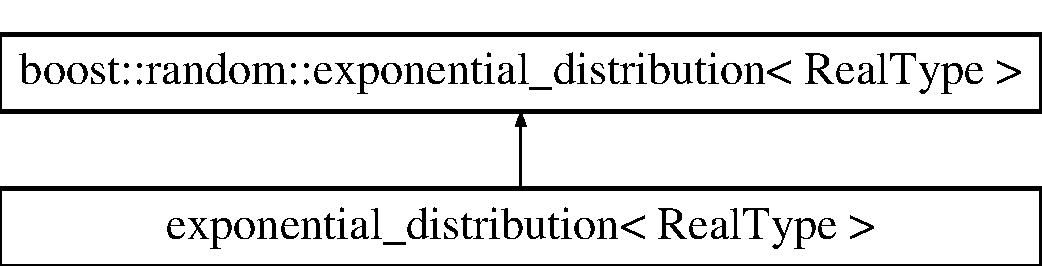
\includegraphics[height=2.000000cm]{structexponential__distribution}
\end{center}
\end{figure}
\subsection*{Public Member Functions}
\begin{DoxyCompactItemize}
\item 
\mbox{\Hypertarget{structexponential__distribution_a7524afbe4ae135246eec0b9900e5fb74}\label{structexponential__distribution_a7524afbe4ae135246eec0b9900e5fb74}} 
\mbox{\hyperlink{structexponential__distribution_a7524afbe4ae135246eec0b9900e5fb74}{exponential\+\_\+distribution}} (Real\+Type \mbox{\hyperlink{structexponential__distribution_a7fcde2f1a6cd1aee2c13300df3663a2f}{lambda}})
\begin{DoxyCompactList}\small\item\em constructor give lambda \end{DoxyCompactList}\item 
\mbox{\Hypertarget{structexponential__distribution_af1d1176f210ca6d4172e916fa71d5266}\label{structexponential__distribution_af1d1176f210ca6d4172e916fa71d5266}} 
Real\+Type \mbox{\hyperlink{structexponential__distribution_af1d1176f210ca6d4172e916fa71d5266}{cdf}} (Real\+Type x, bool lower\+\_\+tail=true) const
\begin{DoxyCompactList}\small\item\em return the cdf or the complement of the cdf \end{DoxyCompactList}\item 
\mbox{\Hypertarget{structexponential__distribution_a1156a5414644c632e98384e09c540a97}\label{structexponential__distribution_a1156a5414644c632e98384e09c540a97}} 
Real\+Type \mbox{\hyperlink{structexponential__distribution_a1156a5414644c632e98384e09c540a97}{pdf}} (Real\+Type x) const
\begin{DoxyCompactList}\small\item\em return the pdf given x \end{DoxyCompactList}\item 
\mbox{\Hypertarget{structexponential__distribution_abaebff9dc27bac0b87dfa5fcc8acdb76}\label{structexponential__distribution_abaebff9dc27bac0b87dfa5fcc8acdb76}} 
Real\+Type \mbox{\hyperlink{structexponential__distribution_abaebff9dc27bac0b87dfa5fcc8acdb76}{quantile}} (Real\+Type p) const
\begin{DoxyCompactList}\small\item\em return the quantile give the probability p \end{DoxyCompactList}\item 
\mbox{\Hypertarget{structexponential__distribution_a7fcde2f1a6cd1aee2c13300df3663a2f}\label{structexponential__distribution_a7fcde2f1a6cd1aee2c13300df3663a2f}} 
Real\+Type \mbox{\hyperlink{structexponential__distribution_a7fcde2f1a6cd1aee2c13300df3663a2f}{lambda}} () const
\begin{DoxyCompactList}\small\item\em return the lambda paramter of the distribution \end{DoxyCompactList}\item 
\mbox{\Hypertarget{structexponential__distribution_a33770c28a6a1d0ab2ffe2bc288cec696}\label{structexponential__distribution_a33770c28a6a1d0ab2ffe2bc288cec696}} 
Real\+Type \mbox{\hyperlink{structexponential__distribution_a33770c28a6a1d0ab2ffe2bc288cec696}{alpha\+\_\+stable}} () const
\begin{DoxyCompactList}\small\item\em return the alpha of the asymptotic stable distribution $\ast$/ \end{DoxyCompactList}\item 
\mbox{\Hypertarget{structexponential__distribution_a3ee0b29c9dd16928c1b53321b361e9fd}\label{structexponential__distribution_a3ee0b29c9dd16928c1b53321b361e9fd}} 
Real\+Type \mbox{\hyperlink{structexponential__distribution_a3ee0b29c9dd16928c1b53321b361e9fd}{mean}} () const
\begin{DoxyCompactList}\small\item\em Return mean of distribution. \end{DoxyCompactList}\item 
\mbox{\Hypertarget{structexponential__distribution_a66bcbe0d4b5ddc9c8b1d1a04ddfbcb6d}\label{structexponential__distribution_a66bcbe0d4b5ddc9c8b1d1a04ddfbcb6d}} 
Real\+Type \mbox{\hyperlink{structexponential__distribution_a66bcbe0d4b5ddc9c8b1d1a04ddfbcb6d}{mad}} () const
\begin{DoxyCompactList}\small\item\em Return mean average deviation of the distribution. \end{DoxyCompactList}\item 
\mbox{\Hypertarget{structexponential__distribution_a8e7d3d592e34ea909a7b0c8bb4807b66}\label{structexponential__distribution_a8e7d3d592e34ea909a7b0c8bb4807b66}} 
Real\+Type \mbox{\hyperlink{structexponential__distribution_a8e7d3d592e34ea909a7b0c8bb4807b66}{mad2}} () const
\begin{DoxyCompactList}\small\item\em Return the mad of the square of the distribution. \end{DoxyCompactList}\item 
\mbox{\Hypertarget{structexponential__distribution_a82795203f013b479354e595a86a4e9c7}\label{structexponential__distribution_a82795203f013b479354e595a86a4e9c7}} 
Real\+Type \mbox{\hyperlink{structexponential__distribution_a82795203f013b479354e595a86a4e9c7}{ci}} (Real\+Type level=Real\+Type(.\+05)) const
\begin{DoxyCompactList}\small\item\em Return the confidence interval of the distribution. \end{DoxyCompactList}\item 
\mbox{\Hypertarget{structexponential__distribution_a2bf78de88b60b9a71773e7eed995f6af}\label{structexponential__distribution_a2bf78de88b60b9a71773e7eed995f6af}} 
complex$<$ Real\+Type $>$ \mbox{\hyperlink{structexponential__distribution_a2bf78de88b60b9a71773e7eed995f6af}{characteristic\+\_\+function}} (Real\+Type omega) const
\begin{DoxyCompactList}\small\item\em return the characteristic function of the distribution given omega \end{DoxyCompactList}\end{DoxyCompactItemize}
\subsection*{Friends}
\begin{DoxyCompactItemize}
\item 
\mbox{\Hypertarget{structexponential__distribution_a0acc132bb35454ce556d35528bdfe8f0}\label{structexponential__distribution_a0acc132bb35454ce556d35528bdfe8f0}} 
{\footnotesize template$<$class charT , class traits $>$ }\\std\+::basic\+\_\+ostream$<$ charT, traits $>$ \& \mbox{\hyperlink{structexponential__distribution_a0acc132bb35454ce556d35528bdfe8f0}{operator$<$$<$}} (std\+::basic\+\_\+ostream$<$ charT, traits $>$ \&os, const \mbox{\hyperlink{structexponential__distribution}{exponential\+\_\+distribution}} \&dist)
\begin{DoxyCompactList}\small\item\em Write distribution to std\+::ostream. \end{DoxyCompactList}\end{DoxyCompactItemize}


\subsection{Detailed Description}
\subsubsection*{template$<$class Real\+Type = double$>$\newline
struct exponential\+\_\+distribution$<$ Real\+Type $>$}

instnaces of sturct \mbox{\hyperlink{structexponential__distribution}{exponential\+\_\+distribution}} generate random variates for exponential distribution 

\begin{DoxyAuthor}{Author}
Created by Joseph Dunn on 1/3/19. 
\end{DoxyAuthor}
\begin{DoxyCopyright}{Copyright}
© 2019 Joseph Dunn. All rights reserved. 
\end{DoxyCopyright}


The documentation for this struct was generated from the following file\+:\begin{DoxyCompactItemize}
\item 
/\+Users/jdunn/\+Documents/\+X\+Code/how\+\_\+much\+\_\+data/convolution\+\_\+test/\mbox{\hyperlink{exponential__distribution_8h}{exponential\+\_\+distribution.\+h}}\end{DoxyCompactItemize}

\hypertarget{structKappaResult}{}\section{Kappa\+Result Struct Reference}
\label{structKappaResult}\index{Kappa\+Result@{Kappa\+Result}}


structure holding the results of a run for a single alpha  


\subsection*{Public Member Functions}
\begin{DoxyCompactItemize}
\item 
\mbox{\hyperlink{structKappaResult_ac0ca82b62ef4f9717ab9e136b251668b}{Kappa\+Result}} (vector$<$ int $>$ \mbox{\hyperlink{structKappaResult_a48d379e6c356ee537839917a67a21c86}{ns}})
\begin{DoxyCompactList}\small\item\em constructor \end{DoxyCompactList}\item 
\mbox{\Hypertarget{structKappaResult_a54228c60b4691f2b1621aa07b1e0437f}\label{structKappaResult_a54228c60b4691f2b1621aa07b1e0437f}} 
void \mbox{\hyperlink{structKappaResult_a54228c60b4691f2b1621aa07b1e0437f}{calc\+\_\+kappa}} ()
\begin{DoxyCompactList}\small\item\em calculate the kappa from the mad and ci variables \end{DoxyCompactList}\item 
void \mbox{\hyperlink{structKappaResult_a73d7fdfa72149f5ec74b22a203f418b9}{initialize}} (double param\+\_\+in, const vector$<$ int $>$ \&ns\+\_\+in)
\begin{DoxyCompactList}\small\item\em initialize the structure \end{DoxyCompactList}\item 
void \mbox{\hyperlink{structKappaResult_ad9a40b7ecb6f56e1e868fd559e07026f}{update\+\_\+dev}} (size\+\_\+t \mbox{\hyperlink{structKappaResult_a5d2264180cefdfefd364065aaf405b72}{m}}, size\+\_\+t \mbox{\hyperlink{structKappaResult_a59f858c0abe9db0eebd82a56665b38df}{m\+\_\+ci}}, const vector$<$ double $>$ \&dev, const vector$<$ double $>$ \&abs\+\_\+dev, const vector$<$ vector$<$ double $>$ $>$ \&x\+\_\+in)
\begin{DoxyCompactList}\small\item\em update the deviations w result from one thread \end{DoxyCompactList}\item 
void \mbox{\hyperlink{structKappaResult_a8dd8b127d34165637298435377489cff}{update\+\_\+conf\+\_\+int}} (double ci\+\_\+level)
\begin{DoxyCompactList}\small\item\em calculate the confidence interval for all trials \end{DoxyCompactList}\end{DoxyCompactItemize}
\subsection*{Public Attributes}
\begin{DoxyCompactItemize}
\item 
\mbox{\Hypertarget{structKappaResult_ac8485e1a2316db98a89d0aecc39e3389}\label{structKappaResult_ac8485e1a2316db98a89d0aecc39e3389}} 
double \mbox{\hyperlink{structKappaResult_ac8485e1a2316db98a89d0aecc39e3389}{param}}
\begin{DoxyCompactList}\small\item\em the parameter for the run \end{DoxyCompactList}\item 
\mbox{\Hypertarget{structKappaResult_a0f841a8ac328e4e7ec24089d31d63efb}\label{structKappaResult_a0f841a8ac328e4e7ec24089d31d63efb}} 
int \mbox{\hyperlink{structKappaResult_a0f841a8ac328e4e7ec24089d31d63efb}{nsize}}
\begin{DoxyCompactList}\small\item\em the size of the vector pased to fft \end{DoxyCompactList}\item 
double \mbox{\hyperlink{structKappaResult_a9fb1e6cd969e50ab18dae7fbf598f949}{mad\+\_\+rel\+\_\+err}}
\begin{DoxyCompactList}\small\item\em the relative error of mad vs theory \end{DoxyCompactList}\item 
vector$<$ int $>$ \mbox{\hyperlink{structKappaResult_a48d379e6c356ee537839917a67a21c86}{ns}}
\begin{DoxyCompactList}\small\item\em the durations saved \end{DoxyCompactList}\item 
\mbox{\Hypertarget{structKappaResult_a43fdcc9f455335e136cb46d2506a14dd}\label{structKappaResult_a43fdcc9f455335e136cb46d2506a14dd}} 
vector$<$ double $>$ \mbox{\hyperlink{structKappaResult_a43fdcc9f455335e136cb46d2506a14dd}{mad}}
\begin{DoxyCompactList}\small\item\em the mean absolute deviation by duration \end{DoxyCompactList}\item 
\mbox{\Hypertarget{structKappaResult_abdbafd17d772e9821b31905d6389c22f}\label{structKappaResult_abdbafd17d772e9821b31905d6389c22f}} 
vector$<$ double $>$ {\bfseries kappa\+\_\+mad}
\item 
double \mbox{\hyperlink{structKappaResult_ae4cbee7f19b10054eec20a22d4cfee02}{ci\+\_\+rel\+\_\+err}}
\begin{DoxyCompactList}\small\item\em the kappa\+\_\+mad by duration \end{DoxyCompactList}\item 
\mbox{\Hypertarget{structKappaResult_ae5f9b611ab3439921432428ad2bdf122}\label{structKappaResult_ae5f9b611ab3439921432428ad2bdf122}} 
vector$<$ double $>$ \mbox{\hyperlink{structKappaResult_ae5f9b611ab3439921432428ad2bdf122}{ci}}
\begin{DoxyCompactList}\small\item\em the conficence interval by duration \end{DoxyCompactList}\item 
\mbox{\Hypertarget{structKappaResult_a04268ef34dd883df399c63bf67b2af26}\label{structKappaResult_a04268ef34dd883df399c63bf67b2af26}} 
vector$<$ double $>$ \mbox{\hyperlink{structKappaResult_a04268ef34dd883df399c63bf67b2af26}{kappa\+\_\+ci}}
\begin{DoxyCompactList}\small\item\em the kappa ci by duration \end{DoxyCompactList}\item 
\mbox{\Hypertarget{structKappaResult_a5d2264180cefdfefd364065aaf405b72}\label{structKappaResult_a5d2264180cefdfefd364065aaf405b72}} 
size\+\_\+t \mbox{\hyperlink{structKappaResult_a5d2264180cefdfefd364065aaf405b72}{m}} = 0
\begin{DoxyCompactList}\small\item\em the number of trials run for mad \end{DoxyCompactList}\item 
\mbox{\Hypertarget{structKappaResult_a59f858c0abe9db0eebd82a56665b38df}\label{structKappaResult_a59f858c0abe9db0eebd82a56665b38df}} 
size\+\_\+t \mbox{\hyperlink{structKappaResult_a59f858c0abe9db0eebd82a56665b38df}{m\+\_\+ci}} = 0
\begin{DoxyCompactList}\small\item\em the number of trials for the conf. interval \end{DoxyCompactList}\item 
\mbox{\Hypertarget{structKappaResult_a133a1322d9761ce51027209c1b344693}\label{structKappaResult_a133a1322d9761ce51027209c1b344693}} 
vector$<$ double $>$ \mbox{\hyperlink{structKappaResult_a133a1322d9761ce51027209c1b344693}{sum\+\_\+dev}}
\begin{DoxyCompactList}\small\item\em sum or raw deviation by duration \end{DoxyCompactList}\item 
\mbox{\Hypertarget{structKappaResult_ab68b3871ee5609c7891ca97336e4e5ce}\label{structKappaResult_ab68b3871ee5609c7891ca97336e4e5ce}} 
vector$<$ double $>$ \mbox{\hyperlink{structKappaResult_ab68b3871ee5609c7891ca97336e4e5ce}{sum\+\_\+abs\+\_\+dev}}
\begin{DoxyCompactList}\small\item\em sum of abs deviations by duration \end{DoxyCompactList}\item 
\mbox{\Hypertarget{structKappaResult_a8680d7947e3911486a4b02403bb4de7c}\label{structKappaResult_a8680d7947e3911486a4b02403bb4de7c}} 
vector$<$ vector$<$ double $>$ $>$ \mbox{\hyperlink{structKappaResult_a8680d7947e3911486a4b02403bb4de7c}{x\+\_\+ci}}
\begin{DoxyCompactList}\small\item\em the results by trial and duration \end{DoxyCompactList}\item 
\mbox{\Hypertarget{structKappaResult_af0a62f7129da61d2fa8cb5107404a6f4}\label{structKappaResult_af0a62f7129da61d2fa8cb5107404a6f4}} 
vector$<$ double $>$ \mbox{\hyperlink{structKappaResult_af0a62f7129da61d2fa8cb5107404a6f4}{conf\+\_\+int}}
\begin{DoxyCompactList}\small\item\em the calculated ci by duration \end{DoxyCompactList}\item 
\mbox{\Hypertarget{structKappaResult_abe1e9dba96dd6eeaef8e34ad73cd5ba8}\label{structKappaResult_abe1e9dba96dd6eeaef8e34ad73cd5ba8}} 
cpu\+\_\+times \mbox{\hyperlink{structKappaResult_abe1e9dba96dd6eeaef8e34ad73cd5ba8}{elapsed\+\_\+time}}
\begin{DoxyCompactList}\small\item\em the elapsed time for the run \end{DoxyCompactList}\end{DoxyCompactItemize}


\subsection{Detailed Description}
structure holding the results of a run for a single alpha 

the struct holding the resutls of a single alpha 

\subsection{Constructor \& Destructor Documentation}
\mbox{\Hypertarget{structKappaResult_ac0ca82b62ef4f9717ab9e136b251668b}\label{structKappaResult_ac0ca82b62ef4f9717ab9e136b251668b}} 
\index{Kappa\+Result@{Kappa\+Result}!Kappa\+Result@{Kappa\+Result}}
\index{Kappa\+Result@{Kappa\+Result}!Kappa\+Result@{Kappa\+Result}}
\subsubsection{\texorpdfstring{Kappa\+Result()}{KappaResult()}}
{\footnotesize\ttfamily Kappa\+Result\+::\+Kappa\+Result (\begin{DoxyParamCaption}\item[{vector$<$ int $>$}]{ns }\end{DoxyParamCaption})\hspace{0.3cm}{\ttfamily [inline]}}



constructor 


\begin{DoxyParams}{Parameters}
{\em ns} & the durations of the output \\
\hline
\end{DoxyParams}


\subsection{Member Function Documentation}
\mbox{\Hypertarget{structKappaResult_a73d7fdfa72149f5ec74b22a203f418b9}\label{structKappaResult_a73d7fdfa72149f5ec74b22a203f418b9}} 
\index{Kappa\+Result@{Kappa\+Result}!initialize@{initialize}}
\index{initialize@{initialize}!Kappa\+Result@{Kappa\+Result}}
\subsubsection{\texorpdfstring{initialize()}{initialize()}}
{\footnotesize\ttfamily void Kappa\+Result\+::initialize (\begin{DoxyParamCaption}\item[{double}]{param\+\_\+in,  }\item[{const vector$<$ int $>$ \&}]{ns\+\_\+in }\end{DoxyParamCaption})\hspace{0.3cm}{\ttfamily [inline]}}



initialize the structure 


\begin{DoxyParams}{Parameters}
{\em param\+\_\+in} & the alpha of the run \\
\hline
{\em ns\+\_\+in} & the durations of the run \\
\hline
\end{DoxyParams}
\mbox{\Hypertarget{structKappaResult_a8dd8b127d34165637298435377489cff}\label{structKappaResult_a8dd8b127d34165637298435377489cff}} 
\index{Kappa\+Result@{Kappa\+Result}!update\+\_\+conf\+\_\+int@{update\+\_\+conf\+\_\+int}}
\index{update\+\_\+conf\+\_\+int@{update\+\_\+conf\+\_\+int}!Kappa\+Result@{Kappa\+Result}}
\subsubsection{\texorpdfstring{update\+\_\+conf\+\_\+int()}{update\_conf\_int()}}
{\footnotesize\ttfamily void Kappa\+Result\+::update\+\_\+conf\+\_\+int (\begin{DoxyParamCaption}\item[{double}]{ci\+\_\+level }\end{DoxyParamCaption})\hspace{0.3cm}{\ttfamily [inline]}}



calculate the confidence interval for all trials 


\begin{DoxyParams}{Parameters}
{\em ci\+\_\+level} & the confidence level to use \\
\hline
\end{DoxyParams}
\mbox{\Hypertarget{structKappaResult_ad9a40b7ecb6f56e1e868fd559e07026f}\label{structKappaResult_ad9a40b7ecb6f56e1e868fd559e07026f}} 
\index{Kappa\+Result@{Kappa\+Result}!update\+\_\+dev@{update\+\_\+dev}}
\index{update\+\_\+dev@{update\+\_\+dev}!Kappa\+Result@{Kappa\+Result}}
\subsubsection{\texorpdfstring{update\+\_\+dev()}{update\_dev()}}
{\footnotesize\ttfamily void Kappa\+Result\+::update\+\_\+dev (\begin{DoxyParamCaption}\item[{size\+\_\+t}]{m,  }\item[{size\+\_\+t}]{m\+\_\+ci,  }\item[{const vector$<$ double $>$ \&}]{dev,  }\item[{const vector$<$ double $>$ \&}]{abs\+\_\+dev,  }\item[{const vector$<$ vector$<$ double $>$ $>$ \&}]{x\+\_\+in }\end{DoxyParamCaption})\hspace{0.3cm}{\ttfamily [inline]}}



update the deviations w result from one thread 


\begin{DoxyParams}{Parameters}
{\em m} & the number of trials for mad \\
\hline
{\em m\+\_\+ci} & the number of trials for ci \\
\hline
{\em dev} & sum of deviation by duration \\
\hline
{\em abs\+\_\+dev} & sum of abs dev by duration \\
\hline
{\em x\+\_\+in} & the variate by trial \\
\hline
\end{DoxyParams}


\subsection{Member Data Documentation}
\mbox{\Hypertarget{structKappaResult_ae4cbee7f19b10054eec20a22d4cfee02}\label{structKappaResult_ae4cbee7f19b10054eec20a22d4cfee02}} 
\index{Kappa\+Result@{Kappa\+Result}!ci\+\_\+rel\+\_\+err@{ci\+\_\+rel\+\_\+err}}
\index{ci\+\_\+rel\+\_\+err@{ci\+\_\+rel\+\_\+err}!Kappa\+Result@{Kappa\+Result}}
\subsubsection{\texorpdfstring{ci\+\_\+rel\+\_\+err}{ci\_rel\_err}}
{\footnotesize\ttfamily double Kappa\+Result\+::ci\+\_\+rel\+\_\+err}



the kappa\+\_\+mad by duration 

the relative error of the ci vs theory

the relative error of conf. int. vs theory \mbox{\Hypertarget{structKappaResult_a9fb1e6cd969e50ab18dae7fbf598f949}\label{structKappaResult_a9fb1e6cd969e50ab18dae7fbf598f949}} 
\index{Kappa\+Result@{Kappa\+Result}!mad\+\_\+rel\+\_\+err@{mad\+\_\+rel\+\_\+err}}
\index{mad\+\_\+rel\+\_\+err@{mad\+\_\+rel\+\_\+err}!Kappa\+Result@{Kappa\+Result}}
\subsubsection{\texorpdfstring{mad\+\_\+rel\+\_\+err}{mad\_rel\_err}}
{\footnotesize\ttfamily double Kappa\+Result\+::mad\+\_\+rel\+\_\+err}



the relative error of mad vs theory 

the relative error of the mad vs theory \mbox{\Hypertarget{structKappaResult_a48d379e6c356ee537839917a67a21c86}\label{structKappaResult_a48d379e6c356ee537839917a67a21c86}} 
\index{Kappa\+Result@{Kappa\+Result}!ns@{ns}}
\index{ns@{ns}!Kappa\+Result@{Kappa\+Result}}
\subsubsection{\texorpdfstring{ns}{ns}}
{\footnotesize\ttfamily vector$<$ int $>$ Kappa\+Result\+::ns}



the durations saved 

the durations calculated 

The documentation for this struct was generated from the following files\+:\begin{DoxyCompactItemize}
\item 
/\+Users/jdunn/\+Documents/\+X\+Code/how\+\_\+much\+\_\+data/convolution\+\_\+test/\mbox{\hyperlink{convolution__test_8cpp}{convolution\+\_\+test.\+cpp}}\item 
/\+Users/jdunn/\+Documents/\+X\+Code/how\+\_\+much\+\_\+data/monte\+\_\+carlo\+\_\+test/\mbox{\hyperlink{monte__carlo__test_8cpp}{monte\+\_\+carlo\+\_\+test.\+cpp}}\end{DoxyCompactItemize}

\hypertarget{structKappaResults}{}\section{Kappa\+Results Struct Reference}
\label{structKappaResults}\index{Kappa\+Results@{Kappa\+Results}}


structure holding the results of all runs  


\subsection*{Public Member Functions}
\begin{DoxyCompactItemize}
\item 
\mbox{\hyperlink{structKappaResults_afec7f4f7947b997b7bb15c308b66c7d4}{Kappa\+Results}} (const vector$<$ int $>$ \&\mbox{\hyperlink{structKappaResults_a4e6a25c186ed54790616474d54a618c3}{ns}}, size\+\_\+t n\+\_\+params, string \mbox{\hyperlink{structKappaResults_a2b42189a3b7690aedacd6d77c05a1c5b}{param\+\_\+label}}, size\+\_\+t \mbox{\hyperlink{structKappaResults_a133dbed775f98f56566b9571ff05746d}{taleb\+\_\+offset}})
\begin{DoxyCompactList}\small\item\em constructor \end{DoxyCompactList}\item 
\mbox{\Hypertarget{structKappaResults_a8b791cd3e214acd7fb951d412f7385bc}\label{structKappaResults_a8b791cd3e214acd7fb951d412f7385bc}} 
\mbox{\hyperlink{structKappaResult}{Kappa\+Result}} \& \mbox{\hyperlink{structKappaResults_a8b791cd3e214acd7fb951d412f7385bc}{at}} (size\+\_\+t i)
\begin{DoxyCompactList}\small\item\em return reference to a particular result \end{DoxyCompactList}\item 
\mbox{\hyperlink{structKappaResults_a914068e2f53f303b501adf0e3b92a468}{Kappa\+Results}} (const vector$<$ int $>$ \&\mbox{\hyperlink{structKappaResults_a4e6a25c186ed54790616474d54a618c3}{ns}}, const vector$<$ double $>$ \&params, const string \mbox{\hyperlink{structKappaResults_a2b42189a3b7690aedacd6d77c05a1c5b}{param\+\_\+label}}, size\+\_\+t \mbox{\hyperlink{structKappaResults_a133dbed775f98f56566b9571ff05746d}{taleb\+\_\+offset}})
\begin{DoxyCompactList}\small\item\em constructor \end{DoxyCompactList}\end{DoxyCompactItemize}
\subsection*{Public Attributes}
\begin{DoxyCompactItemize}
\item 
vector$<$ int $>$ \mbox{\hyperlink{structKappaResults_a4e6a25c186ed54790616474d54a618c3}{ns}}
\begin{DoxyCompactList}\small\item\em the durations saved \end{DoxyCompactList}\item 
string \mbox{\hyperlink{structKappaResults_a2b42189a3b7690aedacd6d77c05a1c5b}{param\+\_\+label}}
\begin{DoxyCompactList}\small\item\em the name of the parameter \end{DoxyCompactList}\item 
\mbox{\Hypertarget{structKappaResults_a2988f98b9b5b70ec1e3ac16e41c57ea2}\label{structKappaResults_a2988f98b9b5b70ec1e3ac16e41c57ea2}} 
vector$<$ \mbox{\hyperlink{structKappaResult}{Kappa\+Result}} $>$ \mbox{\hyperlink{structKappaResults_a2988f98b9b5b70ec1e3ac16e41c57ea2}{kr}}
\begin{DoxyCompactList}\small\item\em the results of the runs by duration \end{DoxyCompactList}\item 
size\+\_\+t \mbox{\hyperlink{structKappaResults_a133dbed775f98f56566b9571ff05746d}{taleb\+\_\+offset}}
\begin{DoxyCompactList}\small\item\em the column offset into Taleb\textquotesingle{}s table \end{DoxyCompactList}\item 
\mbox{\Hypertarget{structKappaResults_a9a2244648ae6ffb1d966bdc414d25240}\label{structKappaResults_a9a2244648ae6ffb1d966bdc414d25240}} 
mutex \mbox{\hyperlink{structKappaResults_a9a2244648ae6ffb1d966bdc414d25240}{kr\+\_\+mutex}}
\begin{DoxyCompactList}\small\item\em a mutex for writing results \end{DoxyCompactList}\end{DoxyCompactItemize}


\subsection{Detailed Description}
structure holding the results of all runs 

sturcture holding the results from all runs 

\subsection{Constructor \& Destructor Documentation}
\mbox{\Hypertarget{structKappaResults_afec7f4f7947b997b7bb15c308b66c7d4}\label{structKappaResults_afec7f4f7947b997b7bb15c308b66c7d4}} 
\index{Kappa\+Results@{Kappa\+Results}!Kappa\+Results@{Kappa\+Results}}
\index{Kappa\+Results@{Kappa\+Results}!Kappa\+Results@{Kappa\+Results}}
\subsubsection{\texorpdfstring{Kappa\+Results()}{KappaResults()}\hspace{0.1cm}{\footnotesize\ttfamily [1/2]}}
{\footnotesize\ttfamily Kappa\+Results\+::\+Kappa\+Results (\begin{DoxyParamCaption}\item[{const vector$<$ int $>$ \&}]{ns,  }\item[{size\+\_\+t}]{n\+\_\+params,  }\item[{string}]{param\+\_\+label,  }\item[{size\+\_\+t}]{taleb\+\_\+offset }\end{DoxyParamCaption})\hspace{0.3cm}{\ttfamily [inline]}}



constructor 


\begin{DoxyParams}{Parameters}
{\em ns} & the durations \\
\hline
{\em n\+\_\+params} & the \# of params \\
\hline
{\em param\+\_\+label} & the param\+\_\+label \\
\hline
{\em taleb\+\_\+offset} & the column offset into Talebs table \\
\hline
\end{DoxyParams}
\mbox{\Hypertarget{structKappaResults_a914068e2f53f303b501adf0e3b92a468}\label{structKappaResults_a914068e2f53f303b501adf0e3b92a468}} 
\index{Kappa\+Results@{Kappa\+Results}!Kappa\+Results@{Kappa\+Results}}
\index{Kappa\+Results@{Kappa\+Results}!Kappa\+Results@{Kappa\+Results}}
\subsubsection{\texorpdfstring{Kappa\+Results()}{KappaResults()}\hspace{0.1cm}{\footnotesize\ttfamily [2/2]}}
{\footnotesize\ttfamily Kappa\+Results\+::\+Kappa\+Results (\begin{DoxyParamCaption}\item[{const vector$<$ int $>$ \&}]{ns,  }\item[{const vector$<$ double $>$ \&}]{params,  }\item[{const string}]{param\+\_\+label,  }\item[{size\+\_\+t}]{taleb\+\_\+offset }\end{DoxyParamCaption})\hspace{0.3cm}{\ttfamily [inline]}}



constructor 


\begin{DoxyParams}{Parameters}
{\em ns} & the durations calculated \\
\hline
{\em params} & the params for each run \\
\hline
{\em param\+\_\+label} & the label for the param \\
\hline
{\em taleb\+\_\+offset} & the column offset into the table of taleg\textquotesingle{}s results. 0 for none \\
\hline
\end{DoxyParams}


\subsection{Member Data Documentation}
\mbox{\Hypertarget{structKappaResults_a4e6a25c186ed54790616474d54a618c3}\label{structKappaResults_a4e6a25c186ed54790616474d54a618c3}} 
\index{Kappa\+Results@{Kappa\+Results}!ns@{ns}}
\index{ns@{ns}!Kappa\+Results@{Kappa\+Results}}
\subsubsection{\texorpdfstring{ns}{ns}}
{\footnotesize\ttfamily vector$<$ int $>$ Kappa\+Results\+::ns}



the durations saved 

the durations calculated \mbox{\Hypertarget{structKappaResults_a2b42189a3b7690aedacd6d77c05a1c5b}\label{structKappaResults_a2b42189a3b7690aedacd6d77c05a1c5b}} 
\index{Kappa\+Results@{Kappa\+Results}!param\+\_\+label@{param\+\_\+label}}
\index{param\+\_\+label@{param\+\_\+label}!Kappa\+Results@{Kappa\+Results}}
\subsubsection{\texorpdfstring{param\+\_\+label}{param\_label}}
{\footnotesize\ttfamily string Kappa\+Results\+::param\+\_\+label}



the name of the parameter 

a vector holding the results of each run the label for the parameter \mbox{\Hypertarget{structKappaResults_a133dbed775f98f56566b9571ff05746d}\label{structKappaResults_a133dbed775f98f56566b9571ff05746d}} 
\index{Kappa\+Results@{Kappa\+Results}!taleb\+\_\+offset@{taleb\+\_\+offset}}
\index{taleb\+\_\+offset@{taleb\+\_\+offset}!Kappa\+Results@{Kappa\+Results}}
\subsubsection{\texorpdfstring{taleb\+\_\+offset}{taleb\_offset}}
{\footnotesize\ttfamily size\+\_\+t Kappa\+Results\+::taleb\+\_\+offset}



the column offset into Taleb\textquotesingle{}s table 

the offset into Taleb\textquotesingle{}s table of results. =0 for none available. 

The documentation for this struct was generated from the following files\+:\begin{DoxyCompactItemize}
\item 
/\+Users/jdunn/\+Documents/\+X\+Code/how\+\_\+much\+\_\+data/convolution\+\_\+test/\mbox{\hyperlink{convolution__test_8cpp}{convolution\+\_\+test.\+cpp}}\item 
/\+Users/jdunn/\+Documents/\+X\+Code/how\+\_\+much\+\_\+data/monte\+\_\+carlo\+\_\+test/\mbox{\hyperlink{monte__carlo__test_8cpp}{monte\+\_\+carlo\+\_\+test.\+cpp}}\end{DoxyCompactItemize}

\hypertarget{structlognormal__distribution}{}\section{lognormal\+\_\+distribution$<$ Real\+Type $>$ Struct Template Reference}
\label{structlognormal__distribution}\index{lognormal\+\_\+distribution$<$ Real\+Type $>$@{lognormal\+\_\+distribution$<$ Real\+Type $>$}}


a class with functions related to the lognormal distribution.  




{\ttfamily \#include $<$lognormal\+\_\+distribution.\+h$>$}

Inheritance diagram for lognormal\+\_\+distribution$<$ Real\+Type $>$\+:\begin{figure}[H]
\begin{center}
\leavevmode
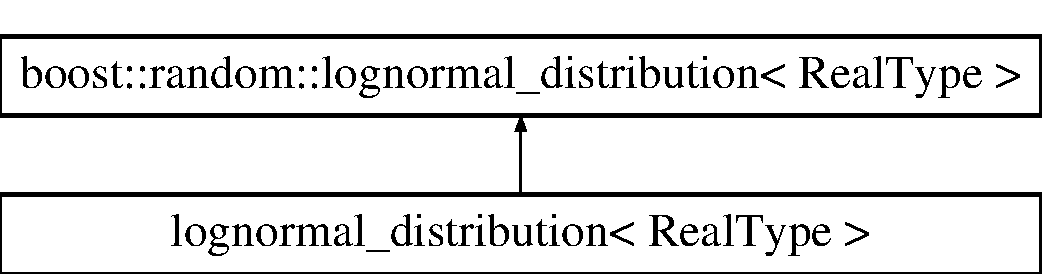
\includegraphics[height=2.000000cm]{structlognormal__distribution}
\end{center}
\end{figure}
\subsection*{Public Member Functions}
\begin{DoxyCompactItemize}
\item 
\mbox{\hyperlink{structlognormal__distribution_a904d491e75ef65ec8bc8373ab40f4dda}{lognormal\+\_\+distribution}} (Real\+Type \mbox{\hyperlink{structlognormal__distribution_aafbea1099645b17baf5a6789e9a17615}{mu}}, Real\+Type \mbox{\hyperlink{structlognormal__distribution_a07a77c8819313d92d38a275ba1c94b55}{sigma}}, Integration\+Controller$<$ Real\+Type $>$ \&cf\+\_\+ctl, int type=1)
\begin{DoxyCompactList}\small\item\em the constructor for the distribution \end{DoxyCompactList}\item 
\mbox{\Hypertarget{structlognormal__distribution_ad8a1fe52287436f6abd5ce60d91bad2c}\label{structlognormal__distribution_ad8a1fe52287436f6abd5ce60d91bad2c}} 
{\footnotesize template$<$typename Engine $>$ }\\Real\+Type \mbox{\hyperlink{structlognormal__distribution_ad8a1fe52287436f6abd5ce60d91bad2c}{operator()}} (Engine \&eng)
\begin{DoxyCompactList}\small\item\em return a random number from the normalized distribution \end{DoxyCompactList}\item 
Real\+Type \mbox{\hyperlink{structlognormal__distribution_a70784d5a2f900ab772c106e6990f176a}{cdf}} (Real\+Type x, bool lower\+\_\+tail=true) const
\begin{DoxyCompactList}\small\item\em return the cumulative distribution function \end{DoxyCompactList}\item 
Real\+Type \mbox{\hyperlink{structlognormal__distribution_a0bf3bc670b041d5015d9a4a88d6220a4}{pdf}} (Real\+Type x) const
\begin{DoxyCompactList}\small\item\em return the probability density function \end{DoxyCompactList}\item 
Real\+Type \mbox{\hyperlink{structlognormal__distribution_ae4e4b312d8225523a204f7e12615b8a2}{quantile}} (Real\+Type p) const
\begin{DoxyCompactList}\small\item\em return the quantile corresponding to a given propability \end{DoxyCompactList}\item 
\mbox{\Hypertarget{structlognormal__distribution_aafbea1099645b17baf5a6789e9a17615}\label{structlognormal__distribution_aafbea1099645b17baf5a6789e9a17615}} 
Real\+Type \mbox{\hyperlink{structlognormal__distribution_aafbea1099645b17baf5a6789e9a17615}{mu}} () const
\begin{DoxyCompactList}\small\item\em return the mu parameter of the distribution \end{DoxyCompactList}\item 
\mbox{\Hypertarget{structlognormal__distribution_a07a77c8819313d92d38a275ba1c94b55}\label{structlognormal__distribution_a07a77c8819313d92d38a275ba1c94b55}} 
Real\+Type \mbox{\hyperlink{structlognormal__distribution_a07a77c8819313d92d38a275ba1c94b55}{sigma}} () const
\begin{DoxyCompactList}\small\item\em return sigma parameter of the distribution \end{DoxyCompactList}\item 
\mbox{\Hypertarget{structlognormal__distribution_a9ca440314fb852a6dbad4ebd4ddb7573}\label{structlognormal__distribution_a9ca440314fb852a6dbad4ebd4ddb7573}} 
Real\+Type \mbox{\hyperlink{structlognormal__distribution_a9ca440314fb852a6dbad4ebd4ddb7573}{alpha\+\_\+stable}} () const
\begin{DoxyCompactList}\small\item\em return the alpha parameter of the asymptotically equivalent stable distribution \end{DoxyCompactList}\item 
Real\+Type \mbox{\hyperlink{structlognormal__distribution_afedf3fef881e7b36d429b50f34ef1573}{min}} () const
\begin{DoxyCompactList}\small\item\em Returns the smallest value that the distribution can produce. \end{DoxyCompactList}\item 
Real\+Type \mbox{\hyperlink{structlognormal__distribution_a2de6f05fe434834c076a67fafc311357}{max}} () const
\begin{DoxyCompactList}\small\item\em Returns the largest value that the distribution can produce. \end{DoxyCompactList}\item 
\mbox{\Hypertarget{structlognormal__distribution_a59152655fdac026bc8a8eb8abadc247f}\label{structlognormal__distribution_a59152655fdac026bc8a8eb8abadc247f}} 
Real\+Type \mbox{\hyperlink{structlognormal__distribution_a59152655fdac026bc8a8eb8abadc247f}{mean}} () const
\begin{DoxyCompactList}\small\item\em Return mean of distribution. \end{DoxyCompactList}\item 
\mbox{\Hypertarget{structlognormal__distribution_ac7b2143d799524dd1c4e2661225ff6c7}\label{structlognormal__distribution_ac7b2143d799524dd1c4e2661225ff6c7}} 
Real\+Type \mbox{\hyperlink{structlognormal__distribution_ac7b2143d799524dd1c4e2661225ff6c7}{mad}} () const
\begin{DoxyCompactList}\small\item\em Return mean absolute deviation of the distribution. \end{DoxyCompactList}\item 
Real\+Type \mbox{\hyperlink{structlognormal__distribution_a41c93e0aac16e184161abc486a61319a}{mad2}} () const
\begin{DoxyCompactList}\small\item\em Return the mad of the square of the distribution. \end{DoxyCompactList}\item 
\mbox{\Hypertarget{structlognormal__distribution_ab2ecb3bc59203c7ea4acfe8a1d3ab332}\label{structlognormal__distribution_ab2ecb3bc59203c7ea4acfe8a1d3ab332}} 
Real\+Type \mbox{\hyperlink{structlognormal__distribution_ab2ecb3bc59203c7ea4acfe8a1d3ab332}{ci}} (Real\+Type level=Real\+Type(.\+05)) const
\begin{DoxyCompactList}\small\item\em Return the confidence interval of the distribution. \end{DoxyCompactList}\item 
complex$<$ Real\+Type $>$ \mbox{\hyperlink{structlognormal__distribution_a46b1bc0ea6c8a46bc341165be2ca47fe}{cf\+\_\+series}} (complex$<$ Real\+Type $>$ omega, Real\+Type $\ast$\+\_\+error=nullptr, Real\+Type $\ast$\+\_\+l1\+\_\+norm=nullptr, int $\ast$\+\_\+neval=nullptr)
\begin{DoxyCompactList}\small\item\em cf via asymptotic series for small omega \end{DoxyCompactList}\item 
complex$<$ Real\+Type $>$ \mbox{\hyperlink{structlognormal__distribution_a0a0adae1494c1614dc15ff7f4c5a9a02}{cfprime\+\_\+series}} (complex$<$ Real\+Type $>$ omega, Real\+Type $\ast$\+\_\+error=nullptr, Real\+Type $\ast$\+\_\+l1\+\_\+norm=nullptr, int $\ast$\+\_\+neval=nullptr)
\begin{DoxyCompactList}\small\item\em derivative of cf via asymptotic series for small omega \end{DoxyCompactList}\item 
complex$<$ Real\+Type $>$ \mbox{\hyperlink{structlognormal__distribution_a8764320a4993baf3b2c37e84e85f5930}{cf\+\_\+lambert\+\_\+w}} (complex$<$ Real\+Type $>$ omega, Real\+Type $\ast$\+\_\+error=nullptr, Real\+Type $\ast$\+\_\+l1\+\_\+norm=nullptr, int $\ast$\+\_\+neval=nullptr)
\begin{DoxyCompactList}\small\item\em Much faster than either integral but has problems when sigma $>$ 1. \end{DoxyCompactList}\item 
complex$<$ Real\+Type $>$ \mbox{\hyperlink{structlognormal__distribution_a21c4d9822769e84f959dca1bb741517f}{cfprime\+\_\+lambert\+\_\+w}} (complex$<$ Real\+Type $>$ omega, Real\+Type $\ast$\+\_\+error=nullptr, Real\+Type $\ast$\+\_\+l1\+\_\+norm=nullptr, int $\ast$\+\_\+neval=nullptr)
\begin{DoxyCompactList}\small\item\em return the approximate derivative of char. \end{DoxyCompactList}\item 
complex$<$ Real\+Type $>$ \mbox{\hyperlink{structlognormal__distribution_adb0238c0eed40f4e32f4ad35a107caee}{cf\+\_\+fourier}} (complex$<$ Real\+Type $>$ omega, Real\+Type $\ast$\+\_\+error=nullptr, Real\+Type $\ast$\+\_\+l1\+\_\+norm=nullptr, int $\ast$\+\_\+neval=nullptr)
\begin{DoxyCompactList}\small\item\em Return the characteristic function along a designer countour. \end{DoxyCompactList}\item 
complex$<$ Real\+Type $>$ \mbox{\hyperlink{structlognormal__distribution_af833fd54866c0c6a651b96c198294a11}{cfprime\+\_\+fourier}} (complex$<$ Real\+Type $>$ omega, Real\+Type $\ast$\+\_\+error=nullptr, Real\+Type $\ast$\+\_\+l1\+\_\+norm=nullptr, int $\ast$\+\_\+neval=nullptr)
\begin{DoxyCompactList}\small\item\em Return the derivative of the char. fun. wrt omega using designer contour. \end{DoxyCompactList}\item 
complex$<$ Real\+Type $>$ \mbox{\hyperlink{structlognormal__distribution_ab0a44ee2aad7c6f19cb4e3c930b993bd}{cf\+\_\+fourier\+\_\+lnx}} (complex$<$ Real\+Type $>$ omega, Real\+Type $\ast$\+\_\+error=nullptr, Real\+Type $\ast$\+\_\+l1\+\_\+norm=nullptr, int $\ast$\+\_\+neval=nullptr)
\begin{DoxyCompactList}\small\item\em Return the characteristic function via Fourier integral in ln(x) domain. \end{DoxyCompactList}\item 
complex$<$ Real\+Type $>$ \mbox{\hyperlink{structlognormal__distribution_adcd4b3eee23e964a17e6cbc701142d3f}{cfprime\+\_\+fourier\+\_\+lnx}} (complex$<$ Real\+Type $>$ omega, Real\+Type $\ast$\+\_\+error=nullptr, Real\+Type $\ast$\+\_\+l1\+\_\+norm=nullptr, int $\ast$\+\_\+neval=nullptr)
\begin{DoxyCompactList}\small\item\em Return the derivative of char. function via Fourier integral in ln(x) domain. \end{DoxyCompactList}\item 
complex$<$ Real\+Type $>$ \mbox{\hyperlink{structlognormal__distribution_a969271c41bfb153c8983ef0dc1813a6b}{cf\+\_\+fourier\+\_\+mixed}} (complex$<$ Real\+Type $>$ omega, Real\+Type $\ast$\+\_\+error=nullptr, Real\+Type $\ast$\+\_\+l1\+\_\+norm=nullptr, int $\ast$\+\_\+neval=nullptr)
\begin{DoxyCompactList}\small\item\em Return the characteristic function via Fourier integral in ln(x) domain. \end{DoxyCompactList}\item 
complex$<$ Real\+Type $>$ \mbox{\hyperlink{structlognormal__distribution_a3760cd4c0612e34e49edd896f10a03ae}{cfprime\+\_\+fourier\+\_\+mixed}} (complex$<$ Real\+Type $>$ omega, Real\+Type $\ast$\+\_\+error=nullptr, Real\+Type $\ast$\+\_\+l1\+\_\+norm=nullptr, int $\ast$\+\_\+neval=nullptr)
\begin{DoxyCompactList}\small\item\em The derivative of the char. fun. using mixed Lambert and shifted contour. \end{DoxyCompactList}\item 
complex$<$ Real\+Type $>$ \mbox{\hyperlink{structlognormal__distribution_a2b8eebf8ea44cd27b6fc3dd265cbcfe8}{characteristic\+\_\+function}} (complex$<$ Real\+Type $>$ omega, Real\+Type $\ast$\+\_\+error=nullptr, Real\+Type $\ast$\+\_\+l1\+\_\+norm=nullptr, int $\ast$\+\_\+neval=nullptr)
\begin{DoxyCompactList}\small\item\em return the approximate characteristic function \end{DoxyCompactList}\item 
complex$<$ Real\+Type $>$ \mbox{\hyperlink{structlognormal__distribution_ac46cfb90dfcffb18d7cd11423317bb5c}{characteristic\+\_\+function\+\_\+prime}} (complex$<$ Real\+Type $>$ omega, Real\+Type $\ast$\+\_\+error=nullptr, Real\+Type $\ast$\+\_\+l1\+\_\+norm=nullptr, int $\ast$\+\_\+neval=nullptr)
\begin{DoxyCompactList}\small\item\em return the derivative of the characteristic function \end{DoxyCompactList}\end{DoxyCompactItemize}
\subsection*{Static Public Member Functions}
\begin{DoxyCompactItemize}
\item 
\mbox{\Hypertarget{structlognormal__distribution_abaff10903e63f6b4a45a79dcf36e3ce3}\label{structlognormal__distribution_abaff10903e63f6b4a45a79dcf36e3ce3}} 
static void \mbox{\hyperlink{structlognormal__distribution_abaff10903e63f6b4a45a79dcf36e3ce3}{print\+\_\+fourier\+\_\+integrand}} (ostream \&os, int n, complex$<$ Real\+Type $>$ omega, Real\+Type \mbox{\hyperlink{structlognormal__distribution_a07a77c8819313d92d38a275ba1c94b55}{sigma}})
\begin{DoxyCompactList}\small\item\em print integrand of C\+F\+Integrand \end{DoxyCompactList}\end{DoxyCompactItemize}
\subsection*{Friends}
\begin{DoxyCompactItemize}
\item 
\mbox{\Hypertarget{structlognormal__distribution_a67d222a97b33b757988e03549c9449bb}\label{structlognormal__distribution_a67d222a97b33b757988e03549c9449bb}} 
{\footnotesize template$<$class charT , class traits $>$ }\\std\+::basic\+\_\+ostream$<$ charT, traits $>$ \& \mbox{\hyperlink{structlognormal__distribution_a67d222a97b33b757988e03549c9449bb}{operator$<$$<$}} (std\+::basic\+\_\+ostream$<$ charT, traits $>$ \&os, const \mbox{\hyperlink{structlognormal__distribution}{lognormal\+\_\+distribution}} \&dist)
\begin{DoxyCompactList}\small\item\em Write distribution to std\+::ostream. \end{DoxyCompactList}\end{DoxyCompactItemize}


\subsection{Detailed Description}
\subsubsection*{template$<$class Real\+Type = double$>$\newline
struct lognormal\+\_\+distribution$<$ Real\+Type $>$}

a class with functions related to the lognormal distribution. 

Describes a random variable distributed as exp(sigma X + mu) adjusted to zero mean where X is normally distributed. 

\subsection{Constructor \& Destructor Documentation}
\mbox{\Hypertarget{structlognormal__distribution_a904d491e75ef65ec8bc8373ab40f4dda}\label{structlognormal__distribution_a904d491e75ef65ec8bc8373ab40f4dda}} 
\index{lognormal\+\_\+distribution@{lognormal\+\_\+distribution}!lognormal\+\_\+distribution@{lognormal\+\_\+distribution}}
\index{lognormal\+\_\+distribution@{lognormal\+\_\+distribution}!lognormal\+\_\+distribution@{lognormal\+\_\+distribution}}
\subsubsection{\texorpdfstring{lognormal\+\_\+distribution()}{lognormal\_distribution()}}
{\footnotesize\ttfamily template$<$class Real\+Type  = double$>$ \\
\mbox{\hyperlink{structlognormal__distribution}{lognormal\+\_\+distribution}}$<$ Real\+Type $>$\+::\mbox{\hyperlink{structlognormal__distribution}{lognormal\+\_\+distribution}} (\begin{DoxyParamCaption}\item[{Real\+Type}]{mu,  }\item[{Real\+Type}]{sigma,  }\item[{Integration\+Controller$<$ Real\+Type $>$ \&}]{cf\+\_\+ctl,  }\item[{int}]{type = {\ttfamily 1} }\end{DoxyParamCaption})\hspace{0.3cm}{\ttfamily [inline]}}



the constructor for the distribution 


\begin{DoxyParams}[1]{Parameters}
\mbox{\tt in}  & {\em mu} & the mu parameter \\
\hline
\mbox{\tt in}  & {\em sigma} & the sigma parameter \\
\hline
 & {\em cf\+\_\+ctl} & \mbox{[}in\} reference controller \\
\hline
\mbox{\tt in}  & {\em type} & type of cf calculaiton 1 ln(x), 2 bespoke, 3 w, 4 mixed \\
\hline
\end{DoxyParams}


\subsection{Member Function Documentation}
\mbox{\Hypertarget{structlognormal__distribution_a70784d5a2f900ab772c106e6990f176a}\label{structlognormal__distribution_a70784d5a2f900ab772c106e6990f176a}} 
\index{lognormal\+\_\+distribution@{lognormal\+\_\+distribution}!cdf@{cdf}}
\index{cdf@{cdf}!lognormal\+\_\+distribution@{lognormal\+\_\+distribution}}
\subsubsection{\texorpdfstring{cdf()}{cdf()}}
{\footnotesize\ttfamily template$<$class Real\+Type  = double$>$ \\
Real\+Type \mbox{\hyperlink{structlognormal__distribution}{lognormal\+\_\+distribution}}$<$ Real\+Type $>$\+::cdf (\begin{DoxyParamCaption}\item[{Real\+Type}]{x,  }\item[{bool}]{lower\+\_\+tail = {\ttfamily true} }\end{DoxyParamCaption}) const\hspace{0.3cm}{\ttfamily [inline]}}



return the cumulative distribution function 


\begin{DoxyParams}[1]{Parameters}
\mbox{\tt in}  & {\em x} & the quantile variable \\
\hline
\mbox{\tt in}  & {\em lower\+\_\+tail} & flag indicating which tail to use \\
\hline
\end{DoxyParams}
\mbox{\Hypertarget{structlognormal__distribution_adb0238c0eed40f4e32f4ad35a107caee}\label{structlognormal__distribution_adb0238c0eed40f4e32f4ad35a107caee}} 
\index{lognormal\+\_\+distribution@{lognormal\+\_\+distribution}!cf\+\_\+fourier@{cf\+\_\+fourier}}
\index{cf\+\_\+fourier@{cf\+\_\+fourier}!lognormal\+\_\+distribution@{lognormal\+\_\+distribution}}
\subsubsection{\texorpdfstring{cf\+\_\+fourier()}{cf\_fourier()}}
{\footnotesize\ttfamily template$<$class Real\+Type  = double$>$ \\
complex$<$Real\+Type$>$ \mbox{\hyperlink{structlognormal__distribution}{lognormal\+\_\+distribution}}$<$ Real\+Type $>$\+::cf\+\_\+fourier (\begin{DoxyParamCaption}\item[{complex$<$ Real\+Type $>$}]{omega,  }\item[{Real\+Type $\ast$}]{\+\_\+error = {\ttfamily nullptr},  }\item[{Real\+Type $\ast$}]{\+\_\+l1\+\_\+norm = {\ttfamily nullptr},  }\item[{int $\ast$}]{\+\_\+neval = {\ttfamily nullptr} }\end{DoxyParamCaption})\hspace{0.3cm}{\ttfamily [inline]}}



Return the characteristic function along a designer countour. 


\begin{DoxyParams}[1]{Parameters}
 & {\em omega} & the angular frequency \\
\hline
\mbox{\tt out}  & {\em \+\_\+error} & the integration error \\
\hline
\mbox{\tt out}  & {\em \+\_\+l1\+\_\+norm} & the l1 norm \\
\hline
\mbox{\tt out}  & {\em \+\_\+neval} & the \# of evaluations \\
\hline
\end{DoxyParams}
\mbox{\Hypertarget{structlognormal__distribution_ab0a44ee2aad7c6f19cb4e3c930b993bd}\label{structlognormal__distribution_ab0a44ee2aad7c6f19cb4e3c930b993bd}} 
\index{lognormal\+\_\+distribution@{lognormal\+\_\+distribution}!cf\+\_\+fourier\+\_\+lnx@{cf\+\_\+fourier\+\_\+lnx}}
\index{cf\+\_\+fourier\+\_\+lnx@{cf\+\_\+fourier\+\_\+lnx}!lognormal\+\_\+distribution@{lognormal\+\_\+distribution}}
\subsubsection{\texorpdfstring{cf\+\_\+fourier\+\_\+lnx()}{cf\_fourier\_lnx()}}
{\footnotesize\ttfamily template$<$class Real\+Type  = double$>$ \\
complex$<$Real\+Type$>$ \mbox{\hyperlink{structlognormal__distribution}{lognormal\+\_\+distribution}}$<$ Real\+Type $>$\+::cf\+\_\+fourier\+\_\+lnx (\begin{DoxyParamCaption}\item[{complex$<$ Real\+Type $>$}]{omega,  }\item[{Real\+Type $\ast$}]{\+\_\+error = {\ttfamily nullptr},  }\item[{Real\+Type $\ast$}]{\+\_\+l1\+\_\+norm = {\ttfamily nullptr},  }\item[{int $\ast$}]{\+\_\+neval = {\ttfamily nullptr} }\end{DoxyParamCaption})\hspace{0.3cm}{\ttfamily [inline]}}



Return the characteristic function via Fourier integral in ln(x) domain. 


\begin{DoxyParams}[1]{Parameters}
 & {\em omega} & the angular frequency \\
\hline
\mbox{\tt out}  & {\em \+\_\+error} & the integration error \\
\hline
\mbox{\tt out}  & {\em \+\_\+l1\+\_\+norm} & the \\
\hline
\mbox{\tt out}  & {\em \+\_\+neval} & the \# of evaluations \\
\hline
\end{DoxyParams}
\mbox{\Hypertarget{structlognormal__distribution_a969271c41bfb153c8983ef0dc1813a6b}\label{structlognormal__distribution_a969271c41bfb153c8983ef0dc1813a6b}} 
\index{lognormal\+\_\+distribution@{lognormal\+\_\+distribution}!cf\+\_\+fourier\+\_\+mixed@{cf\+\_\+fourier\+\_\+mixed}}
\index{cf\+\_\+fourier\+\_\+mixed@{cf\+\_\+fourier\+\_\+mixed}!lognormal\+\_\+distribution@{lognormal\+\_\+distribution}}
\subsubsection{\texorpdfstring{cf\+\_\+fourier\+\_\+mixed()}{cf\_fourier\_mixed()}}
{\footnotesize\ttfamily template$<$class Real\+Type  = double$>$ \\
complex$<$Real\+Type$>$ \mbox{\hyperlink{structlognormal__distribution}{lognormal\+\_\+distribution}}$<$ Real\+Type $>$\+::cf\+\_\+fourier\+\_\+mixed (\begin{DoxyParamCaption}\item[{complex$<$ Real\+Type $>$}]{omega,  }\item[{Real\+Type $\ast$}]{\+\_\+error = {\ttfamily nullptr},  }\item[{Real\+Type $\ast$}]{\+\_\+l1\+\_\+norm = {\ttfamily nullptr},  }\item[{int $\ast$}]{\+\_\+neval = {\ttfamily nullptr} }\end{DoxyParamCaption})\hspace{0.3cm}{\ttfamily [inline]}}



Return the characteristic function via Fourier integral in ln(x) domain. 


\begin{DoxyParams}[1]{Parameters}
 & {\em omega} & the angular frequency \\
\hline
\mbox{\tt out}  & {\em \+\_\+error} & the integration error \\
\hline
\mbox{\tt out}  & {\em \+\_\+l1\+\_\+norm} & the \\
\hline
\mbox{\tt out}  & {\em \+\_\+neval} & the \# of evaluations \\
\hline
\end{DoxyParams}
\mbox{\Hypertarget{structlognormal__distribution_a8764320a4993baf3b2c37e84e85f5930}\label{structlognormal__distribution_a8764320a4993baf3b2c37e84e85f5930}} 
\index{lognormal\+\_\+distribution@{lognormal\+\_\+distribution}!cf\+\_\+lambert\+\_\+w@{cf\+\_\+lambert\+\_\+w}}
\index{cf\+\_\+lambert\+\_\+w@{cf\+\_\+lambert\+\_\+w}!lognormal\+\_\+distribution@{lognormal\+\_\+distribution}}
\subsubsection{\texorpdfstring{cf\+\_\+lambert\+\_\+w()}{cf\_lambert\_w()}}
{\footnotesize\ttfamily template$<$class Real\+Type  = double$>$ \\
complex$<$Real\+Type$>$ \mbox{\hyperlink{structlognormal__distribution}{lognormal\+\_\+distribution}}$<$ Real\+Type $>$\+::cf\+\_\+lambert\+\_\+w (\begin{DoxyParamCaption}\item[{complex$<$ Real\+Type $>$}]{omega,  }\item[{Real\+Type $\ast$}]{\+\_\+error = {\ttfamily nullptr},  }\item[{Real\+Type $\ast$}]{\+\_\+l1\+\_\+norm = {\ttfamily nullptr},  }\item[{int $\ast$}]{\+\_\+neval = {\ttfamily nullptr} }\end{DoxyParamCaption})\hspace{0.3cm}{\ttfamily [inline]}}



Much faster than either integral but has problems when sigma $>$ 1. 


\begin{DoxyParams}[1]{Parameters}
 & {\em omega} & the angular frequency \\
\hline
\mbox{\tt out}  & {\em \+\_\+error} & the integration error \\
\hline
\mbox{\tt out}  & {\em \+\_\+l1\+\_\+norm} & the \\
\hline
\mbox{\tt out}  & {\em \+\_\+neval} & the \# of evaluations \\
\hline
\end{DoxyParams}
\mbox{\Hypertarget{structlognormal__distribution_a46b1bc0ea6c8a46bc341165be2ca47fe}\label{structlognormal__distribution_a46b1bc0ea6c8a46bc341165be2ca47fe}} 
\index{lognormal\+\_\+distribution@{lognormal\+\_\+distribution}!cf\+\_\+series@{cf\+\_\+series}}
\index{cf\+\_\+series@{cf\+\_\+series}!lognormal\+\_\+distribution@{lognormal\+\_\+distribution}}
\subsubsection{\texorpdfstring{cf\+\_\+series()}{cf\_series()}}
{\footnotesize\ttfamily template$<$class Real\+Type  = double$>$ \\
complex$<$Real\+Type$>$ \mbox{\hyperlink{structlognormal__distribution}{lognormal\+\_\+distribution}}$<$ Real\+Type $>$\+::cf\+\_\+series (\begin{DoxyParamCaption}\item[{complex$<$ Real\+Type $>$}]{omega,  }\item[{Real\+Type $\ast$}]{\+\_\+error = {\ttfamily nullptr},  }\item[{Real\+Type $\ast$}]{\+\_\+l1\+\_\+norm = {\ttfamily nullptr},  }\item[{int $\ast$}]{\+\_\+neval = {\ttfamily nullptr} }\end{DoxyParamCaption})\hspace{0.3cm}{\ttfamily [inline]}}



cf via asymptotic series for small omega 


\begin{DoxyParams}[1]{Parameters}
 & {\em omega} & the angular frequency \\
\hline
\mbox{\tt out}  & {\em \+\_\+error} & the integration error \\
\hline
\mbox{\tt out}  & {\em \+\_\+l1\+\_\+norm} & the l1 norm \\
\hline
\mbox{\tt out}  & {\em \+\_\+neval} & the \# of evaluations \\
\hline
\end{DoxyParams}
\mbox{\Hypertarget{structlognormal__distribution_af833fd54866c0c6a651b96c198294a11}\label{structlognormal__distribution_af833fd54866c0c6a651b96c198294a11}} 
\index{lognormal\+\_\+distribution@{lognormal\+\_\+distribution}!cfprime\+\_\+fourier@{cfprime\+\_\+fourier}}
\index{cfprime\+\_\+fourier@{cfprime\+\_\+fourier}!lognormal\+\_\+distribution@{lognormal\+\_\+distribution}}
\subsubsection{\texorpdfstring{cfprime\+\_\+fourier()}{cfprime\_fourier()}}
{\footnotesize\ttfamily template$<$class Real\+Type  = double$>$ \\
complex$<$Real\+Type$>$ \mbox{\hyperlink{structlognormal__distribution}{lognormal\+\_\+distribution}}$<$ Real\+Type $>$\+::cfprime\+\_\+fourier (\begin{DoxyParamCaption}\item[{complex$<$ Real\+Type $>$}]{omega,  }\item[{Real\+Type $\ast$}]{\+\_\+error = {\ttfamily nullptr},  }\item[{Real\+Type $\ast$}]{\+\_\+l1\+\_\+norm = {\ttfamily nullptr},  }\item[{int $\ast$}]{\+\_\+neval = {\ttfamily nullptr} }\end{DoxyParamCaption})\hspace{0.3cm}{\ttfamily [inline]}}



Return the derivative of the char. fun. wrt omega using designer contour. 


\begin{DoxyParams}[1]{Parameters}
 & {\em omega} & the angular frequency \\
\hline
\mbox{\tt out}  & {\em \+\_\+error} & the integration error \\
\hline
\mbox{\tt out}  & {\em \+\_\+l1\+\_\+norm} & the \\
\hline
 & {\em \+\_\+neval} & the number of evaluations \\
\hline
\end{DoxyParams}
\mbox{\Hypertarget{structlognormal__distribution_adcd4b3eee23e964a17e6cbc701142d3f}\label{structlognormal__distribution_adcd4b3eee23e964a17e6cbc701142d3f}} 
\index{lognormal\+\_\+distribution@{lognormal\+\_\+distribution}!cfprime\+\_\+fourier\+\_\+lnx@{cfprime\+\_\+fourier\+\_\+lnx}}
\index{cfprime\+\_\+fourier\+\_\+lnx@{cfprime\+\_\+fourier\+\_\+lnx}!lognormal\+\_\+distribution@{lognormal\+\_\+distribution}}
\subsubsection{\texorpdfstring{cfprime\+\_\+fourier\+\_\+lnx()}{cfprime\_fourier\_lnx()}}
{\footnotesize\ttfamily template$<$class Real\+Type  = double$>$ \\
complex$<$Real\+Type$>$ \mbox{\hyperlink{structlognormal__distribution}{lognormal\+\_\+distribution}}$<$ Real\+Type $>$\+::cfprime\+\_\+fourier\+\_\+lnx (\begin{DoxyParamCaption}\item[{complex$<$ Real\+Type $>$}]{omega,  }\item[{Real\+Type $\ast$}]{\+\_\+error = {\ttfamily nullptr},  }\item[{Real\+Type $\ast$}]{\+\_\+l1\+\_\+norm = {\ttfamily nullptr},  }\item[{int $\ast$}]{\+\_\+neval = {\ttfamily nullptr} }\end{DoxyParamCaption})\hspace{0.3cm}{\ttfamily [inline]}}



Return the derivative of char. function via Fourier integral in ln(x) domain. 


\begin{DoxyParams}[1]{Parameters}
 & {\em omega} & the angular frequency \\
\hline
\mbox{\tt out}  & {\em \+\_\+error} & the integration error \\
\hline
\mbox{\tt out}  & {\em \+\_\+l1\+\_\+norm} & the \\
\hline
\mbox{\tt out}  & {\em \+\_\+neval} & the \# of evaluations \\
\hline
\end{DoxyParams}
\mbox{\Hypertarget{structlognormal__distribution_a3760cd4c0612e34e49edd896f10a03ae}\label{structlognormal__distribution_a3760cd4c0612e34e49edd896f10a03ae}} 
\index{lognormal\+\_\+distribution@{lognormal\+\_\+distribution}!cfprime\+\_\+fourier\+\_\+mixed@{cfprime\+\_\+fourier\+\_\+mixed}}
\index{cfprime\+\_\+fourier\+\_\+mixed@{cfprime\+\_\+fourier\+\_\+mixed}!lognormal\+\_\+distribution@{lognormal\+\_\+distribution}}
\subsubsection{\texorpdfstring{cfprime\+\_\+fourier\+\_\+mixed()}{cfprime\_fourier\_mixed()}}
{\footnotesize\ttfamily template$<$class Real\+Type  = double$>$ \\
complex$<$Real\+Type$>$ \mbox{\hyperlink{structlognormal__distribution}{lognormal\+\_\+distribution}}$<$ Real\+Type $>$\+::cfprime\+\_\+fourier\+\_\+mixed (\begin{DoxyParamCaption}\item[{complex$<$ Real\+Type $>$}]{omega,  }\item[{Real\+Type $\ast$}]{\+\_\+error = {\ttfamily nullptr},  }\item[{Real\+Type $\ast$}]{\+\_\+l1\+\_\+norm = {\ttfamily nullptr},  }\item[{int $\ast$}]{\+\_\+neval = {\ttfamily nullptr} }\end{DoxyParamCaption})\hspace{0.3cm}{\ttfamily [inline]}}



The derivative of the char. fun. using mixed Lambert and shifted contour. 


\begin{DoxyParams}[1]{Parameters}
 & {\em omega} & the angular frequency \\
\hline
\mbox{\tt out}  & {\em \+\_\+error} & the integration error \\
\hline
\mbox{\tt out}  & {\em \+\_\+l1\+\_\+norm} & the \\
\hline
\mbox{\tt out}  & {\em \+\_\+neval} & the \# of evaluations \\
\hline
\end{DoxyParams}
\mbox{\Hypertarget{structlognormal__distribution_a21c4d9822769e84f959dca1bb741517f}\label{structlognormal__distribution_a21c4d9822769e84f959dca1bb741517f}} 
\index{lognormal\+\_\+distribution@{lognormal\+\_\+distribution}!cfprime\+\_\+lambert\+\_\+w@{cfprime\+\_\+lambert\+\_\+w}}
\index{cfprime\+\_\+lambert\+\_\+w@{cfprime\+\_\+lambert\+\_\+w}!lognormal\+\_\+distribution@{lognormal\+\_\+distribution}}
\subsubsection{\texorpdfstring{cfprime\+\_\+lambert\+\_\+w()}{cfprime\_lambert\_w()}}
{\footnotesize\ttfamily template$<$class Real\+Type  = double$>$ \\
complex$<$Real\+Type$>$ \mbox{\hyperlink{structlognormal__distribution}{lognormal\+\_\+distribution}}$<$ Real\+Type $>$\+::cfprime\+\_\+lambert\+\_\+w (\begin{DoxyParamCaption}\item[{complex$<$ Real\+Type $>$}]{omega,  }\item[{Real\+Type $\ast$}]{\+\_\+error = {\ttfamily nullptr},  }\item[{Real\+Type $\ast$}]{\+\_\+l1\+\_\+norm = {\ttfamily nullptr},  }\item[{int $\ast$}]{\+\_\+neval = {\ttfamily nullptr} }\end{DoxyParamCaption})\hspace{0.3cm}{\ttfamily [inline]}}



return the approximate derivative of char. 

function using Lambert W funciton Much faster than either integral but has problems when sigma $>$ 1 
\begin{DoxyParams}[1]{Parameters}
 & {\em omega} & the angular frequency \\
\hline
\mbox{\tt out}  & {\em \+\_\+error} & the integration error \\
\hline
\mbox{\tt out}  & {\em \+\_\+l1\+\_\+norm} & the \\
\hline
\mbox{\tt out}  & {\em \+\_\+neval} & the \# of evaluations \\
\hline
\end{DoxyParams}
\mbox{\Hypertarget{structlognormal__distribution_a0a0adae1494c1614dc15ff7f4c5a9a02}\label{structlognormal__distribution_a0a0adae1494c1614dc15ff7f4c5a9a02}} 
\index{lognormal\+\_\+distribution@{lognormal\+\_\+distribution}!cfprime\+\_\+series@{cfprime\+\_\+series}}
\index{cfprime\+\_\+series@{cfprime\+\_\+series}!lognormal\+\_\+distribution@{lognormal\+\_\+distribution}}
\subsubsection{\texorpdfstring{cfprime\+\_\+series()}{cfprime\_series()}}
{\footnotesize\ttfamily template$<$class Real\+Type  = double$>$ \\
complex$<$Real\+Type$>$ \mbox{\hyperlink{structlognormal__distribution}{lognormal\+\_\+distribution}}$<$ Real\+Type $>$\+::cfprime\+\_\+series (\begin{DoxyParamCaption}\item[{complex$<$ Real\+Type $>$}]{omega,  }\item[{Real\+Type $\ast$}]{\+\_\+error = {\ttfamily nullptr},  }\item[{Real\+Type $\ast$}]{\+\_\+l1\+\_\+norm = {\ttfamily nullptr},  }\item[{int $\ast$}]{\+\_\+neval = {\ttfamily nullptr} }\end{DoxyParamCaption})\hspace{0.3cm}{\ttfamily [inline]}}



derivative of cf via asymptotic series for small omega 


\begin{DoxyParams}[1]{Parameters}
 & {\em omega} & the angular frequency \\
\hline
\mbox{\tt out}  & {\em \+\_\+error} & the integration error \\
\hline
\mbox{\tt out}  & {\em \+\_\+l1\+\_\+norm} & the l1 norm \\
\hline
\mbox{\tt out}  & {\em \+\_\+neval} & the \# of evaluations \\
\hline
\end{DoxyParams}
\mbox{\Hypertarget{structlognormal__distribution_a2b8eebf8ea44cd27b6fc3dd265cbcfe8}\label{structlognormal__distribution_a2b8eebf8ea44cd27b6fc3dd265cbcfe8}} 
\index{lognormal\+\_\+distribution@{lognormal\+\_\+distribution}!characteristic\+\_\+function@{characteristic\+\_\+function}}
\index{characteristic\+\_\+function@{characteristic\+\_\+function}!lognormal\+\_\+distribution@{lognormal\+\_\+distribution}}
\subsubsection{\texorpdfstring{characteristic\+\_\+function()}{characteristic\_function()}}
{\footnotesize\ttfamily template$<$class Real\+Type  = double$>$ \\
complex$<$Real\+Type$>$ \mbox{\hyperlink{structlognormal__distribution}{lognormal\+\_\+distribution}}$<$ Real\+Type $>$\+::characteristic\+\_\+function (\begin{DoxyParamCaption}\item[{complex$<$ Real\+Type $>$}]{omega,  }\item[{Real\+Type $\ast$}]{\+\_\+error = {\ttfamily nullptr},  }\item[{Real\+Type $\ast$}]{\+\_\+l1\+\_\+norm = {\ttfamily nullptr},  }\item[{int $\ast$}]{\+\_\+neval = {\ttfamily nullptr} }\end{DoxyParamCaption})\hspace{0.3cm}{\ttfamily [inline]}}



return the approximate characteristic function 


\begin{DoxyParams}[1]{Parameters}
\mbox{\tt in}  & {\em omega} & the angular frequency \\
\hline
\mbox{\tt out}  & {\em \+\_\+error} & the integration error \\
\hline
\mbox{\tt out}  & {\em \+\_\+l1\+\_\+norm} & the \\
\hline
 & {\em \+\_\+neval} & \{out\} the \# of evaluations \\
\hline
\end{DoxyParams}
\mbox{\Hypertarget{structlognormal__distribution_ac46cfb90dfcffb18d7cd11423317bb5c}\label{structlognormal__distribution_ac46cfb90dfcffb18d7cd11423317bb5c}} 
\index{lognormal\+\_\+distribution@{lognormal\+\_\+distribution}!characteristic\+\_\+function\+\_\+prime@{characteristic\+\_\+function\+\_\+prime}}
\index{characteristic\+\_\+function\+\_\+prime@{characteristic\+\_\+function\+\_\+prime}!lognormal\+\_\+distribution@{lognormal\+\_\+distribution}}
\subsubsection{\texorpdfstring{characteristic\+\_\+function\+\_\+prime()}{characteristic\_function\_prime()}}
{\footnotesize\ttfamily template$<$class Real\+Type  = double$>$ \\
complex$<$Real\+Type$>$ \mbox{\hyperlink{structlognormal__distribution}{lognormal\+\_\+distribution}}$<$ Real\+Type $>$\+::characteristic\+\_\+function\+\_\+prime (\begin{DoxyParamCaption}\item[{complex$<$ Real\+Type $>$}]{omega,  }\item[{Real\+Type $\ast$}]{\+\_\+error = {\ttfamily nullptr},  }\item[{Real\+Type $\ast$}]{\+\_\+l1\+\_\+norm = {\ttfamily nullptr},  }\item[{int $\ast$}]{\+\_\+neval = {\ttfamily nullptr} }\end{DoxyParamCaption})\hspace{0.3cm}{\ttfamily [inline]}}



return the derivative of the characteristic function 


\begin{DoxyParams}[1]{Parameters}
\mbox{\tt in}  & {\em omega} & the angular frequency \\
\hline
\mbox{\tt out}  & {\em \+\_\+error} & the integration error \\
\hline
\mbox{\tt out}  & {\em \+\_\+l1\+\_\+norm} & the \\
\hline
\mbox{\tt out}  & {\em \+\_\+neval} & the \# of evaluations \\
\hline
\end{DoxyParams}
\mbox{\Hypertarget{structlognormal__distribution_a41c93e0aac16e184161abc486a61319a}\label{structlognormal__distribution_a41c93e0aac16e184161abc486a61319a}} 
\index{lognormal\+\_\+distribution@{lognormal\+\_\+distribution}!mad2@{mad2}}
\index{mad2@{mad2}!lognormal\+\_\+distribution@{lognormal\+\_\+distribution}}
\subsubsection{\texorpdfstring{mad2()}{mad2()}}
{\footnotesize\ttfamily template$<$class Real\+Type  = double$>$ \\
Real\+Type \mbox{\hyperlink{structlognormal__distribution}{lognormal\+\_\+distribution}}$<$ Real\+Type $>$\+::mad2 (\begin{DoxyParamCaption}{ }\end{DoxyParamCaption}) const\hspace{0.3cm}{\ttfamily [inline]}}



Return the mad of the square of the distribution. 

this is the approximation used by Taleb \mbox{\Hypertarget{structlognormal__distribution_a2de6f05fe434834c076a67fafc311357}\label{structlognormal__distribution_a2de6f05fe434834c076a67fafc311357}} 
\index{lognormal\+\_\+distribution@{lognormal\+\_\+distribution}!max@{max}}
\index{max@{max}!lognormal\+\_\+distribution@{lognormal\+\_\+distribution}}
\subsubsection{\texorpdfstring{max()}{max()}}
{\footnotesize\ttfamily template$<$class Real\+Type  = double$>$ \\
Real\+Type \mbox{\hyperlink{structlognormal__distribution}{lognormal\+\_\+distribution}}$<$ Real\+Type $>$\+::max (\begin{DoxyParamCaption}{ }\end{DoxyParamCaption}) const\hspace{0.3cm}{\ttfamily [inline]}}



Returns the largest value that the distribution can produce. 

\mbox{\Hypertarget{structlognormal__distribution_afedf3fef881e7b36d429b50f34ef1573}\label{structlognormal__distribution_afedf3fef881e7b36d429b50f34ef1573}} 
\index{lognormal\+\_\+distribution@{lognormal\+\_\+distribution}!min@{min}}
\index{min@{min}!lognormal\+\_\+distribution@{lognormal\+\_\+distribution}}
\subsubsection{\texorpdfstring{min()}{min()}}
{\footnotesize\ttfamily template$<$class Real\+Type  = double$>$ \\
Real\+Type \mbox{\hyperlink{structlognormal__distribution}{lognormal\+\_\+distribution}}$<$ Real\+Type $>$\+::min (\begin{DoxyParamCaption}{ }\end{DoxyParamCaption}) const\hspace{0.3cm}{\ttfamily [inline]}}



Returns the smallest value that the distribution can produce. 

\mbox{\Hypertarget{structlognormal__distribution_a0bf3bc670b041d5015d9a4a88d6220a4}\label{structlognormal__distribution_a0bf3bc670b041d5015d9a4a88d6220a4}} 
\index{lognormal\+\_\+distribution@{lognormal\+\_\+distribution}!pdf@{pdf}}
\index{pdf@{pdf}!lognormal\+\_\+distribution@{lognormal\+\_\+distribution}}
\subsubsection{\texorpdfstring{pdf()}{pdf()}}
{\footnotesize\ttfamily template$<$class Real\+Type  = double$>$ \\
Real\+Type \mbox{\hyperlink{structlognormal__distribution}{lognormal\+\_\+distribution}}$<$ Real\+Type $>$\+::pdf (\begin{DoxyParamCaption}\item[{Real\+Type}]{x }\end{DoxyParamCaption}) const\hspace{0.3cm}{\ttfamily [inline]}}



return the probability density function 


\begin{DoxyParams}{Parameters}
{\em x} & the quantile variable \\
\hline
\end{DoxyParams}
\mbox{\Hypertarget{structlognormal__distribution_ae4e4b312d8225523a204f7e12615b8a2}\label{structlognormal__distribution_ae4e4b312d8225523a204f7e12615b8a2}} 
\index{lognormal\+\_\+distribution@{lognormal\+\_\+distribution}!quantile@{quantile}}
\index{quantile@{quantile}!lognormal\+\_\+distribution@{lognormal\+\_\+distribution}}
\subsubsection{\texorpdfstring{quantile()}{quantile()}}
{\footnotesize\ttfamily template$<$class Real\+Type  = double$>$ \\
Real\+Type \mbox{\hyperlink{structlognormal__distribution}{lognormal\+\_\+distribution}}$<$ Real\+Type $>$\+::quantile (\begin{DoxyParamCaption}\item[{Real\+Type}]{p }\end{DoxyParamCaption}) const\hspace{0.3cm}{\ttfamily [inline]}}



return the quantile corresponding to a given propability 


\begin{DoxyParams}{Parameters}
{\em p} & the target probability \\
\hline
\end{DoxyParams}


The documentation for this struct was generated from the following file\+:\begin{DoxyCompactItemize}
\item 
/\+Users/jdunn/\+Documents/\+X\+Code/how\+\_\+much\+\_\+data/include/\mbox{\hyperlink{lognormal__distribution_8h}{lognormal\+\_\+distribution.\+h}}\end{DoxyCompactItemize}

\hypertarget{structNumpunct}{}\section{Numpunct Struct Reference}
\label{structNumpunct}\index{Numpunct@{Numpunct}}


sturcture passed by imbue to ostreams to use commas in numbers  


Inheritance diagram for Numpunct\+:\begin{figure}[H]
\begin{center}
\leavevmode
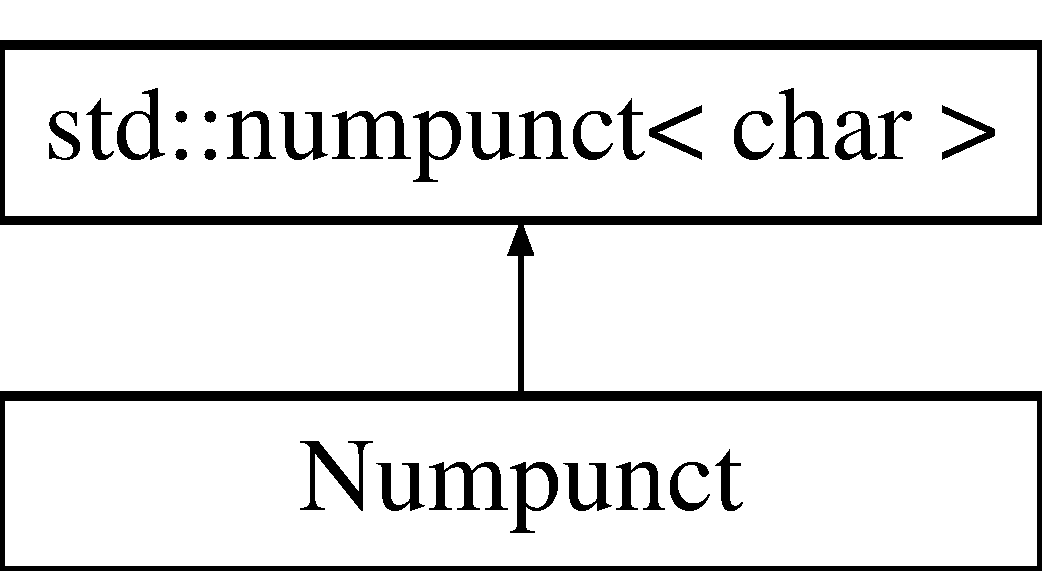
\includegraphics[height=2.000000cm]{structNumpunct}
\end{center}
\end{figure}
\subsection*{Protected Member Functions}
\begin{DoxyCompactItemize}
\item 
\mbox{\Hypertarget{structNumpunct_ab3c15bc6f961331e5ebe3657578da3a9}\label{structNumpunct_ab3c15bc6f961331e5ebe3657578da3a9}} 
virtual char {\bfseries do\+\_\+thousands\+\_\+sep} () const
\item 
\mbox{\Hypertarget{structNumpunct_a52dd791172fbb2b434f9cd9548cd1aaa}\label{structNumpunct_a52dd791172fbb2b434f9cd9548cd1aaa}} 
virtual std\+::string {\bfseries do\+\_\+grouping} () const
\end{DoxyCompactItemize}


\subsection{Detailed Description}
sturcture passed by imbue to ostreams to use commas in numbers 

The documentation for this struct was generated from the following file\+:\begin{DoxyCompactItemize}
\item 
/\+Users/jdunn/\+Documents/\+X\+Code/how\+\_\+much\+\_\+data/convolution\+\_\+test/\mbox{\hyperlink{convolution__test_8cpp}{convolution\+\_\+test.\+cpp}}\end{DoxyCompactItemize}

\hypertarget{classpareto__distribution_1_1param__type}{}\section{pareto\+\_\+distribution$<$ Real\+Type $>$\+:\+:param\+\_\+type Class Reference}
\label{classpareto__distribution_1_1param__type}\index{pareto\+\_\+distribution$<$ Real\+Type $>$\+::param\+\_\+type@{pareto\+\_\+distribution$<$ Real\+Type $>$\+::param\+\_\+type}}
\subsection*{Public Types}
\begin{DoxyCompactItemize}
\item 
\mbox{\Hypertarget{classpareto__distribution_1_1param__type_af53442713386a26de11f21594ee1a495}\label{classpareto__distribution_1_1param__type_af53442713386a26de11f21594ee1a495}} 
typedef \mbox{\hyperlink{classpareto__distribution}{pareto\+\_\+distribution}} {\bfseries distribution\+\_\+type}
\end{DoxyCompactItemize}
\subsection*{Public Member Functions}
\begin{DoxyCompactItemize}
\item 
\mbox{\hyperlink{classpareto__distribution_1_1param__type_ad7baf0b5bbef69d2ffe204e40c6db9dc}{param\+\_\+type}} (Real\+Type alpha\+\_\+arg, Real\+Type mu\+\_\+arg=Real\+Type(0.\+0), Real\+Type sigma\+\_\+arg=Real\+Type(1.\+0))
\begin{DoxyCompactList}\small\item\em Constructs the parameters of a \mbox{\hyperlink{classpareto__distribution}{pareto\+\_\+distribution}}. \end{DoxyCompactList}\item 
Real\+Type \mbox{\hyperlink{classpareto__distribution_1_1param__type_a17ac0145e5c5ba8d7b1d30686f04a8c9}{alpha}} () const
\begin{DoxyCompactList}\small\item\em Returns the \char`\"{}alpha\char`\"{} parameter of the distribution. \end{DoxyCompactList}\item 
Real\+Type \mbox{\hyperlink{classpareto__distribution_1_1param__type_a04e73cd088de22acbf0f89fdc64ffac3}{mu}} () const
\begin{DoxyCompactList}\small\item\em Returns the \char`\"{}mu\char`\"{} parameter of the distribution. \end{DoxyCompactList}\item 
Real\+Type \mbox{\hyperlink{classpareto__distribution_1_1param__type_ac115308c4703af0f20c0e3dba77ae3cb}{sigma}} () const
\begin{DoxyCompactList}\small\item\em Returns the \char`\"{}sigma\char`\"{} parameter of the distribution. \end{DoxyCompactList}\end{DoxyCompactItemize}
\subsection*{Friends}
\begin{DoxyCompactItemize}
\item 
{\footnotesize template$<$class charT , class traits $>$ }\\std\+::basic\+\_\+ostream$<$ charT, traits $>$ \& \mbox{\hyperlink{classpareto__distribution_1_1param__type_a2dfa898eef3da7b00ae3d8aaa1b8f87c}{operator$<$$<$}} (std\+::basic\+\_\+ostream$<$ charT, traits $>$ \&os, const \mbox{\hyperlink{classpareto__distribution_1_1param__type}{param\+\_\+type}} \&parm)
\begin{DoxyCompactList}\small\item\em Writes the parameters to a std\+::ostream. \end{DoxyCompactList}\item 
{\footnotesize template$<$class charT , class traits $>$ }\\std\+::basic\+\_\+istream$<$ charT, traits $>$ \& \mbox{\hyperlink{classpareto__distribution_1_1param__type_a92d697e987c5ea22b3732a535e3e922d}{operator$>$$>$}} (std\+::basic\+\_\+istream$<$ charT, traits $>$ \&is, \mbox{\hyperlink{classpareto__distribution_1_1param__type}{param\+\_\+type}} \&parm)
\begin{DoxyCompactList}\small\item\em Reads the parameters from a std\+::istream. \end{DoxyCompactList}\item 
bool \mbox{\hyperlink{classpareto__distribution_1_1param__type_ae6f3b58e629ce7a54b5e18a4f05dbc5a}{operator==}} (const \mbox{\hyperlink{classpareto__distribution_1_1param__type}{param\+\_\+type}} \&lhs, const \mbox{\hyperlink{classpareto__distribution_1_1param__type}{param\+\_\+type}} \&rhs)
\begin{DoxyCompactList}\small\item\em Returns true if the two sets of parameters are equal. \end{DoxyCompactList}\item 
bool \mbox{\hyperlink{classpareto__distribution_1_1param__type_aa559d0d98e88e84417364a89b83cf5b2}{operator!=}} (const \mbox{\hyperlink{classpareto__distribution_1_1param__type}{param\+\_\+type}} \&lhs, const \mbox{\hyperlink{classpareto__distribution_1_1param__type}{param\+\_\+type}} \&rhs)
\begin{DoxyCompactList}\small\item\em Returns true if the two sets of parameters are different. \end{DoxyCompactList}\end{DoxyCompactItemize}


\subsection{Constructor \& Destructor Documentation}
\mbox{\Hypertarget{classpareto__distribution_1_1param__type_ad7baf0b5bbef69d2ffe204e40c6db9dc}\label{classpareto__distribution_1_1param__type_ad7baf0b5bbef69d2ffe204e40c6db9dc}} 
\index{pareto\+\_\+distribution\+::param\+\_\+type@{pareto\+\_\+distribution\+::param\+\_\+type}!param\+\_\+type@{param\+\_\+type}}
\index{param\+\_\+type@{param\+\_\+type}!pareto\+\_\+distribution\+::param\+\_\+type@{pareto\+\_\+distribution\+::param\+\_\+type}}
\subsubsection{\texorpdfstring{param\+\_\+type()}{param\_type()}}
{\footnotesize\ttfamily template$<$class Real\+Type  = double$>$ \\
\mbox{\hyperlink{classpareto__distribution}{pareto\+\_\+distribution}}$<$ Real\+Type $>$\+::param\+\_\+type\+::param\+\_\+type (\begin{DoxyParamCaption}\item[{Real\+Type}]{alpha\+\_\+arg,  }\item[{Real\+Type}]{mu\+\_\+arg = {\ttfamily RealType(0.0)},  }\item[{Real\+Type}]{sigma\+\_\+arg = {\ttfamily RealType(1.0)} }\end{DoxyParamCaption})\hspace{0.3cm}{\ttfamily [inline]}, {\ttfamily [explicit]}}



Constructs the parameters of a \mbox{\hyperlink{classpareto__distribution}{pareto\+\_\+distribution}}. 



\subsection{Member Function Documentation}
\mbox{\Hypertarget{classpareto__distribution_1_1param__type_a17ac0145e5c5ba8d7b1d30686f04a8c9}\label{classpareto__distribution_1_1param__type_a17ac0145e5c5ba8d7b1d30686f04a8c9}} 
\index{pareto\+\_\+distribution\+::param\+\_\+type@{pareto\+\_\+distribution\+::param\+\_\+type}!alpha@{alpha}}
\index{alpha@{alpha}!pareto\+\_\+distribution\+::param\+\_\+type@{pareto\+\_\+distribution\+::param\+\_\+type}}
\subsubsection{\texorpdfstring{alpha()}{alpha()}}
{\footnotesize\ttfamily template$<$class Real\+Type  = double$>$ \\
Real\+Type \mbox{\hyperlink{classpareto__distribution}{pareto\+\_\+distribution}}$<$ Real\+Type $>$\+::param\+\_\+type\+::alpha (\begin{DoxyParamCaption}{ }\end{DoxyParamCaption}) const\hspace{0.3cm}{\ttfamily [inline]}}



Returns the \char`\"{}alpha\char`\"{} parameter of the distribution. 

\mbox{\Hypertarget{classpareto__distribution_1_1param__type_a04e73cd088de22acbf0f89fdc64ffac3}\label{classpareto__distribution_1_1param__type_a04e73cd088de22acbf0f89fdc64ffac3}} 
\index{pareto\+\_\+distribution\+::param\+\_\+type@{pareto\+\_\+distribution\+::param\+\_\+type}!mu@{mu}}
\index{mu@{mu}!pareto\+\_\+distribution\+::param\+\_\+type@{pareto\+\_\+distribution\+::param\+\_\+type}}
\subsubsection{\texorpdfstring{mu()}{mu()}}
{\footnotesize\ttfamily template$<$class Real\+Type  = double$>$ \\
Real\+Type \mbox{\hyperlink{classpareto__distribution}{pareto\+\_\+distribution}}$<$ Real\+Type $>$\+::param\+\_\+type\+::mu (\begin{DoxyParamCaption}{ }\end{DoxyParamCaption}) const\hspace{0.3cm}{\ttfamily [inline]}}



Returns the \char`\"{}mu\char`\"{} parameter of the distribution. 

\mbox{\Hypertarget{classpareto__distribution_1_1param__type_ac115308c4703af0f20c0e3dba77ae3cb}\label{classpareto__distribution_1_1param__type_ac115308c4703af0f20c0e3dba77ae3cb}} 
\index{pareto\+\_\+distribution\+::param\+\_\+type@{pareto\+\_\+distribution\+::param\+\_\+type}!sigma@{sigma}}
\index{sigma@{sigma}!pareto\+\_\+distribution\+::param\+\_\+type@{pareto\+\_\+distribution\+::param\+\_\+type}}
\subsubsection{\texorpdfstring{sigma()}{sigma()}}
{\footnotesize\ttfamily template$<$class Real\+Type  = double$>$ \\
Real\+Type \mbox{\hyperlink{classpareto__distribution}{pareto\+\_\+distribution}}$<$ Real\+Type $>$\+::param\+\_\+type\+::sigma (\begin{DoxyParamCaption}{ }\end{DoxyParamCaption}) const\hspace{0.3cm}{\ttfamily [inline]}}



Returns the \char`\"{}sigma\char`\"{} parameter of the distribution. 



\subsection{Friends And Related Function Documentation}
\mbox{\Hypertarget{classpareto__distribution_1_1param__type_aa559d0d98e88e84417364a89b83cf5b2}\label{classpareto__distribution_1_1param__type_aa559d0d98e88e84417364a89b83cf5b2}} 
\index{pareto\+\_\+distribution\+::param\+\_\+type@{pareto\+\_\+distribution\+::param\+\_\+type}!operator"!=@{operator"!=}}
\index{operator"!=@{operator"!=}!pareto\+\_\+distribution\+::param\+\_\+type@{pareto\+\_\+distribution\+::param\+\_\+type}}
\subsubsection{\texorpdfstring{operator"!=}{operator!=}}
{\footnotesize\ttfamily template$<$class Real\+Type  = double$>$ \\
bool operator!= (\begin{DoxyParamCaption}\item[{const \mbox{\hyperlink{classpareto__distribution_1_1param__type}{param\+\_\+type}} \&}]{lhs,  }\item[{const \mbox{\hyperlink{classpareto__distribution_1_1param__type}{param\+\_\+type}} \&}]{rhs }\end{DoxyParamCaption})\hspace{0.3cm}{\ttfamily [friend]}}



Returns true if the two sets of parameters are different. 

\mbox{\Hypertarget{classpareto__distribution_1_1param__type_a2dfa898eef3da7b00ae3d8aaa1b8f87c}\label{classpareto__distribution_1_1param__type_a2dfa898eef3da7b00ae3d8aaa1b8f87c}} 
\index{pareto\+\_\+distribution\+::param\+\_\+type@{pareto\+\_\+distribution\+::param\+\_\+type}!operator$<$$<$@{operator$<$$<$}}
\index{operator$<$$<$@{operator$<$$<$}!pareto\+\_\+distribution\+::param\+\_\+type@{pareto\+\_\+distribution\+::param\+\_\+type}}
\subsubsection{\texorpdfstring{operator$<$$<$}{operator<<}}
{\footnotesize\ttfamily template$<$class Real\+Type  = double$>$ \\
template$<$class charT , class traits $>$ \\
std\+::basic\+\_\+ostream$<$charT,traits$>$\& operator$<$$<$ (\begin{DoxyParamCaption}\item[{std\+::basic\+\_\+ostream$<$ charT, traits $>$ \&}]{os,  }\item[{const \mbox{\hyperlink{classpareto__distribution_1_1param__type}{param\+\_\+type}} \&}]{parm }\end{DoxyParamCaption})\hspace{0.3cm}{\ttfamily [friend]}}



Writes the parameters to a std\+::ostream. 

\mbox{\Hypertarget{classpareto__distribution_1_1param__type_ae6f3b58e629ce7a54b5e18a4f05dbc5a}\label{classpareto__distribution_1_1param__type_ae6f3b58e629ce7a54b5e18a4f05dbc5a}} 
\index{pareto\+\_\+distribution\+::param\+\_\+type@{pareto\+\_\+distribution\+::param\+\_\+type}!operator==@{operator==}}
\index{operator==@{operator==}!pareto\+\_\+distribution\+::param\+\_\+type@{pareto\+\_\+distribution\+::param\+\_\+type}}
\subsubsection{\texorpdfstring{operator==}{operator==}}
{\footnotesize\ttfamily template$<$class Real\+Type  = double$>$ \\
bool operator== (\begin{DoxyParamCaption}\item[{const \mbox{\hyperlink{classpareto__distribution_1_1param__type}{param\+\_\+type}} \&}]{lhs,  }\item[{const \mbox{\hyperlink{classpareto__distribution_1_1param__type}{param\+\_\+type}} \&}]{rhs }\end{DoxyParamCaption})\hspace{0.3cm}{\ttfamily [friend]}}



Returns true if the two sets of parameters are equal. 

\mbox{\Hypertarget{classpareto__distribution_1_1param__type_a92d697e987c5ea22b3732a535e3e922d}\label{classpareto__distribution_1_1param__type_a92d697e987c5ea22b3732a535e3e922d}} 
\index{pareto\+\_\+distribution\+::param\+\_\+type@{pareto\+\_\+distribution\+::param\+\_\+type}!operator$>$$>$@{operator$>$$>$}}
\index{operator$>$$>$@{operator$>$$>$}!pareto\+\_\+distribution\+::param\+\_\+type@{pareto\+\_\+distribution\+::param\+\_\+type}}
\subsubsection{\texorpdfstring{operator$>$$>$}{operator>>}}
{\footnotesize\ttfamily template$<$class Real\+Type  = double$>$ \\
template$<$class charT , class traits $>$ \\
std\+::basic\+\_\+istream$<$charT,traits$>$\& operator$>$$>$ (\begin{DoxyParamCaption}\item[{std\+::basic\+\_\+istream$<$ charT, traits $>$ \&}]{is,  }\item[{\mbox{\hyperlink{classpareto__distribution_1_1param__type}{param\+\_\+type}} \&}]{parm }\end{DoxyParamCaption})\hspace{0.3cm}{\ttfamily [friend]}}



Reads the parameters from a std\+::istream. 



The documentation for this class was generated from the following file\+:\begin{DoxyCompactItemize}
\item 
/\+Users/jdunn/\+Documents/\+X\+Code/how\+\_\+much\+\_\+data/convolution\+\_\+test/\mbox{\hyperlink{pareto__distribution_8h}{pareto\+\_\+distribution.\+h}}\end{DoxyCompactItemize}

\hypertarget{classpareto__distribution}{}\section{pareto\+\_\+distribution$<$ Real\+Type $>$ Class Template Reference}
\label{classpareto__distribution}\index{pareto\+\_\+distribution$<$ Real\+Type $>$@{pareto\+\_\+distribution$<$ Real\+Type $>$}}


Instantiations of class template \mbox{\hyperlink{classpareto__distribution}{pareto\+\_\+distribution}} model a Pareto Type 2 distribution.  




{\ttfamily \#include $<$pareto\+\_\+distribution.\+h$>$}

\subsection*{Classes}
\begin{DoxyCompactItemize}
\item 
class \mbox{\hyperlink{classpareto__distribution_1_1param__type}{param\+\_\+type}}
\end{DoxyCompactItemize}
\subsection*{Public Types}
\begin{DoxyCompactItemize}
\item 
\mbox{\Hypertarget{classpareto__distribution_ae0f18ad8753167df9c0acfe79578913e}\label{classpareto__distribution_ae0f18ad8753167df9c0acfe79578913e}} 
typedef Real\+Type {\bfseries result\+\_\+type}
\end{DoxyCompactItemize}
\subsection*{Public Member Functions}
\begin{DoxyCompactItemize}
\item 
\mbox{\hyperlink{classpareto__distribution_a667f195859ce355378510b79c2a6e6ee}{pareto\+\_\+distribution}} (Real\+Type alpha\+\_\+arg, Real\+Type mu\+\_\+arg=Real\+Type(0.\+0), Real\+Type sigma\+\_\+arg=Real\+Type(1.\+0))
\begin{DoxyCompactList}\small\item\em Constructs a \mbox{\hyperlink{classpareto__distribution}{pareto\+\_\+distribution}}. \end{DoxyCompactList}\item 
\mbox{\Hypertarget{classpareto__distribution_ad08df2fa3ced8fec377e35fa9ded260b}\label{classpareto__distribution_ad08df2fa3ced8fec377e35fa9ded260b}} 
\mbox{\hyperlink{classpareto__distribution_ad08df2fa3ced8fec377e35fa9ded260b}{pareto\+\_\+distribution}} (const \mbox{\hyperlink{classpareto__distribution_1_1param__type}{param\+\_\+type}} \&parm)
\begin{DoxyCompactList}\small\item\em Constructs a \mbox{\hyperlink{classpareto__distribution}{pareto\+\_\+distribution}} from its parameters. \end{DoxyCompactList}\item 
Real\+Type \mbox{\hyperlink{classpareto__distribution_a4e867e8f34f77a9953873987374fb5d0}{alpha}} () const
\begin{DoxyCompactList}\small\item\em Returns the alpha parameter of the distribution. \end{DoxyCompactList}\item 
Real\+Type \mbox{\hyperlink{classpareto__distribution_ab4fd822cde4f415efa8e0bc6ce7c2bad}{mu}} () const
\begin{DoxyCompactList}\small\item\em Returns the mu parameter of the distribution. \end{DoxyCompactList}\item 
Real\+Type \mbox{\hyperlink{classpareto__distribution_a739d59031c3fd72af690ec68c1073afc}{sigma}} () const
\begin{DoxyCompactList}\small\item\em Returns the sigma parameter of the distribution. \end{DoxyCompactList}\item 
\mbox{\Hypertarget{classpareto__distribution_a6b9aed9573f877b6d7e84c109f443a40}\label{classpareto__distribution_a6b9aed9573f877b6d7e84c109f443a40}} 
Real\+Type \mbox{\hyperlink{classpareto__distribution_a6b9aed9573f877b6d7e84c109f443a40}{alpha\+\_\+stable}} () const
\begin{DoxyCompactList}\small\item\em Return the alpha of the asymptotic stable distribution. \end{DoxyCompactList}\item 
Real\+Type \mbox{\hyperlink{classpareto__distribution_a73ccdc7f9a3f3131d58627a94789ecfb}{min}} () const
\begin{DoxyCompactList}\small\item\em Returns the smallest value that the distribution can produce. \end{DoxyCompactList}\item 
Real\+Type \mbox{\hyperlink{classpareto__distribution_a884ff35d4c1d1b5979e17c8eee41f397}{max}} () const
\begin{DoxyCompactList}\small\item\em Returns the largest value that the distribution can produce. \end{DoxyCompactList}\item 
\mbox{\hyperlink{classpareto__distribution_1_1param__type}{param\+\_\+type}} \mbox{\hyperlink{classpareto__distribution_ae56d30e604eb00dd286f99cdf6764bda}{param}} () const
\begin{DoxyCompactList}\small\item\em Returns the parameters of the distribution. \end{DoxyCompactList}\item 
void \mbox{\hyperlink{classpareto__distribution_aea6ab161e197e7350f5477492d00fe59}{param}} (const \mbox{\hyperlink{classpareto__distribution_1_1param__type}{param\+\_\+type}} \&parm)
\begin{DoxyCompactList}\small\item\em Sets the parameters of the distribution. \end{DoxyCompactList}\item 
\mbox{\Hypertarget{classpareto__distribution_a6526c615f4ebcb26f1c88728d99db2d8}\label{classpareto__distribution_a6526c615f4ebcb26f1c88728d99db2d8}} 
Real\+Type \mbox{\hyperlink{classpareto__distribution_a6526c615f4ebcb26f1c88728d99db2d8}{cdf}} (Real\+Type x, bool lower\+\_\+tail=true) const
\begin{DoxyCompactList}\small\item\em the cdf of the distribution \end{DoxyCompactList}\item 
\mbox{\Hypertarget{classpareto__distribution_a8cb3ee0a57c036cd9caecf515db32319}\label{classpareto__distribution_a8cb3ee0a57c036cd9caecf515db32319}} 
Real\+Type \mbox{\hyperlink{classpareto__distribution_a8cb3ee0a57c036cd9caecf515db32319}{pdf}} (Real\+Type x) const
\begin{DoxyCompactList}\small\item\em return the pdf of the distribution \end{DoxyCompactList}\item 
\mbox{\Hypertarget{classpareto__distribution_a970d489ff62a6da2bdef99e0bf82461b}\label{classpareto__distribution_a970d489ff62a6da2bdef99e0bf82461b}} 
Real\+Type \mbox{\hyperlink{classpareto__distribution_a970d489ff62a6da2bdef99e0bf82461b}{quantile}} (Real\+Type p) const
\begin{DoxyCompactList}\small\item\em the quantile for a given probability \end{DoxyCompactList}\item 
\mbox{\Hypertarget{classpareto__distribution_a5951ce961898e3c1b82dc5a17eb2b1e6}\label{classpareto__distribution_a5951ce961898e3c1b82dc5a17eb2b1e6}} 
Real\+Type \mbox{\hyperlink{classpareto__distribution_a5951ce961898e3c1b82dc5a17eb2b1e6}{mean}} () const
\begin{DoxyCompactList}\small\item\em Return the mean of the distribution. \end{DoxyCompactList}\item 
\mbox{\Hypertarget{classpareto__distribution_a18178125ec26f855f5a1b9e5bb1b38e2}\label{classpareto__distribution_a18178125ec26f855f5a1b9e5bb1b38e2}} 
Real\+Type \mbox{\hyperlink{classpareto__distribution_a18178125ec26f855f5a1b9e5bb1b38e2}{mad}} () const
\begin{DoxyCompactList}\small\item\em Return the M\+AD of the distribution. \end{DoxyCompactList}\item 
\mbox{\Hypertarget{classpareto__distribution_ae7a0e96cb0dc175cb7f82aa231f801f2}\label{classpareto__distribution_ae7a0e96cb0dc175cb7f82aa231f801f2}} 
Real\+Type \mbox{\hyperlink{classpareto__distribution_ae7a0e96cb0dc175cb7f82aa231f801f2}{mad2}} () const
\begin{DoxyCompactList}\small\item\em Return the M\+AD of the square of the distribution. \end{DoxyCompactList}\item 
\mbox{\Hypertarget{classpareto__distribution_acef7b13822b8ea6489c01d43bb71caf9}\label{classpareto__distribution_acef7b13822b8ea6489c01d43bb71caf9}} 
complex$<$ Real\+Type $>$ \mbox{\hyperlink{classpareto__distribution_acef7b13822b8ea6489c01d43bb71caf9}{characteristic\+\_\+function}} (Real\+Type omega) const
\begin{DoxyCompactList}\small\item\em return the characteristic function of the distribution \end{DoxyCompactList}\item 
\mbox{\Hypertarget{classpareto__distribution_a16760711aa205086d54b08c601c39fac}\label{classpareto__distribution_a16760711aa205086d54b08c601c39fac}} 
complex$<$ Real\+Type $>$ \mbox{\hyperlink{classpareto__distribution_a16760711aa205086d54b08c601c39fac}{characteristic\+\_\+function}} (complex$<$ Real\+Type $>$ omega) const
\begin{DoxyCompactList}\small\item\em return the characteristic function of the distribution given complex argument \end{DoxyCompactList}\item 
\mbox{\Hypertarget{classpareto__distribution_a3e0c538acff3b7ae2b122cd23d8921fa}\label{classpareto__distribution_a3e0c538acff3b7ae2b122cd23d8921fa}} 
complex$<$ Real\+Type $>$ \mbox{\hyperlink{classpareto__distribution_a3e0c538acff3b7ae2b122cd23d8921fa}{characteristic\+\_\+function\+\_\+prime}} (Real\+Type omega) const
\begin{DoxyCompactList}\small\item\em return the derivative of th characteristic function of the distribution \end{DoxyCompactList}\item 
\mbox{\Hypertarget{classpareto__distribution_ac04f96a919fa7096369301605749c1fa}\label{classpareto__distribution_ac04f96a919fa7096369301605749c1fa}} 
complex$<$ Real\+Type $>$ \mbox{\hyperlink{classpareto__distribution_ac04f96a919fa7096369301605749c1fa}{characteristic\+\_\+function\+\_\+prime}} (complex$<$ Real\+Type $>$ omega) const
\begin{DoxyCompactList}\small\item\em return the derivative of th char. fnct. of the dist. given complex arg. \end{DoxyCompactList}\item 
\mbox{\Hypertarget{classpareto__distribution_a0ab5bbfc1834d4184db153a5803922eb}\label{classpareto__distribution_a0ab5bbfc1834d4184db153a5803922eb}} 
Real\+Type \mbox{\hyperlink{classpareto__distribution_a0ab5bbfc1834d4184db153a5803922eb}{ci}} (Real\+Type level=Real\+Type(.\+05)) const
\begin{DoxyCompactList}\small\item\em Return the 95\% confidence interval. \end{DoxyCompactList}\item 
\mbox{\Hypertarget{classpareto__distribution_afaf787428998d91ac739d2a5356f3e20}\label{classpareto__distribution_afaf787428998d91ac739d2a5356f3e20}} 
void \mbox{\hyperlink{classpareto__distribution_afaf787428998d91ac739d2a5356f3e20}{reset}} ()
\begin{DoxyCompactList}\small\item\em Effects\+: Subsequent uses of the distribution do not depend on values produced by any engine prior to invoking reset. \end{DoxyCompactList}\item 
\mbox{\Hypertarget{classpareto__distribution_ad711d059b455b643767fb9e907595d67}\label{classpareto__distribution_ad711d059b455b643767fb9e907595d67}} 
{\footnotesize template$<$class Engine $>$ }\\result\+\_\+type \mbox{\hyperlink{classpareto__distribution_ad711d059b455b643767fb9e907595d67}{operator()}} (Engine \&eng) const
\begin{DoxyCompactList}\small\item\em Returns a random variate distributed according to the Pareto distribution. \end{DoxyCompactList}\item 
\mbox{\Hypertarget{classpareto__distribution_a627683402f68bba682621994612d9f28}\label{classpareto__distribution_a627683402f68bba682621994612d9f28}} 
{\footnotesize template$<$class Engine $>$ }\\result\+\_\+type \mbox{\hyperlink{classpareto__distribution_a627683402f68bba682621994612d9f28}{operator()}} (Engine \&eng, const \mbox{\hyperlink{classpareto__distribution_1_1param__type}{param\+\_\+type}} \&parm)
\begin{DoxyCompactList}\small\item\em Returns a random variate distributed according to the Pareto distribution with parameters specified by param. \end{DoxyCompactList}\end{DoxyCompactItemize}
\subsection*{Friends}
\begin{DoxyCompactItemize}
\item 
\mbox{\Hypertarget{classpareto__distribution_a3edbe39cc0f6942c0b3852fac6d416d9}\label{classpareto__distribution_a3edbe39cc0f6942c0b3852fac6d416d9}} 
{\footnotesize template$<$class charT , class traits $>$ }\\std\+::basic\+\_\+ostream$<$ charT, traits $>$ \& \mbox{\hyperlink{classpareto__distribution_a3edbe39cc0f6942c0b3852fac6d416d9}{operator$<$$<$}} (std\+::basic\+\_\+ostream$<$ charT, traits $>$ \&os, const \mbox{\hyperlink{classpareto__distribution}{pareto\+\_\+distribution}} \&dist)
\begin{DoxyCompactList}\small\item\em Write distribution to std\+::ostream. \end{DoxyCompactList}\item 
{\footnotesize template$<$class charT , class traits $>$ }\\std\+::basic\+\_\+istream$<$ charT, traits $>$ \& \mbox{\hyperlink{classpareto__distribution_a827211558343a83cda447b5ab8cce83a}{operator$>$$>$}} (std\+::basic\+\_\+istream$<$ charT, traits $>$ \&is, \mbox{\hyperlink{classpareto__distribution}{pareto\+\_\+distribution}} \&dist)
\begin{DoxyCompactList}\small\item\em Reads the parameters from a std\+::istream. \end{DoxyCompactList}\item 
\mbox{\Hypertarget{classpareto__distribution_a7a67a2ffe5fc96ec9d485f5b33c6d1b6}\label{classpareto__distribution_a7a67a2ffe5fc96ec9d485f5b33c6d1b6}} 
bool \mbox{\hyperlink{classpareto__distribution_a7a67a2ffe5fc96ec9d485f5b33c6d1b6}{operator==}} (const \mbox{\hyperlink{classpareto__distribution}{pareto\+\_\+distribution}} \&lhs, const \mbox{\hyperlink{classpareto__distribution}{pareto\+\_\+distribution}} \&rhs)
\begin{DoxyCompactList}\small\item\em Returns true if the two distributions will produce identical sequences of values given equal generators. \end{DoxyCompactList}\item 
\mbox{\Hypertarget{classpareto__distribution_a77e9e309508a372c4bf25a0338513cfc}\label{classpareto__distribution_a77e9e309508a372c4bf25a0338513cfc}} 
bool \mbox{\hyperlink{classpareto__distribution_a77e9e309508a372c4bf25a0338513cfc}{operator!=}} (const \mbox{\hyperlink{classpareto__distribution}{pareto\+\_\+distribution}} \&lhs, const \mbox{\hyperlink{classpareto__distribution}{pareto\+\_\+distribution}} \&rhs)
\begin{DoxyCompactList}\small\item\em Returns true if the two distributions may produce different sequences of values given equal generators. \end{DoxyCompactList}\end{DoxyCompactItemize}


\subsection{Detailed Description}
\subsubsection*{template$<$class Real\+Type = double$>$\newline
class pareto\+\_\+distribution$<$ Real\+Type $>$}

Instantiations of class template \mbox{\hyperlink{classpareto__distribution}{pareto\+\_\+distribution}} model a Pareto Type 2 distribution. 

Such a distribution produces random numbers with $\displaystyle 1-F(x) = (1+\frac{x-\mu}{\sigma})^{-\alpha}$ for $ x > \mu $. 

\subsection{Constructor \& Destructor Documentation}
\mbox{\Hypertarget{classpareto__distribution_a667f195859ce355378510b79c2a6e6ee}\label{classpareto__distribution_a667f195859ce355378510b79c2a6e6ee}} 
\index{pareto\+\_\+distribution@{pareto\+\_\+distribution}!pareto\+\_\+distribution@{pareto\+\_\+distribution}}
\index{pareto\+\_\+distribution@{pareto\+\_\+distribution}!pareto\+\_\+distribution@{pareto\+\_\+distribution}}
\subsubsection{\texorpdfstring{pareto\+\_\+distribution()}{pareto\_distribution()}}
{\footnotesize\ttfamily template$<$class Real\+Type  = double$>$ \\
\mbox{\hyperlink{classpareto__distribution}{pareto\+\_\+distribution}}$<$ Real\+Type $>$\+::\mbox{\hyperlink{classpareto__distribution}{pareto\+\_\+distribution}} (\begin{DoxyParamCaption}\item[{Real\+Type}]{alpha\+\_\+arg,  }\item[{Real\+Type}]{mu\+\_\+arg = {\ttfamily RealType(0.0)},  }\item[{Real\+Type}]{sigma\+\_\+arg = {\ttfamily RealType(1.0)} }\end{DoxyParamCaption})\hspace{0.3cm}{\ttfamily [inline]}, {\ttfamily [explicit]}}



Constructs a \mbox{\hyperlink{classpareto__distribution}{pareto\+\_\+distribution}}. 

{\ttfamily alpha} {\ttfamily mu} and {\ttfamily sigma} are the parameters of the distribution. 

\subsection{Member Function Documentation}
\mbox{\Hypertarget{classpareto__distribution_a4e867e8f34f77a9953873987374fb5d0}\label{classpareto__distribution_a4e867e8f34f77a9953873987374fb5d0}} 
\index{pareto\+\_\+distribution@{pareto\+\_\+distribution}!alpha@{alpha}}
\index{alpha@{alpha}!pareto\+\_\+distribution@{pareto\+\_\+distribution}}
\subsubsection{\texorpdfstring{alpha()}{alpha()}}
{\footnotesize\ttfamily template$<$class Real\+Type  = double$>$ \\
Real\+Type \mbox{\hyperlink{classpareto__distribution}{pareto\+\_\+distribution}}$<$ Real\+Type $>$\+::alpha (\begin{DoxyParamCaption}{ }\end{DoxyParamCaption}) const\hspace{0.3cm}{\ttfamily [inline]}}



Returns the alpha parameter of the distribution. 

\mbox{\Hypertarget{classpareto__distribution_a884ff35d4c1d1b5979e17c8eee41f397}\label{classpareto__distribution_a884ff35d4c1d1b5979e17c8eee41f397}} 
\index{pareto\+\_\+distribution@{pareto\+\_\+distribution}!max@{max}}
\index{max@{max}!pareto\+\_\+distribution@{pareto\+\_\+distribution}}
\subsubsection{\texorpdfstring{max()}{max()}}
{\footnotesize\ttfamily template$<$class Real\+Type  = double$>$ \\
Real\+Type \mbox{\hyperlink{classpareto__distribution}{pareto\+\_\+distribution}}$<$ Real\+Type $>$\+::max (\begin{DoxyParamCaption}{ }\end{DoxyParamCaption}) const\hspace{0.3cm}{\ttfamily [inline]}}



Returns the largest value that the distribution can produce. 

\mbox{\Hypertarget{classpareto__distribution_a73ccdc7f9a3f3131d58627a94789ecfb}\label{classpareto__distribution_a73ccdc7f9a3f3131d58627a94789ecfb}} 
\index{pareto\+\_\+distribution@{pareto\+\_\+distribution}!min@{min}}
\index{min@{min}!pareto\+\_\+distribution@{pareto\+\_\+distribution}}
\subsubsection{\texorpdfstring{min()}{min()}}
{\footnotesize\ttfamily template$<$class Real\+Type  = double$>$ \\
Real\+Type \mbox{\hyperlink{classpareto__distribution}{pareto\+\_\+distribution}}$<$ Real\+Type $>$\+::min (\begin{DoxyParamCaption}{ }\end{DoxyParamCaption}) const\hspace{0.3cm}{\ttfamily [inline]}}



Returns the smallest value that the distribution can produce. 

\mbox{\Hypertarget{classpareto__distribution_ab4fd822cde4f415efa8e0bc6ce7c2bad}\label{classpareto__distribution_ab4fd822cde4f415efa8e0bc6ce7c2bad}} 
\index{pareto\+\_\+distribution@{pareto\+\_\+distribution}!mu@{mu}}
\index{mu@{mu}!pareto\+\_\+distribution@{pareto\+\_\+distribution}}
\subsubsection{\texorpdfstring{mu()}{mu()}}
{\footnotesize\ttfamily template$<$class Real\+Type  = double$>$ \\
Real\+Type \mbox{\hyperlink{classpareto__distribution}{pareto\+\_\+distribution}}$<$ Real\+Type $>$\+::mu (\begin{DoxyParamCaption}{ }\end{DoxyParamCaption}) const\hspace{0.3cm}{\ttfamily [inline]}}



Returns the mu parameter of the distribution. 

\mbox{\Hypertarget{classpareto__distribution_ae56d30e604eb00dd286f99cdf6764bda}\label{classpareto__distribution_ae56d30e604eb00dd286f99cdf6764bda}} 
\index{pareto\+\_\+distribution@{pareto\+\_\+distribution}!param@{param}}
\index{param@{param}!pareto\+\_\+distribution@{pareto\+\_\+distribution}}
\subsubsection{\texorpdfstring{param()}{param()}\hspace{0.1cm}{\footnotesize\ttfamily [1/2]}}
{\footnotesize\ttfamily template$<$class Real\+Type  = double$>$ \\
\mbox{\hyperlink{classpareto__distribution_1_1param__type}{param\+\_\+type}} \mbox{\hyperlink{classpareto__distribution}{pareto\+\_\+distribution}}$<$ Real\+Type $>$\+::param (\begin{DoxyParamCaption}{ }\end{DoxyParamCaption}) const\hspace{0.3cm}{\ttfamily [inline]}}



Returns the parameters of the distribution. 

\mbox{\Hypertarget{classpareto__distribution_aea6ab161e197e7350f5477492d00fe59}\label{classpareto__distribution_aea6ab161e197e7350f5477492d00fe59}} 
\index{pareto\+\_\+distribution@{pareto\+\_\+distribution}!param@{param}}
\index{param@{param}!pareto\+\_\+distribution@{pareto\+\_\+distribution}}
\subsubsection{\texorpdfstring{param()}{param()}\hspace{0.1cm}{\footnotesize\ttfamily [2/2]}}
{\footnotesize\ttfamily template$<$class Real\+Type  = double$>$ \\
void \mbox{\hyperlink{classpareto__distribution}{pareto\+\_\+distribution}}$<$ Real\+Type $>$\+::param (\begin{DoxyParamCaption}\item[{const \mbox{\hyperlink{classpareto__distribution_1_1param__type}{param\+\_\+type}} \&}]{parm }\end{DoxyParamCaption})\hspace{0.3cm}{\ttfamily [inline]}}



Sets the parameters of the distribution. 

\mbox{\Hypertarget{classpareto__distribution_a739d59031c3fd72af690ec68c1073afc}\label{classpareto__distribution_a739d59031c3fd72af690ec68c1073afc}} 
\index{pareto\+\_\+distribution@{pareto\+\_\+distribution}!sigma@{sigma}}
\index{sigma@{sigma}!pareto\+\_\+distribution@{pareto\+\_\+distribution}}
\subsubsection{\texorpdfstring{sigma()}{sigma()}}
{\footnotesize\ttfamily template$<$class Real\+Type  = double$>$ \\
Real\+Type \mbox{\hyperlink{classpareto__distribution}{pareto\+\_\+distribution}}$<$ Real\+Type $>$\+::sigma (\begin{DoxyParamCaption}{ }\end{DoxyParamCaption}) const\hspace{0.3cm}{\ttfamily [inline]}}



Returns the sigma parameter of the distribution. 



\subsection{Friends And Related Function Documentation}
\mbox{\Hypertarget{classpareto__distribution_a827211558343a83cda447b5ab8cce83a}\label{classpareto__distribution_a827211558343a83cda447b5ab8cce83a}} 
\index{pareto\+\_\+distribution@{pareto\+\_\+distribution}!operator$>$$>$@{operator$>$$>$}}
\index{operator$>$$>$@{operator$>$$>$}!pareto\+\_\+distribution@{pareto\+\_\+distribution}}
\subsubsection{\texorpdfstring{operator$>$$>$}{operator>>}}
{\footnotesize\ttfamily template$<$class Real\+Type  = double$>$ \\
template$<$class charT , class traits $>$ \\
std\+::basic\+\_\+istream$<$charT,traits$>$\& operator$>$$>$ (\begin{DoxyParamCaption}\item[{std\+::basic\+\_\+istream$<$ charT, traits $>$ \&}]{is,  }\item[{\mbox{\hyperlink{classpareto__distribution}{pareto\+\_\+distribution}}$<$ Real\+Type $>$ \&}]{dist }\end{DoxyParamCaption})\hspace{0.3cm}{\ttfamily [friend]}}



Reads the parameters from a std\+::istream. 



The documentation for this class was generated from the following file\+:\begin{DoxyCompactItemize}
\item 
/\+Users/jdunn/\+Documents/\+X\+Code/how\+\_\+much\+\_\+data/include/\mbox{\hyperlink{pareto__distribution_8h}{pareto\+\_\+distribution.\+h}}\end{DoxyCompactItemize}

\hypertarget{classPinelisTalebIntegrand}{}\section{Pinelis\+Taleb\+Integrand$<$ Dist $>$ Class Template Reference}
\label{classPinelisTalebIntegrand}\index{Pinelis\+Taleb\+Integrand$<$ Dist $>$@{Pinelis\+Taleb\+Integrand$<$ Dist $>$}}


Functor used in the integratoin of the Pinelis Taleb result.  


\subsection*{Public Member Functions}
\begin{DoxyCompactItemize}
\item 
\mbox{\hyperlink{classPinelisTalebIntegrand_a4122d67af083c9b7f38cc94ed85e99f7}{Pinelis\+Taleb\+Integrand}} (Dist \&dist, const int n)
\begin{DoxyCompactList}\small\item\em construct the integrand \end{DoxyCompactList}\item 
\mbox{\Hypertarget{classPinelisTalebIntegrand_a065e7c917d79d417efaf2185a343031d}\label{classPinelisTalebIntegrand_a065e7c917d79d417efaf2185a343031d}} 
double \mbox{\hyperlink{classPinelisTalebIntegrand_a065e7c917d79d417efaf2185a343031d}{operator()}} (double x)
\begin{DoxyCompactList}\small\item\em return the value of the Pinelis Taleb integrand \end{DoxyCompactList}\item 
\mbox{\Hypertarget{classPinelisTalebIntegrand_a2c46e6c2f8b63b6deb45b8be5c1b81e5}\label{classPinelisTalebIntegrand_a2c46e6c2f8b63b6deb45b8be5c1b81e5}} 
void {\bfseries operator()} (std\+::vector$<$ double $>$ \&xs)
\end{DoxyCompactItemize}


\subsection{Detailed Description}
\subsubsection*{template$<$typename Dist$>$\newline
class Pinelis\+Taleb\+Integrand$<$ Dist $>$}

Functor used in the integratoin of the Pinelis Taleb result. 

\subsection{Constructor \& Destructor Documentation}
\mbox{\Hypertarget{classPinelisTalebIntegrand_a4122d67af083c9b7f38cc94ed85e99f7}\label{classPinelisTalebIntegrand_a4122d67af083c9b7f38cc94ed85e99f7}} 
\index{Pinelis\+Taleb\+Integrand@{Pinelis\+Taleb\+Integrand}!Pinelis\+Taleb\+Integrand@{Pinelis\+Taleb\+Integrand}}
\index{Pinelis\+Taleb\+Integrand@{Pinelis\+Taleb\+Integrand}!Pinelis\+Taleb\+Integrand@{Pinelis\+Taleb\+Integrand}}
\subsubsection{\texorpdfstring{Pinelis\+Taleb\+Integrand()}{PinelisTalebIntegrand()}}
{\footnotesize\ttfamily template$<$typename Dist $>$ \\
\mbox{\hyperlink{classPinelisTalebIntegrand}{Pinelis\+Taleb\+Integrand}}$<$ Dist $>$\+::\mbox{\hyperlink{classPinelisTalebIntegrand}{Pinelis\+Taleb\+Integrand}} (\begin{DoxyParamCaption}\item[{Dist \&}]{dist,  }\item[{const int}]{n }\end{DoxyParamCaption})\hspace{0.3cm}{\ttfamily [inline]}}



construct the integrand 


\begin{DoxyParams}[1]{Parameters}
\mbox{\tt in}  & {\em dist} & the distribution \\
\hline
\mbox{\tt in}  & {\em n} & the duration \\
\hline
\end{DoxyParams}


The documentation for this class was generated from the following file\+:\begin{DoxyCompactItemize}
\item 
/\+Users/jdunn/\+Documents/\+X\+Code/how\+\_\+much\+\_\+data/pinelis\+\_\+taleb\+\_\+test/\mbox{\hyperlink{pinelis__taleb__test_8cpp}{pinelis\+\_\+taleb\+\_\+test.\+cpp}}\end{DoxyCompactItemize}

\hypertarget{classPinelisTalebIntegrand_3_01exponential__distribution_3_4_01_4}{}\section{Pinelis\+Taleb\+Integrand$<$ exponential\+\_\+distribution$<$$>$ $>$ Class Template Reference}
\label{classPinelisTalebIntegrand_3_01exponential__distribution_3_4_01_4}\index{Pinelis\+Taleb\+Integrand$<$ exponential\+\_\+distribution$<$$>$ $>$@{Pinelis\+Taleb\+Integrand$<$ exponential\+\_\+distribution$<$$>$ $>$}}


Functor used in the integration of the Pinelis Taleb result for exp. dist.  


\subsection*{Public Member Functions}
\begin{DoxyCompactItemize}
\item 
\mbox{\hyperlink{classPinelisTalebIntegrand_3_01exponential__distribution_3_4_01_4_acf3ed4eb347c425dfd458300ac1e717a}{Pinelis\+Taleb\+Integrand}} (const \mbox{\hyperlink{structexponential__distribution}{exponential\+\_\+distribution}}$<$$>$ \&dist, const int n)
\begin{DoxyCompactList}\small\item\em construct the integrand \end{DoxyCompactList}\item 
\mbox{\Hypertarget{classPinelisTalebIntegrand_3_01exponential__distribution_3_4_01_4_a5a1d91c7452d9590e85d772fb68d2298}\label{classPinelisTalebIntegrand_3_01exponential__distribution_3_4_01_4_a5a1d91c7452d9590e85d772fb68d2298}} 
double \mbox{\hyperlink{classPinelisTalebIntegrand_3_01exponential__distribution_3_4_01_4_a5a1d91c7452d9590e85d772fb68d2298}{operator()}} (double x) const
\begin{DoxyCompactList}\small\item\em return the value of the Pinelis Taleb integrand for exp distribution Uses an adjusted contour of integration \end{DoxyCompactList}\item 
\mbox{\Hypertarget{classPinelisTalebIntegrand_3_01exponential__distribution_3_4_01_4_a66aef8eefd6f272f6f2cdea0462c66e5}\label{classPinelisTalebIntegrand_3_01exponential__distribution_3_4_01_4_a66aef8eefd6f272f6f2cdea0462c66e5}} 
void {\bfseries operator()} (std\+::vector$<$ double $>$ \&xs) const
\end{DoxyCompactItemize}


\subsection{Detailed Description}
\subsubsection*{template$<$$>$\newline
class Pinelis\+Taleb\+Integrand$<$ exponential\+\_\+distribution$<$$>$ $>$}

Functor used in the integration of the Pinelis Taleb result for exp. dist. 

\subsection{Constructor \& Destructor Documentation}
\mbox{\Hypertarget{classPinelisTalebIntegrand_3_01exponential__distribution_3_4_01_4_acf3ed4eb347c425dfd458300ac1e717a}\label{classPinelisTalebIntegrand_3_01exponential__distribution_3_4_01_4_acf3ed4eb347c425dfd458300ac1e717a}} 
\index{Pinelis\+Taleb\+Integrand$<$ exponential\+\_\+distribution$<$$>$ $>$@{Pinelis\+Taleb\+Integrand$<$ exponential\+\_\+distribution$<$$>$ $>$}!Pinelis\+Taleb\+Integrand@{Pinelis\+Taleb\+Integrand}}
\index{Pinelis\+Taleb\+Integrand@{Pinelis\+Taleb\+Integrand}!Pinelis\+Taleb\+Integrand$<$ exponential\+\_\+distribution$<$$>$ $>$@{Pinelis\+Taleb\+Integrand$<$ exponential\+\_\+distribution$<$$>$ $>$}}
\subsubsection{\texorpdfstring{Pinelis\+Taleb\+Integrand()}{PinelisTalebIntegrand()}}
{\footnotesize\ttfamily \mbox{\hyperlink{classPinelisTalebIntegrand}{Pinelis\+Taleb\+Integrand}}$<$ \mbox{\hyperlink{structexponential__distribution}{exponential\+\_\+distribution}}$<$$>$ $>$\+::\mbox{\hyperlink{classPinelisTalebIntegrand}{Pinelis\+Taleb\+Integrand}} (\begin{DoxyParamCaption}\item[{const \mbox{\hyperlink{structexponential__distribution}{exponential\+\_\+distribution}}$<$$>$ \&}]{dist,  }\item[{const int}]{n }\end{DoxyParamCaption})\hspace{0.3cm}{\ttfamily [inline]}}



construct the integrand 


\begin{DoxyParams}[1]{Parameters}
\mbox{\tt in}  & {\em dist} & the distribution \\
\hline
\mbox{\tt in}  & {\em n} & the duration \\
\hline
\end{DoxyParams}


The documentation for this class was generated from the following file\+:\begin{DoxyCompactItemize}
\item 
/\+Users/jdunn/\+Documents/\+X\+Code/how\+\_\+much\+\_\+data/pinelis\+\_\+taleb\+\_\+test/\mbox{\hyperlink{pinelis__taleb__test_8cpp}{pinelis\+\_\+taleb\+\_\+test.\+cpp}}\end{DoxyCompactItemize}

\hypertarget{classPinelisTalebIntegrand_3_01pareto__distribution_3_4_01_4}{}\section{Pinelis\+Taleb\+Integrand$<$ pareto\+\_\+distribution$<$$>$ $>$ Class Template Reference}
\label{classPinelisTalebIntegrand_3_01pareto__distribution_3_4_01_4}\index{Pinelis\+Taleb\+Integrand$<$ pareto\+\_\+distribution$<$$>$ $>$@{Pinelis\+Taleb\+Integrand$<$ pareto\+\_\+distribution$<$$>$ $>$}}


Functor used in the integration of the Pinelis Taleb result for pareto dist.  


\subsection*{Public Member Functions}
\begin{DoxyCompactItemize}
\item 
\mbox{\hyperlink{classPinelisTalebIntegrand_3_01pareto__distribution_3_4_01_4_a518cd7558e51a20773b82d71b5eaa817}{Pinelis\+Taleb\+Integrand}} (\mbox{\hyperlink{classpareto__distribution}{pareto\+\_\+distribution}}$<$$>$ \&dist, const int n)
\begin{DoxyCompactList}\small\item\em construct the integrand \end{DoxyCompactList}\item 
\mbox{\Hypertarget{classPinelisTalebIntegrand_3_01pareto__distribution_3_4_01_4_ae542b541e99e72c6e22c1a69cbc4abfa}\label{classPinelisTalebIntegrand_3_01pareto__distribution_3_4_01_4_ae542b541e99e72c6e22c1a69cbc4abfa}} 
double \mbox{\hyperlink{classPinelisTalebIntegrand_3_01pareto__distribution_3_4_01_4_ae542b541e99e72c6e22c1a69cbc4abfa}{operator()}} (double x) const
\begin{DoxyCompactList}\small\item\em return the value of the Pinelis Taleb integrand for pareto distribution Uses an adjusted contour of integration \end{DoxyCompactList}\item 
\mbox{\Hypertarget{classPinelisTalebIntegrand_3_01pareto__distribution_3_4_01_4_a103c4b234553d169a2ee69f7e6ba5804}\label{classPinelisTalebIntegrand_3_01pareto__distribution_3_4_01_4_a103c4b234553d169a2ee69f7e6ba5804}} 
void {\bfseries operator()} (std\+::vector$<$ double $>$ \&xs) const
\end{DoxyCompactItemize}


\subsection{Detailed Description}
\subsubsection*{template$<$$>$\newline
class Pinelis\+Taleb\+Integrand$<$ pareto\+\_\+distribution$<$$>$ $>$}

Functor used in the integration of the Pinelis Taleb result for pareto dist. 

\subsection{Constructor \& Destructor Documentation}
\mbox{\Hypertarget{classPinelisTalebIntegrand_3_01pareto__distribution_3_4_01_4_a518cd7558e51a20773b82d71b5eaa817}\label{classPinelisTalebIntegrand_3_01pareto__distribution_3_4_01_4_a518cd7558e51a20773b82d71b5eaa817}} 
\index{Pinelis\+Taleb\+Integrand$<$ pareto\+\_\+distribution$<$$>$ $>$@{Pinelis\+Taleb\+Integrand$<$ pareto\+\_\+distribution$<$$>$ $>$}!Pinelis\+Taleb\+Integrand@{Pinelis\+Taleb\+Integrand}}
\index{Pinelis\+Taleb\+Integrand@{Pinelis\+Taleb\+Integrand}!Pinelis\+Taleb\+Integrand$<$ pareto\+\_\+distribution$<$$>$ $>$@{Pinelis\+Taleb\+Integrand$<$ pareto\+\_\+distribution$<$$>$ $>$}}
\subsubsection{\texorpdfstring{Pinelis\+Taleb\+Integrand()}{PinelisTalebIntegrand()}}
{\footnotesize\ttfamily \mbox{\hyperlink{classPinelisTalebIntegrand}{Pinelis\+Taleb\+Integrand}}$<$ \mbox{\hyperlink{classpareto__distribution}{pareto\+\_\+distribution}}$<$$>$ $>$\+::\mbox{\hyperlink{classPinelisTalebIntegrand}{Pinelis\+Taleb\+Integrand}} (\begin{DoxyParamCaption}\item[{\mbox{\hyperlink{classpareto__distribution}{pareto\+\_\+distribution}}$<$$>$ \&}]{dist,  }\item[{const int}]{n }\end{DoxyParamCaption})\hspace{0.3cm}{\ttfamily [inline]}}



construct the integrand 


\begin{DoxyParams}[1]{Parameters}
\mbox{\tt in}  & {\em dist} & the distribution \\
\hline
\mbox{\tt in}  & {\em n} & the duration \\
\hline
\end{DoxyParams}


The documentation for this class was generated from the following file\+:\begin{DoxyCompactItemize}
\item 
/\+Users/jdunn/\+Documents/\+X\+Code/how\+\_\+much\+\_\+data/pinelis\+\_\+taleb\+\_\+test/\mbox{\hyperlink{pinelis__taleb__test_8cpp}{pinelis\+\_\+taleb\+\_\+test.\+cpp}}\end{DoxyCompactItemize}

\hypertarget{structstudent__t__distribution}{}\section{student\+\_\+t\+\_\+distribution$<$ Real\+Type $>$ Struct Template Reference}
\label{structstudent__t__distribution}\index{student\+\_\+t\+\_\+distribution$<$ Real\+Type $>$@{student\+\_\+t\+\_\+distribution$<$ Real\+Type $>$}}


Instances of class \mbox{\hyperlink{structstudent__t__distribution}{student\+\_\+t\+\_\+distribution}} give random variates for a student t distribution with parameter n = alpha.  




{\ttfamily \#include $<$student\+\_\+t\+\_\+distribution.\+h$>$}

Inheritance diagram for student\+\_\+t\+\_\+distribution$<$ Real\+Type $>$\+:\begin{figure}[H]
\begin{center}
\leavevmode
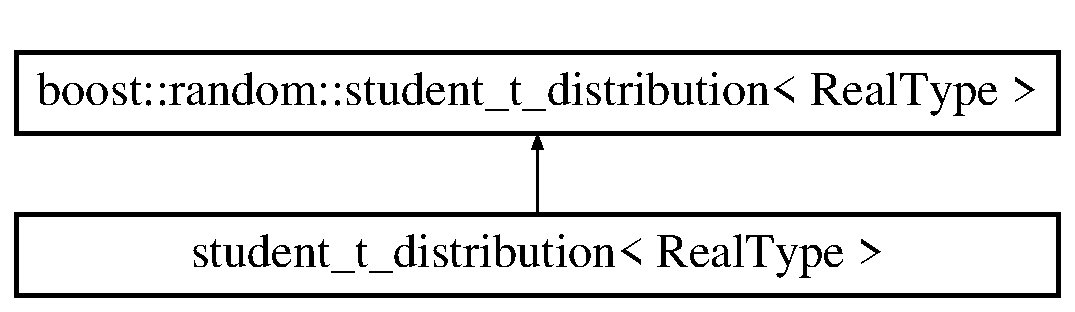
\includegraphics[height=2.000000cm]{structstudent__t__distribution}
\end{center}
\end{figure}
\subsection*{Public Member Functions}
\begin{DoxyCompactItemize}
\item 
\mbox{\Hypertarget{structstudent__t__distribution_a09042926811e047e71a2aefdfefc6ce3}\label{structstudent__t__distribution_a09042926811e047e71a2aefdfefc6ce3}} 
\mbox{\hyperlink{structstudent__t__distribution_a09042926811e047e71a2aefdfefc6ce3}{student\+\_\+t\+\_\+distribution}} (Real\+Type \mbox{\hyperlink{structstudent__t__distribution_af79519cdd38c501e1d67de31c93f3daf}{alpha}})
\begin{DoxyCompactList}\small\item\em construct an instnace give alpha \end{DoxyCompactList}\item 
\mbox{\Hypertarget{structstudent__t__distribution_a233da5eb814ed07f779a5005478df253}\label{structstudent__t__distribution_a233da5eb814ed07f779a5005478df253}} 
Real\+Type \mbox{\hyperlink{structstudent__t__distribution_a233da5eb814ed07f779a5005478df253}{cdf}} (Real\+Type x, bool lower\+\_\+tail=true) const
\begin{DoxyCompactList}\small\item\em return the cdf or the complement of the cdf \end{DoxyCompactList}\item 
\mbox{\Hypertarget{structstudent__t__distribution_a811239357f8d470db5c4c45bf0ddf996}\label{structstudent__t__distribution_a811239357f8d470db5c4c45bf0ddf996}} 
Real\+Type \mbox{\hyperlink{structstudent__t__distribution_a811239357f8d470db5c4c45bf0ddf996}{pdf}} (Real\+Type x) const
\begin{DoxyCompactList}\small\item\em return the probability density function at x \end{DoxyCompactList}\item 
\mbox{\Hypertarget{structstudent__t__distribution_abf87bfa9961e9ece0caa75fd545db2b2}\label{structstudent__t__distribution_abf87bfa9961e9ece0caa75fd545db2b2}} 
Real\+Type \mbox{\hyperlink{structstudent__t__distribution_abf87bfa9961e9ece0caa75fd545db2b2}{quantile}} (Real\+Type p) const
\begin{DoxyCompactList}\small\item\em return the quantile for probability p \end{DoxyCompactList}\item 
\mbox{\Hypertarget{structstudent__t__distribution_af79519cdd38c501e1d67de31c93f3daf}\label{structstudent__t__distribution_af79519cdd38c501e1d67de31c93f3daf}} 
Real\+Type \mbox{\hyperlink{structstudent__t__distribution_af79519cdd38c501e1d67de31c93f3daf}{alpha}} () const
\begin{DoxyCompactList}\small\item\em return the alpha = n of the distribution \end{DoxyCompactList}\item 
\mbox{\Hypertarget{structstudent__t__distribution_a5a81f4c1765c03864367ebd280c0a507}\label{structstudent__t__distribution_a5a81f4c1765c03864367ebd280c0a507}} 
Real\+Type \mbox{\hyperlink{structstudent__t__distribution_a5a81f4c1765c03864367ebd280c0a507}{alpha\+\_\+stable}} () const
\begin{DoxyCompactList}\small\item\em return the alpha of the asymptotic stable distribution \end{DoxyCompactList}\item 
\mbox{\Hypertarget{structstudent__t__distribution_a40784121ffcf86b36f4a107bc128302a}\label{structstudent__t__distribution_a40784121ffcf86b36f4a107bc128302a}} 
Real\+Type \mbox{\hyperlink{structstudent__t__distribution_a40784121ffcf86b36f4a107bc128302a}{mean}} () const
\begin{DoxyCompactList}\small\item\em Return mean of distribution. \end{DoxyCompactList}\item 
\mbox{\Hypertarget{structstudent__t__distribution_a037a9539d0054965130936c3da1a5a56}\label{structstudent__t__distribution_a037a9539d0054965130936c3da1a5a56}} 
Real\+Type \mbox{\hyperlink{structstudent__t__distribution_a037a9539d0054965130936c3da1a5a56}{mad}} () const
\begin{DoxyCompactList}\small\item\em Return mean average deviation of the distribution. \end{DoxyCompactList}\item 
\mbox{\Hypertarget{structstudent__t__distribution_aa877e48840101ffcebbe9f844502f99f}\label{structstudent__t__distribution_aa877e48840101ffcebbe9f844502f99f}} 
Real\+Type \mbox{\hyperlink{structstudent__t__distribution_aa877e48840101ffcebbe9f844502f99f}{mad2}} () const
\begin{DoxyCompactList}\small\item\em Return the mad of the square of the distribution. \end{DoxyCompactList}\item 
\mbox{\Hypertarget{structstudent__t__distribution_acd9350d5f25a95f8120333237f810f6b}\label{structstudent__t__distribution_acd9350d5f25a95f8120333237f810f6b}} 
Real\+Type \mbox{\hyperlink{structstudent__t__distribution_acd9350d5f25a95f8120333237f810f6b}{ci}} (Real\+Type level=Real\+Type(.\+05)) const
\begin{DoxyCompactList}\small\item\em Return the confidence interval of the distribution. \end{DoxyCompactList}\item 
\mbox{\Hypertarget{structstudent__t__distribution_a16dd6f257065331e72960fb23c9c208e}\label{structstudent__t__distribution_a16dd6f257065331e72960fb23c9c208e}} 
Real\+Type \mbox{\hyperlink{structstudent__t__distribution_a16dd6f257065331e72960fb23c9c208e}{characteristic\+\_\+function}} (Real\+Type omega) const
\begin{DoxyCompactList}\small\item\em return the characteristic function of the distribution at omega \end{DoxyCompactList}\item 
\mbox{\Hypertarget{structstudent__t__distribution_ab757b6e129b2babe78af3d9105c4eed8}\label{structstudent__t__distribution_ab757b6e129b2babe78af3d9105c4eed8}} 
Real\+Type \mbox{\hyperlink{structstudent__t__distribution_ab757b6e129b2babe78af3d9105c4eed8}{characteristic\+\_\+function\+\_\+prime}} (Real\+Type omega) const
\begin{DoxyCompactList}\small\item\em return the derivative of the characteristic function at omega \end{DoxyCompactList}\end{DoxyCompactItemize}
\subsection*{Friends}
\begin{DoxyCompactItemize}
\item 
\mbox{\Hypertarget{structstudent__t__distribution_aee4aaa9b82b8248166aced167a23798c}\label{structstudent__t__distribution_aee4aaa9b82b8248166aced167a23798c}} 
{\footnotesize template$<$class charT , class traits $>$ }\\std\+::basic\+\_\+ostream$<$ charT, traits $>$ \& \mbox{\hyperlink{structstudent__t__distribution_aee4aaa9b82b8248166aced167a23798c}{operator$<$$<$}} (std\+::basic\+\_\+ostream$<$ charT, traits $>$ \&os, const \mbox{\hyperlink{structstudent__t__distribution}{student\+\_\+t\+\_\+distribution}} \&dist)
\begin{DoxyCompactList}\small\item\em Write distribution to std\+::ostream. \end{DoxyCompactList}\end{DoxyCompactItemize}


\subsection{Detailed Description}
\subsubsection*{template$<$class Real\+Type = double$>$\newline
struct student\+\_\+t\+\_\+distribution$<$ Real\+Type $>$}

Instances of class \mbox{\hyperlink{structstudent__t__distribution}{student\+\_\+t\+\_\+distribution}} give random variates for a student t distribution with parameter n = alpha. 

The documentation for this struct was generated from the following file\+:\begin{DoxyCompactItemize}
\item 
/\+Users/jdunn/\+Documents/\+X\+Code/how\+\_\+much\+\_\+data/include/\mbox{\hyperlink{student__t__distribution_8h}{student\+\_\+t\+\_\+distribution.\+h}}\end{DoxyCompactItemize}

\chapter{File Documentation}
\hypertarget{exponential__distribution_8h}{}\section{/\+Users/jdunn/\+Documents/\+X\+Code/how\+\_\+much\+\_\+data/convolution\+\_\+test/exponential\+\_\+distribution.h File Reference}
\label{exponential__distribution_8h}\index{/\+Users/jdunn/\+Documents/\+X\+Code/how\+\_\+much\+\_\+data/convolution\+\_\+test/exponential\+\_\+distribution.\+h@{/\+Users/jdunn/\+Documents/\+X\+Code/how\+\_\+much\+\_\+data/convolution\+\_\+test/exponential\+\_\+distribution.\+h}}
{\ttfamily \#include $<$boost/random.\+hpp$>$}\newline
{\ttfamily \#include $<$boost/math/distributions/exponential.\+hpp$>$}\newline
\subsection*{Classes}
\begin{DoxyCompactItemize}
\item 
struct \mbox{\hyperlink{structexponential__distribution}{exponential\+\_\+distribution$<$ Real\+Type $>$}}
\begin{DoxyCompactList}\small\item\em instnaces of sturct \mbox{\hyperlink{structexponential__distribution}{exponential\+\_\+distribution}} generate random variates for exponential distribution \end{DoxyCompactList}\end{DoxyCompactItemize}

\hypertarget{lognormal__distribution_8h}{}\section{/\+Users/jdunn/\+Documents/\+X\+Code/how\+\_\+much\+\_\+data/convolution\+\_\+test/lognormal\+\_\+distribution.h File Reference}
\label{lognormal__distribution_8h}\index{/\+Users/jdunn/\+Documents/\+X\+Code/how\+\_\+much\+\_\+data/convolution\+\_\+test/lognormal\+\_\+distribution.\+h@{/\+Users/jdunn/\+Documents/\+X\+Code/how\+\_\+much\+\_\+data/convolution\+\_\+test/lognormal\+\_\+distribution.\+h}}
{\ttfamily \#include $<$iostream$>$}\newline
{\ttfamily \#include $<$iomanip$>$}\newline
{\ttfamily \#include $<$complex$>$}\newline
{\ttfamily \#include $<$string$>$}\newline
{\ttfamily \#include $<$memory$>$}\newline
{\ttfamily \#include $<$boost/random.\+hpp$>$}\newline
{\ttfamily \#include $<$boost/math/constants/constants.\+hpp$>$}\newline
{\ttfamily \#include $<$boost/math/distributions/lognormal.\+hpp$>$}\newline
{\ttfamily \#include $<$boost/math/special\+\_\+functions/erf.\+hpp$>$}\newline
{\ttfamily \#include $<$boost/math/quadrature/gauss\+\_\+kronrod.\+hpp$>$}\newline
{\ttfamily \#include $<$boost/math/quadrature/exp\+\_\+sinh.\+hpp$>$}\newline
{\ttfamily \#include \char`\"{}p\+\_\+spline.\+h\char`\"{}}\newline
\subsection*{Classes}
\begin{DoxyCompactItemize}
\item 
struct \mbox{\hyperlink{structlognormal__distribution}{lognormal\+\_\+distribution$<$ Real\+Type $>$}}
\begin{DoxyCompactList}\small\item\em a class with functions related to the lognormal distribution. \end{DoxyCompactList}\end{DoxyCompactItemize}

\hypertarget{pareto__distribution_8h}{}\section{/\+Users/jdunn/\+Documents/\+X\+Code/how\+\_\+much\+\_\+data/convolution\+\_\+test/pareto\+\_\+distribution.h File Reference}
\label{pareto__distribution_8h}\index{/\+Users/jdunn/\+Documents/\+X\+Code/how\+\_\+much\+\_\+data/convolution\+\_\+test/pareto\+\_\+distribution.\+h@{/\+Users/jdunn/\+Documents/\+X\+Code/how\+\_\+much\+\_\+data/convolution\+\_\+test/pareto\+\_\+distribution.\+h}}
{\ttfamily \#include $<$iostream$>$}\newline
{\ttfamily \#include $<$sstream$>$}\newline
{\ttfamily \#include $<$complex$>$}\newline
{\ttfamily \#include $<$random$>$}\newline
{\ttfamily \#include $<$boost/math/quadrature/gauss\+\_\+kronrod.\+hpp$>$}\newline
{\ttfamily \#include $<$boost/math/constants/constants.\+hpp$>$}\newline
{\ttfamily \#include $<$string$>$}\newline
\subsection*{Classes}
\begin{DoxyCompactItemize}
\item 
class \mbox{\hyperlink{classpareto__distribution}{pareto\+\_\+distribution$<$ Real\+Type $>$}}
\begin{DoxyCompactList}\small\item\em Instantiations of class template \mbox{\hyperlink{classpareto__distribution}{pareto\+\_\+distribution}} model a Pareto Type 2 distribution. \end{DoxyCompactList}\item 
class \mbox{\hyperlink{classpareto__distribution_1_1param__type}{pareto\+\_\+distribution$<$ Real\+Type $>$\+::param\+\_\+type}}
\end{DoxyCompactItemize}

\hypertarget{student__t__distribution_8h}{}\section{/\+Users/jdunn/\+Documents/\+X\+Code/how\+\_\+much\+\_\+data/convolution\+\_\+test/student\+\_\+t\+\_\+distribution.h File Reference}
\label{student__t__distribution_8h}\index{/\+Users/jdunn/\+Documents/\+X\+Code/how\+\_\+much\+\_\+data/convolution\+\_\+test/student\+\_\+t\+\_\+distribution.\+h@{/\+Users/jdunn/\+Documents/\+X\+Code/how\+\_\+much\+\_\+data/convolution\+\_\+test/student\+\_\+t\+\_\+distribution.\+h}}
{\ttfamily \#include $<$boost/random.\+hpp$>$}\newline
{\ttfamily \#include $<$boost/math/distributions/students\+\_\+t.\+hpp$>$}\newline
{\ttfamily \#include $<$boost/math/special\+\_\+functions/beta.\+hpp$>$}\newline
{\ttfamily \#include $<$boost/math/special\+\_\+functions/bessel.\+hpp$>$}\newline
\subsection*{Classes}
\begin{DoxyCompactItemize}
\item 
struct \mbox{\hyperlink{structstudent__t__distribution}{student\+\_\+t\+\_\+distribution$<$ Real\+Type $>$}}
\begin{DoxyCompactList}\small\item\em Instances of class \mbox{\hyperlink{structstudent__t__distribution}{student\+\_\+t\+\_\+distribution}} give random variates for a student t distribution with parameter n = alpha. \end{DoxyCompactList}\end{DoxyCompactItemize}

\hypertarget{monte__carlo__test_8cpp}{}\section{/\+Users/jdunn/\+Documents/\+X\+Code/how\+\_\+much\+\_\+data/monte\+\_\+carlo\+\_\+test/monte\+\_\+carlo\+\_\+test.cpp File Reference}
\label{monte__carlo__test_8cpp}\index{/\+Users/jdunn/\+Documents/\+X\+Code/how\+\_\+much\+\_\+data/monte\+\_\+carlo\+\_\+test/monte\+\_\+carlo\+\_\+test.\+cpp@{/\+Users/jdunn/\+Documents/\+X\+Code/how\+\_\+much\+\_\+data/monte\+\_\+carlo\+\_\+test/monte\+\_\+carlo\+\_\+test.\+cpp}}
{\ttfamily \#include $<$iostream$>$}\newline
{\ttfamily \#include $<$iomanip$>$}\newline
{\ttfamily \#include $<$string$>$}\newline
{\ttfamily \#include $<$sstream$>$}\newline
{\ttfamily \#include $<$fstream$>$}\newline
{\ttfamily \#include $<$random$>$}\newline
{\ttfamily \#include $<$vector$>$}\newline
{\ttfamily \#include $<$array$>$}\newline
{\ttfamily \#include $<$algorithm$>$}\newline
{\ttfamily \#include $<$numeric$>$}\newline
{\ttfamily \#include $<$mutex$>$}\newline
{\ttfamily \#include $<$thread$>$}\newline
{\ttfamily \#include $<$boost/timer/timer.\+hpp$>$}\newline
{\ttfamily \#include $<$boost/filesystem.\+hpp$>$}\newline
{\ttfamily \#include $<$boost/math/special\+\_\+functions/beta.\+hpp$>$}\newline
{\ttfamily \#include $<$boost/math/distributions/students\+\_\+t.\+hpp$>$}\newline
{\ttfamily \#include \char`\"{}pareto\+\_\+distribution.\+h\char`\"{}}\newline
{\ttfamily \#include \char`\"{}student\+\_\+t\+\_\+distribution.\+h\char`\"{}}\newline
{\ttfamily \#include \char`\"{}exponential\+\_\+distribution.\+h\char`\"{}}\newline
{\ttfamily \#include \char`\"{}lognormal\+\_\+distribution.\+h\char`\"{}}\newline
{\ttfamily \#include \char`\"{}taleb\+\_\+results.\+h\char`\"{}}\newline
\subsection*{Classes}
\begin{DoxyCompactItemize}
\item 
struct \mbox{\hyperlink{structKappaResult}{Kappa\+Result}}
\begin{DoxyCompactList}\small\item\em structure holding the results of a run for a single alpha \end{DoxyCompactList}\item 
struct \mbox{\hyperlink{structKappaResults}{Kappa\+Results}}
\begin{DoxyCompactList}\small\item\em structure holding the results of all runs \end{DoxyCompactList}\end{DoxyCompactItemize}
\subsection*{Functions}
\begin{DoxyCompactItemize}
\item 
{\footnotesize template$<$typename Real\+Type $>$ }\\Real\+Type \mbox{\hyperlink{monte__carlo__test_8cpp_a8bc12c575bef5adcd18ff54fed138db7}{rel\+\_\+err}} (Real\+Type a, Real\+Type b)
\begin{DoxyCompactList}\small\item\em return the relative error between two numbers \end{DoxyCompactList}\item 
{\footnotesize template$<$typename Real\+Type $>$ }\\vector$<$ Real\+Type $>$ \mbox{\hyperlink{monte__carlo__test_8cpp_a496196ea52c2a012c21f9dfbce88ff42}{quantile}} (const vector$<$ Real\+Type $>$ \&x, const vector$<$ Real\+Type $>$ \&probs)
\begin{DoxyCompactList}\small\item\em return quantiles of the ensemble of trials \end{DoxyCompactList}\item 
ostream \& \mbox{\hyperlink{monte__carlo__test_8cpp_abef86d57e5a2d6f59d7b6559f8ab0e25}{operator$<$$<$}} (ostream \&os, const \mbox{\hyperlink{structKappaResult}{Kappa\+Result}} \&k)
\begin{DoxyCompactList}\small\item\em output the results from a single run \end{DoxyCompactList}\item 
\mbox{\Hypertarget{monte__carlo__test_8cpp_a438174fcc3100be9441615ef06115383}\label{monte__carlo__test_8cpp_a438174fcc3100be9441615ef06115383}} 
ostream \& \mbox{\hyperlink{monte__carlo__test_8cpp_a438174fcc3100be9441615ef06115383}{operator$<$$<$}} (ostream \&os, \mbox{\hyperlink{structKappaResults}{Kappa\+Results}} \&ks)
\begin{DoxyCompactList}\small\item\em output the results for all runs \end{DoxyCompactList}\item 
{\footnotesize template$<$typename Dist $>$ }\\void \mbox{\hyperlink{monte__carlo__test_8cpp_a9c13d7165937292b4e6408264bd9bbe5}{calc\+\_\+kappa}} (unsigned int thread\+\_\+id, size\+\_\+t m, size\+\_\+t m\+\_\+ci\+\_\+limit, vector$<$ int $>$ ns, Dist dist, double ci\+\_\+level, \mbox{\hyperlink{structKappaResult}{Kappa\+Result}} $\ast$kp, bool verbose=false)
\begin{DoxyCompactList}\small\item\em the per thread cacluaiton engine \end{DoxyCompactList}\item 
{\footnotesize template$<$typename Dist $>$ }\\void \mbox{\hyperlink{monte__carlo__test_8cpp_a8154aa5a511b2a682f454661d9c507be}{calculate\+\_\+kappa}} (size\+\_\+t m, vector$<$ int $>$ ns, Dist dist, double ci\+\_\+level, \mbox{\hyperlink{structKappaResult}{Kappa\+Result}} $\ast$kp, bool verbose=false)
\begin{DoxyCompactList}\small\item\em calculate kappa for sums of iid variables at specified durations \end{DoxyCompactList}\item 
\mbox{\Hypertarget{monte__carlo__test_8cpp_a29d3334e2ee8e1ff561e3897ad2cc928}\label{monte__carlo__test_8cpp_a29d3334e2ee8e1ff561e3897ad2cc928}} 
void \mbox{\hyperlink{monte__carlo__test_8cpp_a29d3334e2ee8e1ff561e3897ad2cc928}{show\+\_\+usage}} (path p)
\begin{DoxyCompactList}\small\item\em show the usage. called when the wrong \# of arguments is used \end{DoxyCompactList}\item 
\mbox{\Hypertarget{monte__carlo__test_8cpp_ac0f2228420376f4db7e1274f2b41667c}\label{monte__carlo__test_8cpp_ac0f2228420376f4db7e1274f2b41667c}} 
int \mbox{\hyperlink{monte__carlo__test_8cpp_ac0f2228420376f4db7e1274f2b41667c}{main}} (int argc, const char $\ast$argv\mbox{[}$\,$\mbox{]})
\begin{DoxyCompactList}\small\item\em main program for convolution test with one input parameter the \# of trials \end{DoxyCompactList}\end{DoxyCompactItemize}
\subsection*{Variables}
\begin{DoxyCompactItemize}
\item 
\mbox{\Hypertarget{monte__carlo__test_8cpp_abc3d7525725b8e3ebc98d7a46cfd5e9e}\label{monte__carlo__test_8cpp_abc3d7525725b8e3ebc98d7a46cfd5e9e}} 
mutex \mbox{\hyperlink{monte__carlo__test_8cpp_abc3d7525725b8e3ebc98d7a46cfd5e9e}{kr\+\_\+mutex}}
\begin{DoxyCompactList}\small\item\em a mutex for writing to \mbox{\hyperlink{structKappaResults}{Kappa\+Results}} \end{DoxyCompactList}\item 
\mbox{\Hypertarget{monte__carlo__test_8cpp_aaf0af7d4d397479a7734afd9e67f7b98}\label{monte__carlo__test_8cpp_aaf0af7d4d397479a7734afd9e67f7b98}} 
mutex \mbox{\hyperlink{monte__carlo__test_8cpp_aaf0af7d4d397479a7734afd9e67f7b98}{cout\+\_\+mutex}}
\begin{DoxyCompactList}\small\item\em a mutex for writing to cout \end{DoxyCompactList}\end{DoxyCompactItemize}


\subsection{Function Documentation}
\mbox{\Hypertarget{monte__carlo__test_8cpp_a9c13d7165937292b4e6408264bd9bbe5}\label{monte__carlo__test_8cpp_a9c13d7165937292b4e6408264bd9bbe5}} 
\index{monte\+\_\+carlo\+\_\+test.\+cpp@{monte\+\_\+carlo\+\_\+test.\+cpp}!calc\+\_\+kappa@{calc\+\_\+kappa}}
\index{calc\+\_\+kappa@{calc\+\_\+kappa}!monte\+\_\+carlo\+\_\+test.\+cpp@{monte\+\_\+carlo\+\_\+test.\+cpp}}
\subsubsection{\texorpdfstring{calc\+\_\+kappa()}{calc\_kappa()}}
{\footnotesize\ttfamily template$<$typename Dist $>$ \\
void calc\+\_\+kappa (\begin{DoxyParamCaption}\item[{unsigned int}]{thread\+\_\+id,  }\item[{size\+\_\+t}]{m,  }\item[{size\+\_\+t}]{m\+\_\+ci\+\_\+limit,  }\item[{vector$<$ int $>$}]{ns,  }\item[{Dist}]{dist,  }\item[{double}]{ci\+\_\+level,  }\item[{\mbox{\hyperlink{structKappaResult}{Kappa\+Result}} $\ast$}]{kp,  }\item[{bool}]{verbose = {\ttfamily false} }\end{DoxyParamCaption})}



the per thread cacluaiton engine 


\begin{DoxyParams}[1]{Parameters}
\mbox{\tt in}  & {\em thread\+\_\+id} & the number of the thread used as seed for urng \\
\hline
\mbox{\tt in}  & {\em m} & the maximum \# of trials for mad \\
\hline
\mbox{\tt in}  & {\em m\+\_\+ci\+\_\+limit} & the maximum \# of trials for ci \\
\hline
\mbox{\tt in}  & {\em ns} & the durations to save \\
\hline
\mbox{\tt in}  & {\em dist} & the distribution \\
\hline
\mbox{\tt in}  & {\em ci\+\_\+level} & the confidence level for kappa\+\_\+ci \\
\hline
\mbox{\tt out}  & {\em kp} & the results \\
\hline
\mbox{\tt in}  & {\em verbose} & flag for trace infomation \\
\hline
\end{DoxyParams}
\mbox{\Hypertarget{monte__carlo__test_8cpp_a8154aa5a511b2a682f454661d9c507be}\label{monte__carlo__test_8cpp_a8154aa5a511b2a682f454661d9c507be}} 
\index{monte\+\_\+carlo\+\_\+test.\+cpp@{monte\+\_\+carlo\+\_\+test.\+cpp}!calculate\+\_\+kappa@{calculate\+\_\+kappa}}
\index{calculate\+\_\+kappa@{calculate\+\_\+kappa}!monte\+\_\+carlo\+\_\+test.\+cpp@{monte\+\_\+carlo\+\_\+test.\+cpp}}
\subsubsection{\texorpdfstring{calculate\+\_\+kappa()}{calculate\_kappa()}}
{\footnotesize\ttfamily template$<$typename Dist $>$ \\
void calculate\+\_\+kappa (\begin{DoxyParamCaption}\item[{size\+\_\+t}]{m,  }\item[{vector$<$ int $>$}]{ns,  }\item[{Dist}]{dist,  }\item[{double}]{ci\+\_\+level,  }\item[{\mbox{\hyperlink{structKappaResult}{Kappa\+Result}} $\ast$}]{kp,  }\item[{bool}]{verbose = {\ttfamily false} }\end{DoxyParamCaption})}



calculate kappa for sums of iid variables at specified durations 


\begin{DoxyParams}[1]{Parameters}
\mbox{\tt in}  & {\em m} & the number of scenarios \\
\hline
\mbox{\tt in}  & {\em ns} & the durations to save \\
\hline
\mbox{\tt in}  & {\em dist} & the distribution \\
\hline
\mbox{\tt in}  & {\em ci\+\_\+level} & the confidence level to use \\
\hline
\mbox{\tt out}  & {\em kp} & a ptr to the results \\
\hline
\mbox{\tt in}  & {\em verbose} & a flag to generate trace \\
\hline
\end{DoxyParams}
\mbox{\Hypertarget{monte__carlo__test_8cpp_abef86d57e5a2d6f59d7b6559f8ab0e25}\label{monte__carlo__test_8cpp_abef86d57e5a2d6f59d7b6559f8ab0e25}} 
\index{monte\+\_\+carlo\+\_\+test.\+cpp@{monte\+\_\+carlo\+\_\+test.\+cpp}!operator$<$$<$@{operator$<$$<$}}
\index{operator$<$$<$@{operator$<$$<$}!monte\+\_\+carlo\+\_\+test.\+cpp@{monte\+\_\+carlo\+\_\+test.\+cpp}}
\subsubsection{\texorpdfstring{operator$<$$<$()}{operator<<()}}
{\footnotesize\ttfamily ostream\& operator$<$$<$ (\begin{DoxyParamCaption}\item[{ostream \&}]{os,  }\item[{const \mbox{\hyperlink{structKappaResult}{Kappa\+Result}} \&}]{k }\end{DoxyParamCaption})}



output the results from a single run 


\begin{DoxyParams}[1]{Parameters}
\mbox{\tt in,out}  & {\em os} & the output stream \\
\hline
\mbox{\tt in}  & {\em k} & the sturct with results \\
\hline
\end{DoxyParams}
\mbox{\Hypertarget{monte__carlo__test_8cpp_a496196ea52c2a012c21f9dfbce88ff42}\label{monte__carlo__test_8cpp_a496196ea52c2a012c21f9dfbce88ff42}} 
\index{monte\+\_\+carlo\+\_\+test.\+cpp@{monte\+\_\+carlo\+\_\+test.\+cpp}!quantile@{quantile}}
\index{quantile@{quantile}!monte\+\_\+carlo\+\_\+test.\+cpp@{monte\+\_\+carlo\+\_\+test.\+cpp}}
\subsubsection{\texorpdfstring{quantile()}{quantile()}}
{\footnotesize\ttfamily template$<$typename Real\+Type $>$ \\
vector$<$Real\+Type$>$ quantile (\begin{DoxyParamCaption}\item[{const vector$<$ Real\+Type $>$ \&}]{x,  }\item[{const vector$<$ Real\+Type $>$ \&}]{probs }\end{DoxyParamCaption})}



return quantiles of the ensemble of trials 


\begin{DoxyParams}[1]{Parameters}
\mbox{\tt in}  & {\em x} & the result by trial \\
\hline
\mbox{\tt in}  & {\em probs} & the desired probabilities \\
\hline
\end{DoxyParams}
\mbox{\Hypertarget{monte__carlo__test_8cpp_a8bc12c575bef5adcd18ff54fed138db7}\label{monte__carlo__test_8cpp_a8bc12c575bef5adcd18ff54fed138db7}} 
\index{monte\+\_\+carlo\+\_\+test.\+cpp@{monte\+\_\+carlo\+\_\+test.\+cpp}!rel\+\_\+err@{rel\+\_\+err}}
\index{rel\+\_\+err@{rel\+\_\+err}!monte\+\_\+carlo\+\_\+test.\+cpp@{monte\+\_\+carlo\+\_\+test.\+cpp}}
\subsubsection{\texorpdfstring{rel\+\_\+err()}{rel\_err()}}
{\footnotesize\ttfamily template$<$typename Real\+Type $>$ \\
Real\+Type rel\+\_\+err (\begin{DoxyParamCaption}\item[{Real\+Type}]{a,  }\item[{Real\+Type}]{b }\end{DoxyParamCaption})}



return the relative error between two numbers 


\begin{DoxyParams}[1]{Parameters}
\mbox{\tt in}  & {\em a} & the first number \\
\hline
\mbox{\tt in}  & {\em b} & the second number \\
\hline
\end{DoxyParams}

\hypertarget{pinelis__taleb__test_8cpp}{}\section{/\+Users/jdunn/\+Documents/\+X\+Code/how\+\_\+much\+\_\+data/pinelis\+\_\+taleb\+\_\+test/pinelis\+\_\+taleb\+\_\+test.cpp File Reference}
\label{pinelis__taleb__test_8cpp}\index{/\+Users/jdunn/\+Documents/\+X\+Code/how\+\_\+much\+\_\+data/pinelis\+\_\+taleb\+\_\+test/pinelis\+\_\+taleb\+\_\+test.\+cpp@{/\+Users/jdunn/\+Documents/\+X\+Code/how\+\_\+much\+\_\+data/pinelis\+\_\+taleb\+\_\+test/pinelis\+\_\+taleb\+\_\+test.\+cpp}}
{\ttfamily \#include $<$iostream$>$}\newline
{\ttfamily \#include $<$iomanip$>$}\newline
{\ttfamily \#include $<$string$>$}\newline
{\ttfamily \#include $<$sstream$>$}\newline
{\ttfamily \#include $<$fstream$>$}\newline
{\ttfamily \#include $<$vector$>$}\newline
{\ttfamily \#include $<$array$>$}\newline
{\ttfamily \#include $<$algorithm$>$}\newline
{\ttfamily \#include $<$mutex$>$}\newline
{\ttfamily \#include $<$thread$>$}\newline
{\ttfamily \#include $<$complex$>$}\newline
{\ttfamily \#include $<$boost/timer/timer.\+hpp$>$}\newline
{\ttfamily \#include $<$boost/filesystem.\+hpp$>$}\newline
{\ttfamily \#include $<$boost/math/constants/constants.\+hpp$>$}\newline
{\ttfamily \#include \char`\"{}adaptive\+\_\+integration.\+h\char`\"{}}\newline
{\ttfamily \#include \char`\"{}pareto\+\_\+distribution.\+h\char`\"{}}\newline
{\ttfamily \#include \char`\"{}student\+\_\+t\+\_\+distribution.\+h\char`\"{}}\newline
{\ttfamily \#include \char`\"{}exponential\+\_\+distribution.\+h\char`\"{}}\newline
{\ttfamily \#include \char`\"{}lognormal\+\_\+distribution.\+h\char`\"{}}\newline
{\ttfamily \#include \char`\"{}taleb\+\_\+results.\+h\char`\"{}}\newline
\subsection*{Classes}
\begin{DoxyCompactItemize}
\item 
struct \mbox{\hyperlink{structNumpunct}{Numpunct}}
\begin{DoxyCompactList}\small\item\em sturcture passed by imbue to ostreams to use commas in numbers \end{DoxyCompactList}\item 
struct \mbox{\hyperlink{structKappaResult}{Kappa\+Result}}
\begin{DoxyCompactList}\small\item\em the struct holding the resutls of a single alpha \end{DoxyCompactList}\item 
struct \mbox{\hyperlink{structKappaResults}{Kappa\+Results}}
\begin{DoxyCompactList}\small\item\em sturcture holding the results from all runs \end{DoxyCompactList}\item 
class \mbox{\hyperlink{classPinelisTalebIntegrand}{Pinelis\+Taleb\+Integrand$<$ Dist $>$}}
\begin{DoxyCompactList}\small\item\em Functor used in the integratoin of the Pinelis Taleb result. \end{DoxyCompactList}\item 
class \mbox{\hyperlink{classPinelisTalebIntegrand_3_01pareto__distribution_3_4_01_4}{Pinelis\+Taleb\+Integrand$<$ pareto\+\_\+distribution$<$$>$ $>$}}
\begin{DoxyCompactList}\small\item\em Functor used in the integration of the Pinelis Taleb result for pareto dist. \end{DoxyCompactList}\item 
class \mbox{\hyperlink{classPinelisTalebIntegrand_3_01exponential__distribution_3_4_01_4}{Pinelis\+Taleb\+Integrand$<$ exponential\+\_\+distribution$<$$>$ $>$}}
\begin{DoxyCompactList}\small\item\em Functor used in the integration of the Pinelis Taleb result for exp. dist. \end{DoxyCompactList}\end{DoxyCompactItemize}
\subsection*{Typedefs}
\begin{DoxyCompactItemize}
\item 
\mbox{\Hypertarget{pinelis__taleb__test_8cpp_a51303eefcc6fc2ae099ec7d41bb63bc8}\label{pinelis__taleb__test_8cpp_a51303eefcc6fc2ae099ec7d41bb63bc8}} 
using {\bfseries dcomplex} = std\+::complex$<$ double $>$
\end{DoxyCompactItemize}
\subsection*{Functions}
\begin{DoxyCompactItemize}
\item 
\mbox{\Hypertarget{pinelis__taleb__test_8cpp_a55838e0258803b20fc5a23ff2e68076e}\label{pinelis__taleb__test_8cpp_a55838e0258803b20fc5a23ff2e68076e}} 
Kronrod$<$ double $>$ {\bfseries k\+\_\+big} (10)
\item 
\mbox{\Hypertarget{pinelis__taleb__test_8cpp_a8bc12c575bef5adcd18ff54fed138db7}\label{pinelis__taleb__test_8cpp_a8bc12c575bef5adcd18ff54fed138db7}} 
{\footnotesize template$<$typename Real\+Type $>$ }\\Real\+Type \mbox{\hyperlink{pinelis__taleb__test_8cpp_a8bc12c575bef5adcd18ff54fed138db7}{rel\+\_\+err}} (Real\+Type a, Real\+Type b)
\begin{DoxyCompactList}\small\item\em return the relative differnece between two numbers \end{DoxyCompactList}\item 
\mbox{\Hypertarget{pinelis__taleb__test_8cpp_abef86d57e5a2d6f59d7b6559f8ab0e25}\label{pinelis__taleb__test_8cpp_abef86d57e5a2d6f59d7b6559f8ab0e25}} 
ostream \& \mbox{\hyperlink{pinelis__taleb__test_8cpp_abef86d57e5a2d6f59d7b6559f8ab0e25}{operator$<$$<$}} (ostream \&os, const \mbox{\hyperlink{structKappaResult}{Kappa\+Result}} \&k)
\begin{DoxyCompactList}\small\item\em output the results to an ostream \end{DoxyCompactList}\item 
\mbox{\Hypertarget{pinelis__taleb__test_8cpp_a438174fcc3100be9441615ef06115383}\label{pinelis__taleb__test_8cpp_a438174fcc3100be9441615ef06115383}} 
ostream \& \mbox{\hyperlink{pinelis__taleb__test_8cpp_a438174fcc3100be9441615ef06115383}{operator$<$$<$}} (ostream \&os, \mbox{\hyperlink{structKappaResults}{Kappa\+Results}} \&ks)
\begin{DoxyCompactList}\small\item\em output the results of all runs to an ostream \end{DoxyCompactList}\item 
{\footnotesize template$<$typename Dist $>$ }\\void \mbox{\hyperlink{pinelis__taleb__test_8cpp_a2427a1d2bfb7cea92c6d7c088701834a}{calculate\+\_\+kappa}} (vector$<$ int $>$ ns, Dist dist, \mbox{\hyperlink{structKappaResult}{Kappa\+Result}} \&k, int verbose=0)
\begin{DoxyCompactList}\small\item\em set up ranges and step sizes for one alpham pass calculation of cf to threads and use fft to estimate distribution \end{DoxyCompactList}\item 
void \mbox{\hyperlink{pinelis__taleb__test_8cpp_a29d3334e2ee8e1ff561e3897ad2cc928}{show\+\_\+usage}} (path p)
\begin{DoxyCompactList}\small\item\em show proper usage after improper command line argument \end{DoxyCompactList}\item 
\mbox{\Hypertarget{pinelis__taleb__test_8cpp_ac0f2228420376f4db7e1274f2b41667c}\label{pinelis__taleb__test_8cpp_ac0f2228420376f4db7e1274f2b41667c}} 
int \mbox{\hyperlink{pinelis__taleb__test_8cpp_ac0f2228420376f4db7e1274f2b41667c}{main}} (int argc, const char $\ast$argv\mbox{[}$\,$\mbox{]})
\begin{DoxyCompactList}\small\item\em main program for convolution\+\_\+testl \end{DoxyCompactList}\end{DoxyCompactItemize}
\subsection*{Variables}
\begin{DoxyCompactItemize}
\item 
\mbox{\Hypertarget{pinelis__taleb__test_8cpp_aeb74e37f5d1626bb0e05e7391f4f8df7}\label{pinelis__taleb__test_8cpp_aeb74e37f5d1626bb0e05e7391f4f8df7}} 
int {\bfseries noext} = 0
\item 
\mbox{\Hypertarget{pinelis__taleb__test_8cpp_a76dc1eb59eb70d501eb5f96c86a84afb}\label{pinelis__taleb__test_8cpp_a76dc1eb59eb70d501eb5f96c86a84afb}} 
double {\bfseries epsabs\+\_\+double} = 0
\item 
\mbox{\Hypertarget{pinelis__taleb__test_8cpp_a8d84692761e7fbedd1e19de3daca1a10}\label{pinelis__taleb__test_8cpp_a8d84692761e7fbedd1e19de3daca1a10}} 
double {\bfseries epsrel\+\_\+double} = 64 $\ast$ std\+::numeric\+\_\+limits$<$double$>$\+::epsilon()
\item 
\mbox{\Hypertarget{pinelis__taleb__test_8cpp_a093d9695bc7f56e2e457d8ccf15652c1}\label{pinelis__taleb__test_8cpp_a093d9695bc7f56e2e457d8ccf15652c1}} 
int {\bfseries limit} = 2000
\item 
\mbox{\Hypertarget{pinelis__taleb__test_8cpp_afb7e4031902d3574edd39d620ec1bfbe}\label{pinelis__taleb__test_8cpp_afb7e4031902d3574edd39d620ec1bfbe}} 
int {\bfseries verbose\+\_\+integration} = 0
\end{DoxyCompactItemize}


\subsection{Function Documentation}
\mbox{\Hypertarget{pinelis__taleb__test_8cpp_a2427a1d2bfb7cea92c6d7c088701834a}\label{pinelis__taleb__test_8cpp_a2427a1d2bfb7cea92c6d7c088701834a}} 
\index{pinelis\+\_\+taleb\+\_\+test.\+cpp@{pinelis\+\_\+taleb\+\_\+test.\+cpp}!calculate\+\_\+kappa@{calculate\+\_\+kappa}}
\index{calculate\+\_\+kappa@{calculate\+\_\+kappa}!pinelis\+\_\+taleb\+\_\+test.\+cpp@{pinelis\+\_\+taleb\+\_\+test.\+cpp}}
\subsubsection{\texorpdfstring{calculate\+\_\+kappa()}{calculate\_kappa()}}
{\footnotesize\ttfamily template$<$typename Dist $>$ \\
void calculate\+\_\+kappa (\begin{DoxyParamCaption}\item[{vector$<$ int $>$}]{ns,  }\item[{Dist}]{dist,  }\item[{\mbox{\hyperlink{structKappaResult}{Kappa\+Result}} \&}]{k,  }\item[{int}]{verbose = {\ttfamily 0} }\end{DoxyParamCaption})}



set up ranges and step sizes for one alpham pass calculation of cf to threads and use fft to estimate distribution 


\begin{DoxyParams}[1]{Parameters}
\mbox{\tt in}  & {\em ns} & the durations to calculate \\
\hline
\mbox{\tt in}  & {\em dist} & the distribution \\
\hline
\mbox{\tt out}  & {\em k} & the results \\
\hline
\mbox{\tt in}  & {\em verbose} & flag for trace \\
\hline
\end{DoxyParams}
\mbox{\Hypertarget{pinelis__taleb__test_8cpp_a29d3334e2ee8e1ff561e3897ad2cc928}\label{pinelis__taleb__test_8cpp_a29d3334e2ee8e1ff561e3897ad2cc928}} 
\index{pinelis\+\_\+taleb\+\_\+test.\+cpp@{pinelis\+\_\+taleb\+\_\+test.\+cpp}!show\+\_\+usage@{show\+\_\+usage}}
\index{show\+\_\+usage@{show\+\_\+usage}!pinelis\+\_\+taleb\+\_\+test.\+cpp@{pinelis\+\_\+taleb\+\_\+test.\+cpp}}
\subsubsection{\texorpdfstring{show\+\_\+usage()}{show\_usage()}}
{\footnotesize\ttfamily void show\+\_\+usage (\begin{DoxyParamCaption}\item[{path}]{p }\end{DoxyParamCaption})}



show proper usage after improper command line argument 


\begin{DoxyParams}[1]{Parameters}
\mbox{\tt in}  & {\em p} & the path of the executable \\
\hline
\end{DoxyParams}

%--- End generated contents ---

% Index
\backmatter
\newpage
\phantomsection
\clearemptydoublepage
\addcontentsline{toc}{chapter}{Index}
\printindex

\end{document}
